\subsection{Introduction générale, définitions et notations }
\subsubsection{Mot, item lexical, terme}
\label{sec:mot}

Une définition communément admise considère qu'un mot est une suite de
caractères graphiques formant une unité sémantique et pouvant être
distinguée par un séparateur (généralement un blanc typographique ou
un signe de ponctuation\footnote{Nous nous restreignons volontairement
  ici aux langues indo-européennes écrites.}) \cite{Larousse2004}
\cite{Robert2000}.  Toutefois cette définition reste relativement
floue et souvent inadéquate aux problèmes qui nous sont posés.\footnote{
Elle ne tient pas compte, par exemple, des locutions
non-connexes (où un mot peut s'intercaler dans la locution) comme \lexItem{mettre les pieds dans le plat}.}

Dans ce document, nous utiliserons donc une définition plus "lexicale" et, préférerons en toute
rigueur, \emph{item lexical} plutôt que \emph{mot}. Nous définissons
un item lexical comme \sentence{une suite de caractères formant une
  unité sémantique et pouvant constituer une entrée de dictionnaire}.
Ainsi, \lexItem{voiture}, \lexItem{clair}, \lexItem{être} tout comme
\lexItem{pomme de terre}, \lexItem{moulin à vent}, des locutions
verbales comme \lexItem{tirer le diable par la queue}, des mots ayant
un sens différent au singulier et au pluriel comme \lexItem{orgue} et
\lexItem{orgues}\footnote{Un \lexItem{orgue} est un instrument de
  musique tandis que des \lexItem{orgues} (au féminin) sont \sentence{
    en géologie, des prismes d'une grande régularité formés lors du
    refroidissement d'une coulée de lave, basaltique le plus souvent,
    perpendiculaire à la surface.}  \cite{Larousse2004}} et même des
termes techniques comme \lexItem{pompe bivalve à échappement central}
sont des items lexicaux. Nous réserverons \emph{item lexical}, \emph{lemme} ou
\emph{terme} pour la forme canonique (cf. morphologie
\ref{sec:niveau-morphologique}) tandis que nous utiliserons plutôt
\emph{mot} pour les formes fléchies. Habituellement, \emph{terme} est,
comme son nom l'indique, plutôt utilisé dans un cadre terminologique;
toutefois nous le considérerons ici dans une acception plus
large comme désignant une entrée d'un lexique général.  Ainsi, nous
considérerons \emph{terme} et \emph{lemme} comme parfaitement synonymes
d'\emph{item lexical}. Nous insistons sur \emph{item lexical} pour
bien mettre l'accent sur l'idée que ce qui nous importe ici est que ce
soit une entrée de dictionnaire.

En ce qui concerne les notations, les items lexicaux sont notés en
petits caractères, en italique et entre apostrophes (\lexItem{vie}),
les mots en petits caractères et entre guillemets (\mot{vie}).

\subsubsection{Niveaux de traitement linguistique}
\label{sec:niveaux}

Compréhension et production de textes peuvent se décomposer en une
suite de traitements symétriques. La compréhension, comme le présente
la figure \ref{fig:sequence-traitement-taln}, est constituée d'un
\emph{traitement morphologique} qui consiste à identifier les items
lexicaux possibles à partir d'une forme fléchie donnée, puis d'un
\emph{traitement syntaxique} qui cherche à identifier les relations
qui existent entre les mots d'une phrase (sujets, verbes, compléments,
\ldots), d'un \emph{traitement sémantique} qui cherche à capturer le
"sens" des phrases et enfin d'un \emph{traitement pragmatique} qui
consiste à trouver la signification complète d'un texte liée en grande
partie à la présupposition. Une phase de production est décomposable
en une séquence inverse. Cette décomposition reste théorique et un
certain nombre de cas d'ambiguïtés nécessite des informations issues
du niveau suivant.

Il serait illusoire de penser que l'analyse d'un énoncé ne consiste qu'à \emph{filtrer} des informations en se limitant, pour chaque niveau, à faire un choix parmi les possibilités
proposées au niveau précédent. En
effet, la complexité de la langue tant au niveau de la construction
des mots, des phrases, des idées qu'au niveau de son évolution
(parfois par l'apparition de nouvelles tournures, plus couramment de
nouveaux termes souvent de façon éphémère) laisse difficile voire
impossible une couverture totale des possibilités de chaque niveau. Ce
modèle par couches permet éventuellement à un niveau supérieur de
compléter les informations d'un niveau inférieur. Ainsi, dans le cas
où le niveau morphologique ignorerait l'existence de \lexItem{orgues}
(au pluriel) le niveau sémantique pourra, s'il connaît cette forme, la
lui indiquer.

\begin{figure}%[H]
  \centering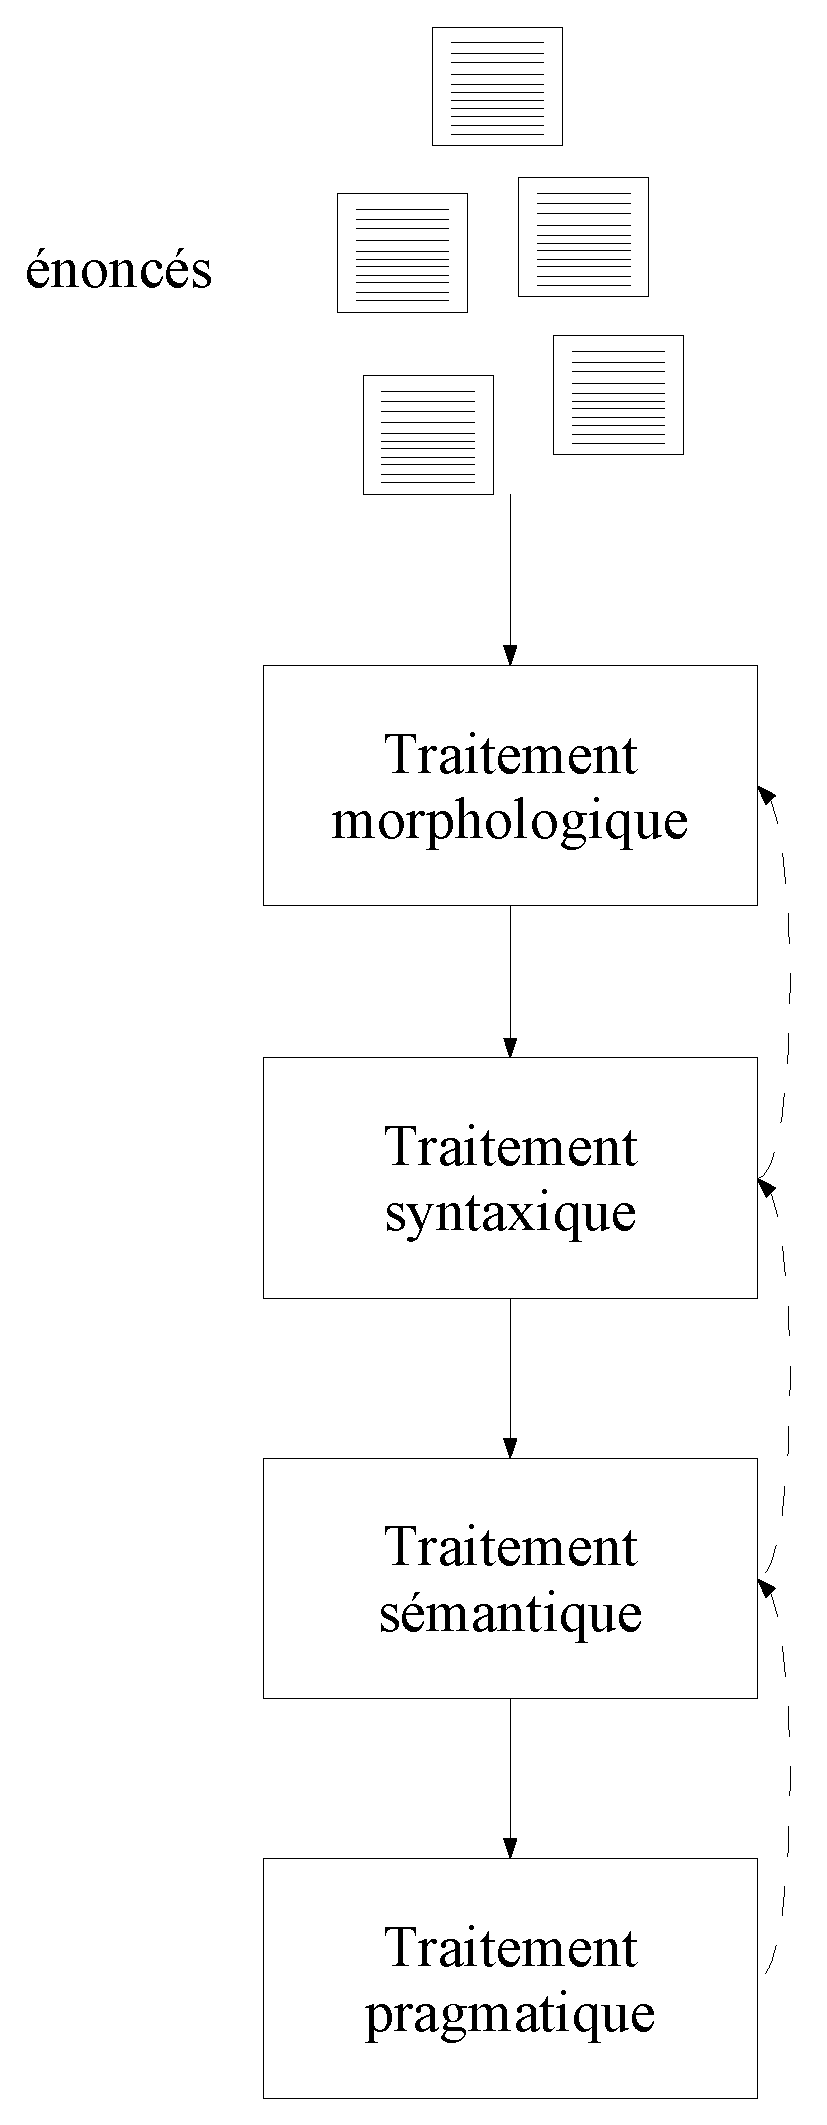
\includegraphics[height =
  12cm]{2_Etat-art/img/sequence-traitement-taln}

  \caption{Schéma général d'analyse de
    textes.}\label{fig:sequence-traitement-taln}
\end{figure}

Les traitements morphologiques et syntaxiques sont
relativement bien connus et étudiés en linguistique. Nous rappelons brièvement dans cette partie les principes sur lesquels ils reposent. Les deux niveaux suivants, en revanche, qui nous intéressent plus particulièrement dans le cadre de VidéoSense, sont encore très méconnus. Ils font l'objet de bien des théories et sont détaillés en \ref{sec:semantique}.

\subsubsection{Niveau morphologique}\label{sec:niveau-morphologique}

\paragraph{Niveau morphologique en linguistique}

En linguistique, la \emph{morphologie} est l'étude de la façon dont
sont formés les mots. On appelle \emph{morphèmes} les unités minimales
significatives qui constituent les mots. Par exemple, le mot
\mot{fleurs} est constitué de deux morphèmes : le radical (ou base)
correspondant à l'item \lexItem{fleur} et le suffixe marquant le
pluriel \emph{s}. Il existe deux catégories de morphèmes :

  \begin{itemize}
    
  \item les \emph{morphèmes lexicaux} qui correspondent aux items
    lexicaux ou à une légère variante;
  \item les \emph{morphèmes grammaticaux}, autrement appelés
    \emph{affixes}. Situé avant le radical, un affixe est dit
    \emph{préfixe}, après le radical, il est dit \emph{suffixe} et
    dans le radical, \emph{infixe}.

  \end{itemize}
  
  On peut distinguer deux types de formations morphologiques :

\begin{itemize}
\item \emph{flexion} : Les mots dits \emph{fléchis} comportent un
  radical et une ou plusieurs désinences. Les désinences sont les
  morphèmes porteurs des indications de nombre et de genre pour les
  noms, adjectifs et déterminants, de temps, de personnes et de mode
  pour les verbes. Ainsi, \mot{lisions} est constitué du radical
  \emph{lis-} issu de l'item \lexItem{lire}, de la désinence
  temporelle \emph{-i-} et de la désinence personnelle \emph{-ons}
  \citep{Lehmann1998}{132} tandis que \mot{rattes} est lui formé par
  \emph{rat} (radical) + \emph{te} (féminin) + s (pluriel). En aucun
  cas, la flexion ne modifie la catégorie syntaxique ;
  
\item \emph{dérivation} : On parle de dérivation lorsqu'un mot est
  formé à partir d'un autre en y adjoignant un ou plusieurs affixes
  porteurs de sens. Ainsi le sens du radical se trouve modifié et
  contrairement aux flexions, les dérivations peuvent amener à une
  nouvelle catégorie syntaxique. Si on prend pour exemple l'adjectif
  \mot{inacceptable}, il est formé de \emph{in} (affixe de contraire)
  + \emph{accept} (le radical, le verbe \lexItem{accepter}) +
  \emph{able} (affixe de possibilité).
\end{itemize}

Dans la suite, lorsque nous parlerons de la \emph{morphologie} pour un
item lexical ou un mot, il s'agira d'un abus de langage qui désigne
les informations que nous pouvons déduire de la morphologie de cet
item ou de ce mot. Ainsi, nous aurons les \emph{catégories
  grammaticales} (\emph{nom, pronom, adjectif, adverbe, etc.}), le
\emph{genre} (\emph{masculin, féminin, neutre}), le nombre
(\emph{singulier, pluriel}), le mode (\emph{transitif, intransitif}),
\ldots

La \emph{forme canonique} d'un mot est la forme de ce mot telle qu'on
peut la trouver comme entrée d'un dictionnaire par opposition à la
forme fléchie. Par définition, un item lexical est donc toujours dans
une forme canonique. Traditionnellement, suivant la nature de l'item,
une forme particulière est choisie :

\begin{itemize}
  
\item \emph{verbe} : à l'infinitif ;
\item \emph{nom} : au singulier (s'il existe) ;
\item \emph{adjectif} : au masculin singulier

\end{itemize}

On peut remarquer que, pour les mots invariables, formes fléchie et
canonique sont identiques.

\paragraph{Niveau morphologique en TALN\index{TALN}}

Habituellement, dans la phase d'analyse, il s'agit de
reconnaître les items lexicaux des textes. Il s'agira ainsi de
retrouver à partir d'un mot les possibilités de radical et d'affixe
ainsi que leurs caractéristiques grammaticales. Par exemple,
\lexItem{charges} peut être le nom féminin \lexItem{charge} au pluriel
comme le verbe \lexItem{charger} à l'indicatif ou au subjonctif
présent. Cette opération est aussi appelée \emph{lemmatisation}. Une
partie des ambiguïtés peut être levée au niveau syntaxique du
processus d'analyse.

\subsubsection{Niveau syntaxique}\label{sec:niveau-syntaxique}

\paragraph{Niveau syntaxique en linguistique}

La syntaxe étudie la manière dont les mots se combinent pour former
des phrases. % D'un point de vue purement grammatical, l'étude de la
%syntaxe concerne trois types d'objets :
%\begin{itemize}
%\item Le \emph{mot}, qui constitue la limite inférieure de l'étude
 % syntaxique et qui en est donc le constituant de base;
%\item La \emph{phrase}, qui constitue la limite supérieure de l'étude
 % syntaxique;
%\item Le \emph{syntagme} (ou \emph{groupe}), qui en est l'unité
 % intermédiaire.
%\end{itemize}
%Les mots et les syntagmes sont appelés \emph{constituants} de la
%phrase.  Des règles précises régissent les combinaisons entre les mots
%pour former des syntagmes et les combinaisons entre syntagmes pour
%former des phrases.  Ainsi, si le syntagme nominal \sentence{le chat}
%est correct, il n'en est pas de même pour \falsesentence{chat
  %le}\footnote{En linguistique, il est traditionnel de faire précéder
  %d'un astérisque une construction erronée en langue.} ni pour la
%phrase \falsesentence{Riche il et beau est.} dont l'expression
%conforme à la grammaire française serait plutôt \sentence{Il est beau
 % et riche.}.
%Si les mots ont des catégories grammaticales, les syntagmes ont aussi
%leurs propres catégories 
La \emph{structure syntaxique} des phrases, un arbre syntaxique résultant d'une analyse, peut être représentée au moyen de structures de {dépendances} ou de structures {syntagmatiques} (appelées également structures de \emph{constituants}). \\

Dans une représentation syntagmatique, les syntagmes (groupes de mot) ont, comme les mots, leurs propres catégories grammaticales (syntagme verbal, syntagme nominal, syntagme
prépositionnel, \ldots). Les règles syntaxiques permettent de décrire
chacun des constituants de la phrase :

\begin{itemize}
  
\item leur \emph{nature} : morphologie pour les mots, verbal, nominal,
  adjectival pour les syntagmes;
\item leur \emph{structure hiérarchique} : la manière dont les mots se
  regroupent pour former des syntagmes et la manière dont les
  syntagmes se regroupent pour former la phrase;
\item leur \emph{fonction syntaxique} : le rôle qu'ils tiennent à leur
  niveau de la hiérarchie : sujet, verbe, complément, \ldots
\end{itemize}

Dans une représentation en dépendances, la structure de la phrase est organisée autour d'un mot (par exemple le verbe) appelé la tête, auquel sont attachés des modificateurs (les noms sujets et compléments) ; chaque modificateur pouvant à son tour posséder des modificateurs. Le concept fondamental associé aux structures de dépendances est celui de \emph{relation} entre les mots. Etant donné deux mots du langage, on établit entre eux une relation de dominé (dépendant) à dominant (gouverneur) et on peut représenter cette relation par un arc entre deux n\oe uds, chaque n\oe ud étant étiqueté par un mot.

%Dans chaque syntagme, il y a un constituant qui a un rôle particulier,
%il a la fonction syntaxique de \emph{gouverneur}. Il s'agit du
%constituant principal du syntagme. Dans un syntagme nominal, il s'agit
%du nom, dans un syntagme verbal du verbe, dans une phrase, du syntagme
%sujet, etc.
%Habituellement, on présente l'analyse syntaxique d'une phrase sous la
%forme d'un \emph{arbre syntaxique}. Par exemple, l'arbre syntaxique de
%la phrase \sentence{Le petit chat boit du lait.} est présenté en
%figure \ref{fig:chatboit-lait-analyse-synt}.
%\begin{figure}%[H]
 % \centering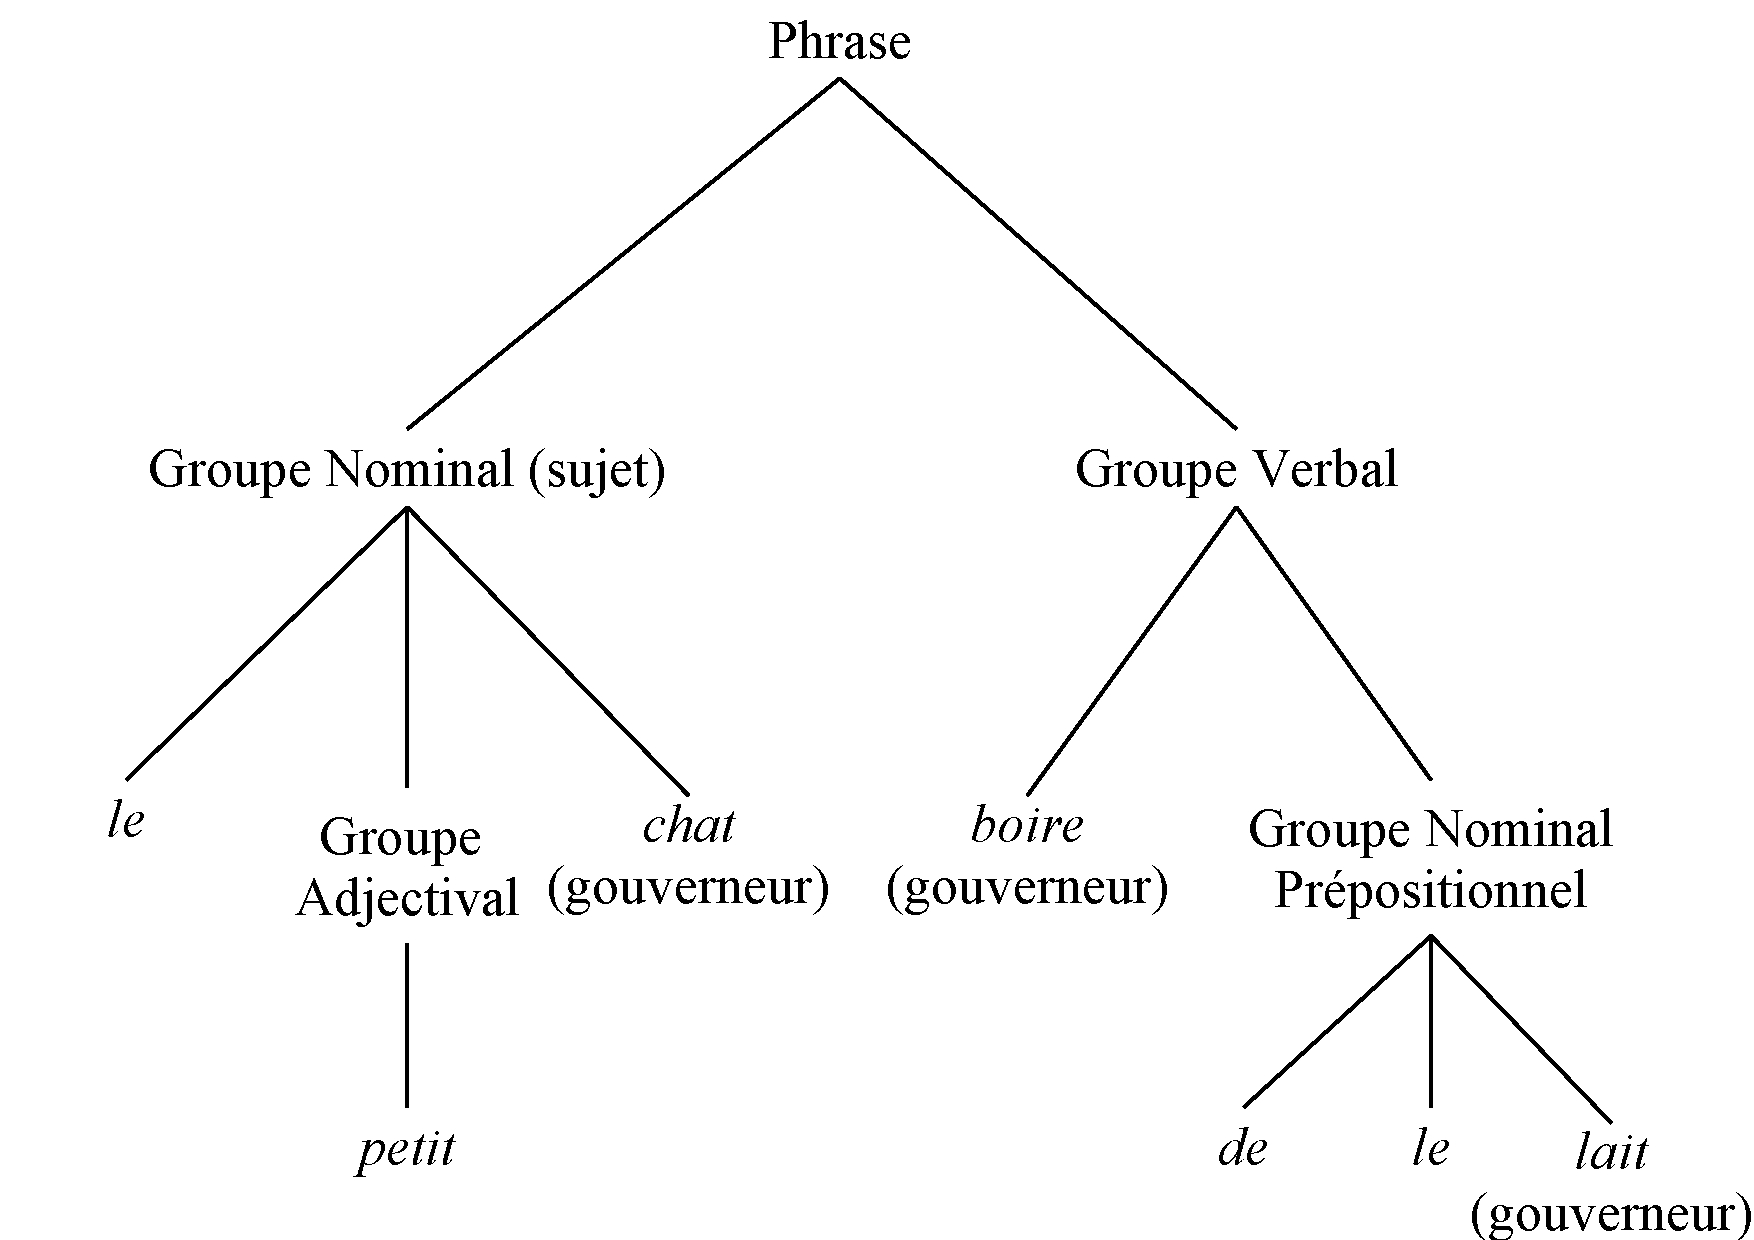
\includegraphics[width =
 % 12cm]{2_Etat-art/img/chatboit-lait-analyse-synt}

 % \caption{Arbre syntaxique syntagmatique de
  %  la phrase \sentence{Le petit chat boit du
     % lait.}.}\label{fig:chatboit-lait-analyse-synt}
%\end{figure}
\paragraph{Niveau syntaxique en
  TALN\index{TALN}}\label{sec:niveau-syntaxique-en-TALN}

Après la phase d'analyse morphologique, un certain nombre de solutions
sont envisageables pour les mots d'une phrase. Une analyse syntaxique
permet grâce aux règles de ne conserver que les solutions qui sont
possibles. Par exemple, prenons la phrase \sentence{Des charges
  supplémentaires seront retenues contre l'accusé.}. Le mot
\mot{charges}, comme nous l'avons vu dans la partie consacrée à la
morphologie, peut être le \emph{nom féminin} \lexItem{charge} au
pluriel comme le verbe \lexItem{charger} à l'indicatif ou au
subjonctif présent. La morphologie possible des mots constituant le
groupe nominal sujet \sentence{des charges supplémentaires} (pour
\mot{des}, \emph{déterminant pluriel}, pour \mot{supplémentaires},
\emph{adjectif masculin ou féminin pluriel}) rendent ici la seule
solution possible pour \mot{charges} \emph{nom féminin pluriel}.

%La recherche pour mettre au point des analyseurs fiables est encore florissante. 
La tâche pour mettre au point des analyseurs fiables est complexe puisqu'il n'existe pas à l'heure
actuelle de règles grammaticales pouvant couvrir l'ensemble des
phrases correctes dans aucune des langues existantes. Ainsi, deux
grandes familles d'analyseurs coexistent \citep{Bangalore1997}{5} :

\begin{itemize}
  
\item \emph{approche symbolique} : ces analyseurs se basent sur des
  règles grammaticales et nécessitent donc une recherche et une
  implémentation de ces règles. On peut citer dans cette catégorie,
  ARIANE \cite{Boitet2000}, l'analyseur du GREYC \cite{Vergne1998},
  IPF \cite{Wehrli1992}, SYGMART \cite{Chauche1984} ;
\item \emph{approche statistique} : ces analyseurs se basent sur des
  méthodes d'apprentissage à partir de corpus annotés manuellement ou
  automatiquement pour produire des règles pondérées \cite{Church1988,
    Collins1997, Munoz2000}.
\end{itemize}

Quelle que soit la technique utilisée, les analyseurs syntaxiques ne
renvoient pas tous un arbre syntaxique complet. %comme celui présenté en \ref{fig:chatboit-lait-analyse-synt}. 
%Ainsi, deux autres types de résultats sont possibles : renvoyer les relations entre les mots de la
%phrase ou produire une segmentation en syntagmes.

De même, une analyse syntaxique ne peut pas toujours lever toutes les
ambiguïtés.  Ainsi, certaines phrases comme \sentence{La petite brise
  la glace.} ne peuvent être totalement désambiguïsées à ce niveau de
traitement. Deux interprétations syntaxiques sont ici
possibles. Dans la première, \mot{petite} et \mot{glace} sont des
noms, \mot{brise} est la troisième personne du présent de l'indicatif
du verbe \lexItem{briser} (ie. une petite fille casse un miroir)
tandis que dans la deuxième, \mot{petite} correspond à l'adjectif
\lexItem{petit}, \mot{glace} au verbe \lexItem{glacer} et \mot{brise}
à l'item lexical \lexItem{brise} (ie. un léger vent donne froid à
quelqu'un ou quelque chose de féminin). Si syntaxiquement, il est
absolument impossible de lever l'ambiguïté, des informations de nature
sémantique et pragmatique sur cette phrase peuvent permettre d'émettre
des préférences.

%% viré d'ici SYGFRAN

\subsection[Qu'est-ce que le sens ? Comment le représenter ?]{Qu'est-ce que le sens ? Comment le représenter ?} \label{sec:semantique}
%\footnote{Partie fortement inspirée de \cite{schwab2005th}}

La sémantique est
l'étude du sens des énoncés. Bien que fort ancienne, puisque déjà étudiée par les philosophes de l'Antiquité, cette science fait encore
l'objet de bien des recherches notamment car
aucun moyen de décrire complètement le sens ne fait aujourd'hui
l'unanimité.

Peu d'ouvrages traitant de sémantique se risquent à donner ne serait ce qu'une esquisse de
définition du terme \lexItem{sens}. En effet, le sens est quelque
chose de difficile à décrire, souvent considéré dans
ces livres comme déjà acquis par le lecteur. \citep{Polguere2003}{98}
déroge à cette règle en reconnaissant explicitement le caractère
intuitif du sens et en présente une approche dont nous nous inspirons
largement ici. Alain Polguère propose comme définition du sens:

\vspace{0.3cm}

\begin{center}
  \textit{Le sens d'une expression linguistique est la propriété
    qu'elle partage\\ avec toutes ses paraphrases.}
\end{center}

Cette définition repose sur la notion d'équivalence entre
phrases, les paraphrases. Ces équivalences sont loin d'être rares en
langue, c'est même une des caractéristiques essentielles des langues
naturelles par rapport aux langages artificiels. Ainsi, pour Polguère,
la notion de paraphrase est reconnue comme un concept primitif possédé
par un locuteur qui permet de définir la notion de sens.

Le sens d'un énoncé est régi par le \emph{principe de
  compositionnalité sémantique} pour lequel\\ \sentence{le tout est
  calculable à partir du sens de ses parties}. Ainsi, un énoncé est
directement calculable (dans sa composition lexicale et sa structure
syntaxique) à partir de la combinaison du sens de chacun de ses
constituants \citep{Polguere2003}{134}. Par exemple, le sens d'une
phrase comme \sentence{L'enfant voit la mer.} est calculable à partir
:
\begin{itemize}
  
\item des items lexicaux \lexItem{le}, \lexItem{enfant},
  \lexItem{voir}, \lexItem{la}, \lexItem{mer};
  
\item des règles syntaxiques et morphologiques du français utilisées
  dans la phrase.

\end{itemize}

Il est souvent spécifié dans la littérature que les locutions
transgressent, au moins en partie, le principe de compositionnalité
sémantique. Dans notre approche où un mot est défini comme une des
formes fléchies d'un \emph{item lexical} (notion qui englobe les
locutions, cf.  \ref{sec:mot}), le problème ne se pose pas.

De nombreuses théories sur la sémantique ont été élaborées comme la
\emph{sémantique du prototype} \cite{Kleiber1990}, la \emph{sémantique
  distributionnelle} ou la \emph{sémantique structurale}. 
En traitement automatique du langage naturel, il s'agira de trouver le
sens d'un texte et pour cela, de désambiguïser le sens des mots qui le
composent. Prenons l'exemple de la phrase \sentence{La souris est
  reliée à l'ordinateur.}. Les traitements morphologique et syntaxique
permettront de savoir que le mot \mot{souris} correspond à l'item
\lexItem{souris}.  Considérons (pour simplifier) que ce terme a deux
sens : le premier correspondant à l'animal ; le deuxième à la souris
d'ordinateur. Le traitement sémantique permettra de trouver un
\emph{sens préférentiel} (dans notre exemple, la souris d'ordinateur).
Le traitement pragmatique, lui, choisira le "bon sens" en fonction du
contexte général. On peut imaginer que nous sommes dans un texte où
l'on parle d'une petite souris (l'animal) qui se promène et qui se
coince la queue dans le tiroir du lecteur de DVD; alors le sens
préférentiel du traitement sémantique ne sera pas celui choisi au
cours du traitement pragmatique.

Dans le cadre du projet VidéoSense, nous sommes confrontés aux trois questions principales
posées habituellement par ces problèmes :

\begin{itemize}
  
\item \emph{Comment représenter informatiquement le sens?}
  
\item \emph{Comment alors désambiguïser les mots d'un texte?}
  
\item \emph{Comment calculer le sens d'un texte?}

\end{itemize}

Plusieurs approches existent. Nous détaillons dans ce document principalement celles qui sont proches des méthodes employées en recherche d'information.

\subsection[Représentations d'origine distributionnaliste]{Représentations d'origine distributionnaliste\footnote{Partie fortement inspirée de \cite{schwab2005th}}}

\subsubsection{Approche distributionnelle}\label{sec:appr-distr}

La linguistique distributionnelle \cite{Harris1989} est le nom donné
aux recherches menées aux \'Etats-Unis par Zelig Sabbatai Harris
\epit{1909}{1992} à partir des années 1950 et qui poursuivaient celles
de Léonard Bloomfield \epit{1887}{1949}. L'analyse
distributionnelle cherche à décrire les objets linguistiques en
fonction du pouvoir d'associativité qu'ils possèdent ou ne possèdent
pas entre eux.  Ainsi, l'objectif premier de cette branche de la
linguistique est d'examiner les distributions des unités linguistiques
(phonèmes, morphèmes, mots) dans un corpus donné.

La linguistique distributionnelle considère que le sens d'un mot peut
être défini à partir de l'ensemble des contextes dans lequel il
apparaît, en d'autres termes, par l'ensemble des termes qui lui sont
cooccurrents dans un corpus. Par exemple, considérons ces quelques
phrases extraites du Web :

%\vspace{0,5cm}
\begin{center}
 \begin{itemize}
   
 \item \sentence{Seuls les chatons et pas les chats peuvent boire du
     lait de vache.}
   
 \item \sentence{Le pédiatre a diagnostiqué une allergie au lait de
     vache.}
   
 \item \sentence{Dis papa, c'est quoi cette bouteille de lait?}
   
 \item \sentence{À partir du lait, le fermier fait des fromages et des
     yaourts.}
  \end{itemize}
\end{center}
%\vspace{0,5cm}

Selon la linguistique distributionnelle, la sémantique de l'item
\lexItem{lait} peut ainsi être décrite grâce aux termes
\lexItem{vache}, \lexItem{bouteille}, \lexItem{fromage},
\lexItem{yaourt}, \lexItem{allergie}, \lexItem{chat},
\lexItem{chaton}, \ldots

On pourra dire que deux mots ont un sens proche s'ils sont employés
dans des contextes très voisins. Ce sont ces idées qui ont permis la
mise au point des vecteurs saltoniens et de leurs dérivés.

En informatique, le
sens d'un texte est donné par un vecteur dont les composantes
correspondent directement (modèle vectoriel standard) ou indirectement
(LSA) aux items lexicaux constituant le texte.

\subsubsection{Représentations saltoniennes} \label{sec:repr-salt}

À partir de la fin des années 1960, Gerard
Salton\footnote{\url{http://www.cs.cornell.edu/Info/Department/Annual95/Faculty/Salton.html}}\epit{1927}{1995}
professeur à la \emph{Cornell University}\footnote{Ithica, \'Etat de
  New York, \'Etats-Unis d'Amérique.}  met au point ce que l'on
appelle aujourd'hui le \emph{modèle vectoriel standard} (VSM pour
\emph{Vector Space Model}). Son application la plus connue est le
système de recherche documentaire SMART\footnote{Une version gratuite
  est accessible gratuitement pour la recherche à l'adresse
  \url{ftp://ftp.cs.cornell.edu/pub/smart/}} \cite{Smart1971,
  SalMac1983, Smart1991}. Suivant des idées issues de la linguistique
distributionnelle, les dimensions de l'espace vectoriel sont associées
à des \emph{termes d'indexation}, c'est-à-dire aux termes considérés
comme les plus discriminants dans le corpus de recherche.

\paragraph{Indexation des documents : fabrication des vecteurs}

Si t est le nombre de termes d'indexation, chaque document (et chaque
requête) est représenté par un vecteur à t dimensions tel que :
\begin{equation}
  \label{eq:vect-salton}
  D_i = (p_{i_1}, p_{i_2}, \ldots, p_{i_t})
\end{equation}
où $p_{i_k}$ est la k-ième composante de $D_i$ et a pour valeur le
poids du terme $T_k$ dans le document $D_i$. Le poids est souvent
calculé par une formule de type $\emph{tf}*\emph{idf}$ (\emph{term
  frequency $*$ inverse~document~frequency}). Les critères pris en compte sont :
\begin{itemize}
  
\item \emph{l'importance du terme dans le document} : on appelle
  fréquence d'un terme (\emph{term frequency}) le nombre de fois où ce
  terme apparaît, on parle aussi du \emph{nombre d'occurrences} ou de
  la \emph{fréquence d'occurrence}. Ce critère doit permettre de
  prendre en compte le fait que, plus le terme est présent, plus il a
  une importance dans le texte;
  
\item \emph{le pouvoir discriminant du terme} : les mots fréquents
  dans un texte ne sont pas forcément les plus discriminants par
  rapport au corpus entier. Par exemple, identifier un grand nombre
  d'occurrences du terme \lexItem{lait} dans un corpus dont le sujet
  central est justement le lait ne va pas permettre de différencier
  les divers documents. C'est pour contrebalancer ces cas que la prise
  en compte de la fréquence inverse en document est nécessaire. Il
  s'agit d'une évaluation de l'importance du terme dans l'ensemble du
  corpus. Plus le terme est présent, moindre sera l'idf.
\end{itemize}

Pour ces deux critères, plusieurs heuristiques peuvent être choisies.
Ces dernières sont généralement basées sur la fréquence du terme $t$
dans le document $d$, notée $f(t,d)$ ainsi que sur le nombre
d'occurrences du terme le plus fréquent de $d$ $\emph{Max}(f(t,d))$.
Par exemple, pour \emph{tf} on peut trouver :

\begin{itemize}
  
\item $\emph{tf} = f(t,d)$ si on considère que l'importance de l'item
  n'est donnée que par le nombre d'occurrences dans le texte ;
  
\item $\emph{tf} = log(f(t,d) + 1)$ : %la fonction logarithme augmente
  %fortement dans les petites valeurs (<100) et puis augmente de moins
  %en moins vite. 
  si on
  considère que l'on doit distinguer de façon moindre deux items ayant
  un nombre d'occurrences proches si leur fréquence dans le texte est
  importante et de façon plus importante dans le cas contraire ;
  
\item $\emph{tf} = \frac{f(t,d)}{Max(f(t,d))}$ si on considère que
  l'importance d'un terme est relative à celle du terme le plus
  présent dans le document. Notons que cette formule offre aussi
  l'avantage d'effectuer une certaine normalisation sur les vecteurs
  produits puisque le poids des composantes n'est pas influencé par la
  taille du document.

\end{itemize}

Pour \emph{idf}, les heuristiques sont moins nombreuses, on utilise en
général $log(\frac{N}{n})$ où $N$ est le nombre total de documents du
corpus et $n$ le nombre de documents du corpus où le terme apparaît au
moins une fois.

$\emph{tf}*\emph{idf}$ est donc la multiplication des valeurs de ces
deux critères. Ainsi on pourra choisir comme formule :

\begin{equation}
  \label{eq:tf-idf}
  \frac{f(t,d)}{Max(f(t,d))} \times log(\frac{N}{n})
\end{equation}

\paragraph{Exploitation des vecteurs}

La similarité entre deux documents $D_a$ et $D_b$ (ou entre un
document et une requête dans le cas de SMART) est donnée par la
formule (parfois dite \emph{du cosinus}) :

\begin{equation}
  \label{eq:salton-cos}
  \R^t\times\R^t \rightarrow [0,1] : \quad sim(D_a, D_b) =
\frac{\sum_{k=1}^{t}p_{a_k}\times
 p_{b_k}}{\sum_{k=1}^{t}p_a2 \times \sum_{k=1}^{t}p_b2}
\end{equation}

Les document les plus proches du document (ou de la requête) sont ceux
qui maximisent la similarité (l'angle entre les vecteurs est alors le
plus petit). On peut ainsi obtenir une liste ordonnée des documents
les plus proches d'un autre document ou, dans un cas de recherche
d'informations, de la requête.


\paragraph{Problèmes posés par la méthode}

Le premier problème du modèle vectoriel standard est aussi posé à
l'ensemble des représentations vectorielles : la mise à jour de la
base ne peut pas se faire de façon incrémentale. En effet,
l'utilisation de méthodes basées sur le critère \emph{idf} entraîne
obligatoirement le recalcul de l'ensemble des vecteurs lors de l'ajout
du moindre document au corpus.

Le second problème concerne le choix des termes d'indexation qui
entraîne trois conséquences notables :
\begin{itemize}
\item plus le nombre de termes retenus est important, plus fines sont
  les représentations;
\item plus le nombre de termes retenus est important, plus longues
  sont les opérations à réaliser (tant en indexation qu'en
  exploitation) et plus grande est la taille des données à stocker;
\item plus le nombre de termes retenus est important, moins la
  différence entre les documents les plus proches et les documents les
  plus éloignés d'un document donné est faible.
\end{itemize}

Suivant les corpus, le nombre d'item lexicaux différents peut être
relativement important. De la sorte, si la méthode utilisée pour
choisir les termes d'indexation ne fait que sélectionner ces items,
les vecteurs obtenus seront de très grande taille. L'approche doit
donc être menée d'une manière plus fine. Elle peut être basée sur un
antidictionnaire pour éliminer certains termes inadéquats, sur une
stemmatisation pour extraire la racine des termes (tous les mots ayant
la même racine seront alors considérés par la même composante), ou sur
une lemmatisation.


\subsubsection{Une approche psycholinguistique : LSA}

Le modèle LSA (\emph{Latent Semantic analysis}), appelé souvent aussi
LSI pour \emph{Latent Semantic indexing}, a été créé en
psycholinguistique pour simuler l'acquisition de connaissances d'un
être humain à partir de grands corpus de textes. Techniquement, LSA
est une variante du modèle vectoriel standard qui cherche à la fois à
réduire le nombre de dimensions des vecteurs et à améliorer la
représentation en rajoutant des informations sur la structure
sémantique implicite des unités linguistiques représentées par leurs
dépendances cachées \cite{DeeAll1990}.

En effet, les auteurs considèrent que le co-texte d'un item I
n'apporte pas suffisamment d'informations sur le sens puisqu'on ne
sait rien des liens sémantiques qu'entretiennent les mots de ce
co-texte avec les items qui n'apparaissent pas conjointement à I. Par
exemple, le co-texte de \lexItem{chaise} peut être donné par
\{\lexItem{s'asseoir}, \lexItem{repos}, \lexItem{bureau},
\lexItem{siège}, \lexItem{cuisine}, \ldots\} mais si un item comme
\lexItem{fauteuil} n'apparaît pas dans les co-textes de
\lexItem{chaise}, aucune information sur les rapports sémantiques
entre les deux termes ne sera disponible. L'idée est donc de croiser
les informations de cooccurrence de chaque item, c'est-à-dire ce que
l'on appelle les \emph{affinités de second ordre}
\cite{Grefenstette1994}. Dans LSA, le sens des termes est donc
engendré par les enchaînements de cooccurrences, à savoir les liens
implicites.  Pour résumer, dans LSA, deux items sont similaires si
leurs co-textes sont similaires. Deux co-textes sont similaires s'ils
comportent des termes similaires \cite{Lemaire2003}.

Dans un premier temps, la technique LSA consiste à construire à la
manière du modèle vectoriel standard des vecteurs correspondant aux
mots (dans ce cas l'unité du co-texte utilisée est généralement le
paragraphe) ou aux documents. Dans un deuxième temps, il s'agit de
regrouper les vecteurs dans une matrice et d'effectuer une
décomposition en valeurs propres.  Seuls les \emph{k} premiers
vecteurs propres sont pris en compte, l'espace de représentation est
donc réduit à $k$ dimensions. Une composante ne correspond pas à un
terme particulier, ce qui empêche toute interprétation directe et ne
rend possible que les comparaisons entre les vecteurs. La valeur de
$k$ ne doit pas être trop importante pour éviter le bruit et doit être
suffisamment faible pour éviter les trop grandes pertes d'information.
La valeur optimale de $k$ a été estimée empiriquement pour l'anglais
autour de 300 \cite{DeeAll1990}.

LSA utilise deux mesures. La première, identique à celle utilisée dans
le modèle vectoriel standard, permet d'estimer la similarité entre
deux mots ou deux groupes de mots, à partir du cosinus entre les
angles des vecteurs correspondants. La seconde mesure caractérise la
connaissance que LSA a sur un mot ou sur un groupe de mots, à partir
de la longueur du vecteur associé. Cette mesure, beaucoup moins
utilisée dans la littérature, dépend de la fréquence des mots et de la
diversité des contextes dans lesquels ils apparaissent.

Outre la recherche documentaire, la technique LSA a été utilisée dans
plusieurs applications comme l'extraction de métaphores
\cite{Kintsch2000} ou pour la segmentation automatique des textes
\cite{Bestgen2004}.

Dernièrement, \cite{GamalloOtero2010} montre que, comparativement à des modèles plus simples à mettre en œuvre,  LSA n'est efficace ni en temps de calcul ni en précision sur une tâche d'extraction de traductions.

\subsection{Représentations symboliques connexionnistes}

Ces représentations forment des graphes dont
les sommets correspondent à des objets lexicaux (item, acceptions) et
les arêtes à des relations sémantiques. Parmi ces relations, on peut distinguer les \emph{relations de
  hiérarchie} (\emph{hyperonymie}/\emph{hyponymie},
\emph{holonymie}/\emph{mérony\-mie}) des \emph{relations
  symétriques} (\emph{synonymie}/\emph{antonymie}). Les relations sémantiques sont décrites au moyen d'outils formels conçus sur le modèle des fonctions mathématiques : les fonctions lexicales \citep{Polguere2003}{131}, \citep{IntroLEC1995}{127}. Il existe autant de fonctions lexicales\index{fonctions lexicales}
qu'il existe de liens lexicaux et chaque fonction lexicale est
identifiée par un nom particulier.  Deux classes de fonctions
lexicales\index{fonctions lexicales} sont identifiées : les
\emph{fonctions lexicales paradigmatiques} et les \emph{fonctions
  lexicales syntagmatiques}.

%\subsubsection{Relations sémantiques et fonctions lexicales\index{fonctions
   % lexicales}} \label{sec:relat-semant-fct-lex}

%\paragraph{Relations sémantiques lexicales (ou relations
  %sémantiques externes)} \label{sec:rel-sem-externes}

%Nous avons déjà vu l'importance des paraphrases puisque ce sont elles
%qui nous ont permis de présenter ce que nous appelons le sens (cf.
%\ref{sec:semantique}). À travers ce petit dialogue, nous pouvons voir
%que communiquer c'est donc aussi pouvoir comprendre l'équivalence.
%Mais c'est également pouvoir comprendre les différences entre les
%phrases, savoir reformuler, développer, condenser ou améliorer son
%expression.  Il semblerait donc que les relations sémantiques
%lexicales soient nécessaires à la compréhension linguistique des
%individus. Elles nous permettent une certaine maîtrise du lexique.

%Les relations sémantiques structurent le lexique sur le plan
%paradigmatique\footnote{Le plan paradigmatique est le plan dans lequel
 % les termes sont unis par leur sens à l'intérieur du lexique.}. Nous
%présentons succinctement ici les six principales pour en donner une
%première idée nécessaire avant d'appréhender les fonctions
%lexicales\index{fonctions lexicales} et les réseaux sémantiques. Ces
%relations seront approfondies dans cette thèse lorsqu'il s'agira pour
%nous de les formaliser et de les modéliser à l'aide des vecteurs
%d'idées. Ces six relations sont de deux types, les \emph{relations de
 % hiérarchie} (\emph{hyperonymie}/\emph{hyponymie},
%\emph{holonymie}/\emph{mérony\-mie}) et les \emph{relations
  %symétriques} (\emph{synonymie}/\emph{antonymie}).

%\subparagraph{Relations de hiérarchie}

%Ces relations sont unidirectionnelles et transitives. Elles
%structurent ainsi le lexique de façon hiérarchique.  Il s'agit des
%deux paires hyponymie/hyperonymie et méronymie/holonymie. Si ${\cal
 % R}$ est une relation hiérarchique entre deux items $A$ et $B$, alors
%il existe une relation symétrique ${\cal \overline{R}}$ telle que :

%$${\cal R}(A, B) \equiv {\cal \overline{R}}(B, A)$$
%Il existe deux
%paires de relations hiérarchiques :
%\emph{hyponymie}/\emph{hyperonymie} et
%\emph{méronymie}/\emph{holonymie}.
% La relation d'hyponymie est la relation hiérarchique qui lie un hyponyme à un item plus général,
%l'hyperonyme. La relation d'hyperonymie est la relation inverse.
%Parmi les exemples d'hyponymie, on peut trouver :
%\lexItem{chat}$\backslash$\lexItem{animal},
%\lexItem{voilier}$\backslash$\lexItem{bateau},
%\lexItem{bateau}$\backslash$\lexItem{véhicule},
%\lexItem{rose}$\backslash$\lexItem{fleur}.


%\subparagraph{Relation tout-partie} La
%relation de méronymie est la relation hiérarchique qui lie la partie
%au tout. Un des éléments de la relation est une partie de l'autre
%élément. Les deux relations sont symétriques c'est-à-dire que le tout
%est l'holonyme de la partie tandis que la partie est le méronyme du
%tout. Parmi les exemples de méronymie, on peut trouver :
%\lexItem{voile}$\backslash$\lexItem{bateau} (\lexItem{voile} est
%méronyme de \lexItem{bateau}),
%\lexItem{page}$\backslash$\lexItem{livre},
%\lexItem{mur}$\backslash$\lexItem{maison},
%\lexItem{jour}$\backslash$\lexItem{mois}.


%\paragraph{Relations symétriques}

%Les relations symétriques sont la synonymie et l'antonymie. Comme leur
%nom l'indique, ces relations vérifient la propriété de symétrie.
%Ainsi, si ${\cal R}$ est une relation symétrique entre deux items $A$
%et $B$, alors :

%\begin{equation}
% \label{eq:symetrie}
 % {\cal R}(A, B) \equiv {\cal R}(B, A)
%\end{equation}

%En d'autres termes, si $A$ est synonyme (respectivement antonyme) de
%$B$, alors $B$ est synonyme (respectivement antonyme) de $A$.

%\subparagraph{Synonymie}

%La synonymie est la relation sémantique qu'il existe entre deux items
%lexicaux qui diffèrent par leur forme mais expriment le même sens ou
%un sens très proche.

%\lexItem{avion}$\backslash$\lexItem{aéroplane},
%\lexItem{écrivain}$\backslash$\lexItem{auteur},
%\lexItem{livre}$\backslash$\lexItem{bouquin},
%\lexItem{chat}$\backslash$\lexItem{matou}.

%\subparagraph{Antonymie}

%L'antonymie est la relation sémantique qui existe entre deux items
%lexicaux dont les sens s'opposent. Il existe trois types d'antonymie qui sont caractérisés par
%l'application ou non d'une propriété \cite{Schwab2001,Schwab2002a,Schwab2005}
%(\lexItem{vie}$\backslash$\lexItem{mort},
%\lexItem{certitude}$\backslash$\lexItem{incertitude}), une propriété
%étalonnable (\lexItem{riche}$\backslash$\lexItem{pauvre},
%\lexItem{chaud}$\backslash$\lexItem{froid}) ou un usage
%(\lexItem{père}$\backslash$\lexItem{fils},
%\lexItem{lune}$\backslash$\lexItem{soleil}).

%\paragraph{Fonctions lexicales de production\index{fonctions
   % lexicales! de production}}\label{sec:fonct-lexic-de-prod}

%Les fonctions lexicales\index{fonctions lexicales} ont été créées dans
%le cadre de la théorie linguistique \emph{sens-texte} (\emph{TST})
%élaborée par Igor Mel'\v{c}uk à Moscou avec des applications au russe
%jusqu'à la fin des années 1970 puis ensuite à Montréal pour le
%français.  L'un des outils mis au point est le \emph{Dictionnaire
 % explicatif et combinatoire du français contemporain} (\emph{DEC})
%dont l'objectif est de décrire, de façon systématique et rigoureuse,
%les informations permettant à un locuteur de construire toutes les
%expressions linguistiques correctes de n'importe quelle pensée et ce,
%dans n'importe quel contexte: c'est un dictionnaire de production.
%Cette lexicographie est très détaillée et très organisée, ce qui lui
%permet d'être exploitable pour la fois à un usage humain et pour un
%usage "machinal" en TALN\index{TALN}. Les items décrits dans le DEC le
%sont donc sous toutes leurs facettes: sémantique, syntaxique,
%lexico-combinatoire, morphologique, \ldots Le tableau de la figure
%\ref{fig:dico-autoriser} présente l'entrée résumée du DiCo pour un des
%sens de l'item \lexItem{autoriser} \cite{DICO1988}.
%\begin{figure}%[H]
  %\begin{center}
    %\begin{tabular}{|c|c|c|c|}
      %\hline
      %acception& \multicolumn{3}{c|}{autoriser.1}\\
      %\hline
      %propriétés grammaticales&\multicolumn{3}{c|}{\emph{verbe}}\\
      %\hline
      %formule sémantique&\multicolumn{3}{c|}{donner le droit de : X autorise Y à Z.}\\
      %\hline
      %&1=X&2=Y&3=Z\\
      %\cline{2-4}
      %régime 1&\multicolumn{1}{p{2cm}|}{1. N}&\multicolumn{1}{p{2cm}|}{2. N}&\multicolumn{1}{p{2cm}|}{3.  \emph{à} N}\\
     % &&\multicolumn{1}{r|}{\emph{obligatoire}}&\\
     %\cline{2-4}
     % &\multicolumn{3}{c|}{\sentence{Le docteur autorise l'avion à Pierre.}}\\
      %\hline
     % &1=X&2=Z&3=Y\\
      %\cline{2-4}
      %régime 2&\multicolumn{1}{p{2cm}|}{1. N}&\multicolumn{1}{p{2cm}|}{2. N}&\multicolumn{1}{p{2cm}|}{3.  \emph{à} V}\\

%&&\multicolumn{1}{r|}{\emph{obligatoire}}&\multicolumn{1}{r|}{\emph{obligatoire}}\\
    % \cline{2-4}
      %&\multicolumn{3}{c|}{\sentence{Le docteur autorise Pierre à embarquer.}}\\
      %\hline
      %&\multicolumn{1}{l}{$Syn_\cap$} & \multicolumn{2}{l|}{ permettre.I laisser.2, tolérer}\\
      %&\multicolumn{1}{l}{$Anti$} & \multicolumn{2}{l|}{interdire I, ne pas autoriser I.1}\\
      %Fonctions lexicales&\multicolumn{1}{l}{$Anti_\subset$} & \multicolumn{2}{l|}{proscrire}\\
      %&\multicolumn{1}{l}{$Anti_\cap$} & \multicolumn{2}{l|}{défendre, s'opposer, empêcher,\ldots}\\
      %&\multicolumn{1}{l}{$S_0$} & \multicolumn{2}{l|}{autorisation}\\
      %&\multicolumn{1}{l}{$Magn$} & \multicolumn{2}{l|}{formellement, expressément}\\
      %\hline
    %\end{tabular}
    %\caption{Entrée résumée du DiCo pour l'item
      %\lexItem{autoriser} \cite{DICO1988}} \label{fig:dico-autoriser}
  %\end{center}
%\end{figure} 

%Les fonctions lexicales\index{fonctions lexicales} ont été définies
%dans le cadre de la TST pour décrire les relations sémantiques
%lexicales au moyen d'un outil formel conçu sur le modèle des fonctions
%mathématiques \citep{Polguere2003}{131}, \citep{IntroLEC1995}{127}.

%Une fonction lexicale $f$ décrit une relation existant entre un item
%lexical $I$ (l'\emph{argument} de $f$) et un ensemble d'items lexicaux
%$\{I_1, I_2,\ldots, I_n\}$ appelé la \emph{valeur} de l'application de
%$f$ à l'item $I$. La fonction lexicale $f$ est telle que :

%\begin{enumerate}
  
%\item l'expression $f(I)$ représente l'application de $f$ à l'item $I$
  %: $f(I)=\{I_1, I_2,\ldots, I_n\}$
  
%\item chaque élément de la valeur de $f(I)$ est lié à $I$ de la même
 % façon et remplit (à peu près) le même rôle : $\frac{f(I_1)}{I_1}
  %\approx \frac{f(I_2)}{I_2}$

%\end{enumerate}

%Ainsi, pour illustrer, la fonction lexicale de synonymie $Syn$
%modélise le rapport qu'entretiennent entre eux les termes
%\lexItem{livre} et \lexItem{bouquin} d'une part et \lexItem{chat} et
%\lexItem{matou} d'autre part. Mel'\v{c}uk note :

%$$\frac{\mbox{\lexItem{livre}}}{\mbox{\lexItem{bouquin}}} \approx
%\frac{\mbox{\lexItem{chat}}}{\mbox{\lexItem{matou}}} \approx
%\frac{\mbox{\lexItem{matou}}}{\mbox{\lexItem{chat}}}$$

%De même, la fonction lexicale d'antonymie $Anti$ modélise le rapport
%qu'entretiennent entre eux les termes \lexItem{certitude} et
%\lexItem{incertitude} d'une part et \lexItem{vie} et \lexItem{mort}
%d'autre part.

%$$\frac{\mbox{\lexItem{certitude}}}{\mbox{\lexItem{incertitude}}}
%\approx \frac{\mbox{\lexItem{vie}}}{\mbox{\lexItem{mort}}} \approx
%\frac{\mbox{\lexItem{mort}}}{\mbox{\lexItem{vie}}}$$

%Il existe autant de fonctions lexicales\index{fonctions lexicales}
%qu'il existe de liens lexicaux et chaque fonction lexicale est
%identifiée par un nom particulier.  Deux classes de fonctions
%lexicales\index{fonctions lexicales} sont identifiées : les
%\emph{fonctions lexicales paradigmatiques} et les \emph{fonctions
 % lexicales syntagmatiques}.

%\subparagraph{Fonctions lexicales paradigmatiques}

%Comme leur nom l'indique, les fonctions lexicales paradigmatiques
%formalisent les relations sémantiques. On distingue par exemple :

%\begin{itemize}
  
%\item \emph{Synonymie} ($Syn$) : \\$Syn($\lexItem{avion}$) = $
  %\lexItem{aéronef}, \lexItem{aéroplane}, \lexItem{coucou},\ldots
  
%\item \emph{Antonymie} ($Anti$) : \\ $Anti($certitude$) =
 % $\lexItem{incertitude}, \lexItem{doute}, \lexItem{scepticisme},
  %\ldots
  
%\item \emph{Générique} ($Gener$) : Les génériques sont les équivalents
 % des hyperonymes. \\$Gener($\lexItem{rose}$) = $ \lexItem{fleur};
 % $Gener($\lexItem{chat}$) = $\lexItem{animal}, \ldots
  
%\item \emph{Dérivés syntaxiques} : Ces fonctions associent à un item
  %sa contrepartie nominale (Substantification $S_0$), verbale
  %(verbalisation $V_0$), adjectivale (adjectivisation $A_0$) ou
  %adverbiale ($Adv_0$) :
  
  %$S_0$ (\lexItem{tuer}) = \lexItem{meurtre}, $S_0$ (\lexItem{vivre})
  %= \lexItem{vie}, $V_0$(\lexItem{serment}) = \lexItem{jurer},
  %$S_0$(\lexItem{jurer})=\lexItem{serment}
%\end{itemize}

%Les fonctions lexicales\index{fonctions lexicales} peuvent être
%indicées par des opérateurs ensemblistes pour indiquer des nuances de
%sens. Ainsi, on trouvera :

%\begin{itemize}
  
%\item $\subset$ pour indiquer une inclusion du sens de l'argument dans
  %la valeur de la fonction. On trouve ce cas avec les rapports
  %d'hyperonymie : $Syn_\subset($\lexItem{pigeon}$)=$\lexItem{oiseau} ;
  
%\item $\supset$ pour indiquer une inclusion du sens de la valeur dans
 % l'argument de la fonction :
  %$Syn_\supset($\lexItem{oiseau}$)=$\lexItem{pigeon} ;

  
%\item $\cap$ pour indiquer une intersection de sens. Ainsi
 % $Syn_\cap($\lexItem{jouer}$)=$\lexItem{s'amuser} puisqu'on peut
  %jouer sans s'amuser et s'amuser sans jouer.

%\end{itemize}

%\subparagraph{Fonctions lexicales syntagmatiques : collocations}
%\label{sec:fct-lex-syntagm}

%Dans toutes les langues, certaines combinaisons d'items lexicaux
%prévalent sur d'autres sans qu'il ne semble n'y avoir de motif logique. Par exemple, on parle de \sentence{dormir profondément}
%plutôt que de \falsesentence{dormir intensément} ou
%\falsesentence{dormir totalement} pourtant aucune raison (du moins en
%synchronie) ne semble expliquer cette préférence. On parle, dans ces
%cas, de phénomène de \emph{collocation}.

%L'énoncé $AB$ (ou $BA$) formé des items lexicaux $A$ et $B$ est une
%collocation si, pour produire cette expression, le locuteur
%sélectionne $A$ librement d'après son sens alors qu'il sélectionne $B$
%pour exprimer un autre sens en fonction de $A$
%\citep{Polguere2003}{134}. On appelle $A$ \emph{base de la
  %collocation} et $B$ \emph{collocatif}. On peut citer comme exemples
%de collocations en français : \lexItem{tir}${}_{[=A]}$
%\lexItem{nourri}${}_{[=B]}$, \lexItem{peur}${}_{[=A]}$
%\lexItem{bleue}${}_{[=B]}$, \lexItem{forte}${}_{[=B]}$
%\lexItem{fièvre}${}_{[=A]}$,\lexItem{dormir}${}_{[=A]}$
%\lexItem{profondément}${}_{[=B]}$.

%Les fonctions lexicales paradigmatiques ont été créées pour rendre
%compte des collocations non seulement dans le rôle syntaxique que joue
%le collocatif auprès de la base mais aussi par le sens qu'il exprime.
%Parmi les fonctions lexicales syntagmatiques, on peut citer :

%\begin{itemize}
  
%\item $Bon$ qui marque une évaluation positive :
 % $Bon($\lexItem{choix}$)$ = \lexItem{bon} ;
  
%\item $Magn$ qui marque l'intensification :
 % $Magn($\lexItem{majorité}$) = $\lexItem{forte}, \lexItem{écrasante}.

%\end{itemize}

%ou leurs opposés :

%\begin{itemize}
  
%\item $AntiBon$ qui marque une évaluation négative :
  %$AntiBon($\lexItem{choix}$)$ = \lexItem{mauvais} ;
  
%\item $AntiMagn$ qui marque une modification inverse à
  %l'intensification : $AntiMagn($\lexItem{majorité}$) =
  %$\lexItem{cour\-te}, \lexItem{faible}.

%\end{itemize}

\subsubsection{Réseaux sémantiques}\label{sec:reseaux-semantiques}

Les réseaux sémantiques tirent leur origine de la psychologie
expérimentale et plus particulièrement des travaux concernant
l'organisation mentale des concepts, menés à la fin des années 1960  \cite{Quillian1968}.

%\paragraph{Origines}

%À la fin des années 1960, Alan Collins et Ross Quillian observent que,
%pour un être humain, le temps d'estimation de la validité d'une phrase
%comme \sentence{un chien est un mammifère} est plus long que celui
%d'une phrase comme \sentence{un chien est un animal}
%\cite{CollinsQuillian1969} \cite{CollinsQuillian1970}. Cette
%différence dans le délai de réaction semble liée au nombre d'individus
%de la classe \cite{JuolaAtkinson1971} \cite{LandauerFreedman1968}
%comme le montre l'expérience présentée dans la figure
%\ref{fig:temps_reaction}.

%\begin{figure}[h]%[H]
  %\centering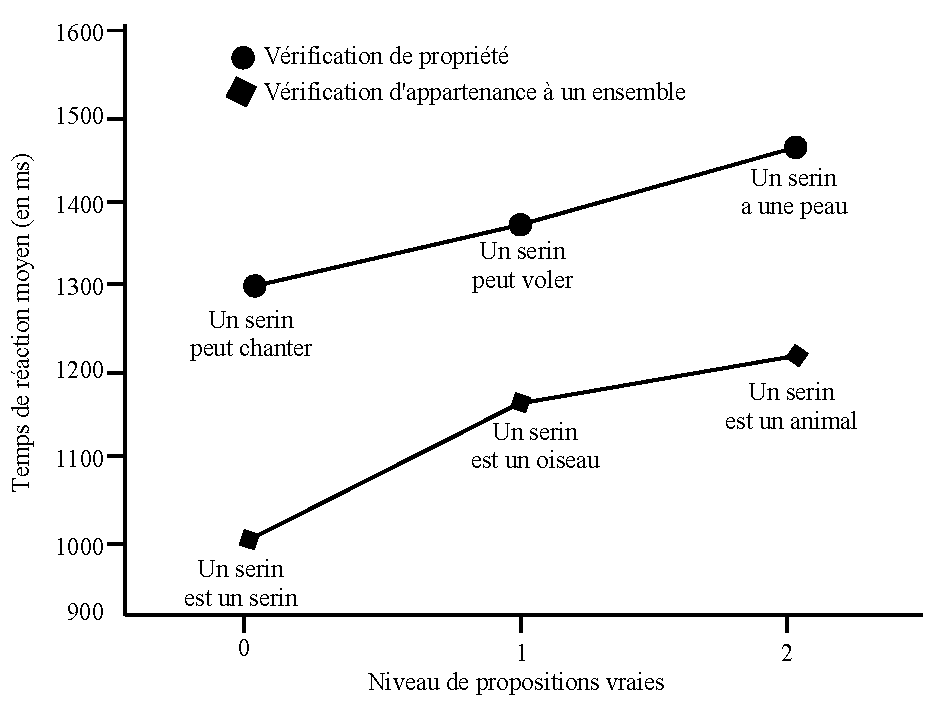
\includegraphics[width=10cm]{2_Etat-art/img/temps_reaction}

 %\caption{\small Vérification d'énoncés sémantiques : résultats
  % expérimentaux \cite{CollinsQuillian1969}}\label{fig:temps_reaction}
%\end{figure}

%Ces expériences semblent montrer que les informations associées à
%certains concepts sont transmissibles aux concepts hyponymes et ne
%sont pas mémorisées directement avec ceux-ci.  En d'autres termes, les
%concepts spécialisés héritent des propriétés et des attributs des
%concepts plus généraux auxquels ils sont associés et y adjoignent
%leurs propres propriétés et attributs. Ainsi, il s'agit d'un
%\emph{principe d'économie} reposant sur la mise en facteur des
%connaissances communes à plusieurs sortes d'objets \cite{Bernard2000}
%\cite{Sabah1988}. Par exemple, \lexItem{mammifère} met en facteur les
%propriétés et les attributs communs aux différentes espèces qui le
%composent (\lexItem{Homme}, \lexItem{chien}, \lexItem{lapin},\ldots)
%et qui en retour en héritent. Le figure \ref{fig:automate_Quillian}
%présente l'automate de Quillian qui est un exemple de hiérarchie
%centrée autour d'\lexItem{animal}.

%\begin{figure}[h]%[H]
  %\centering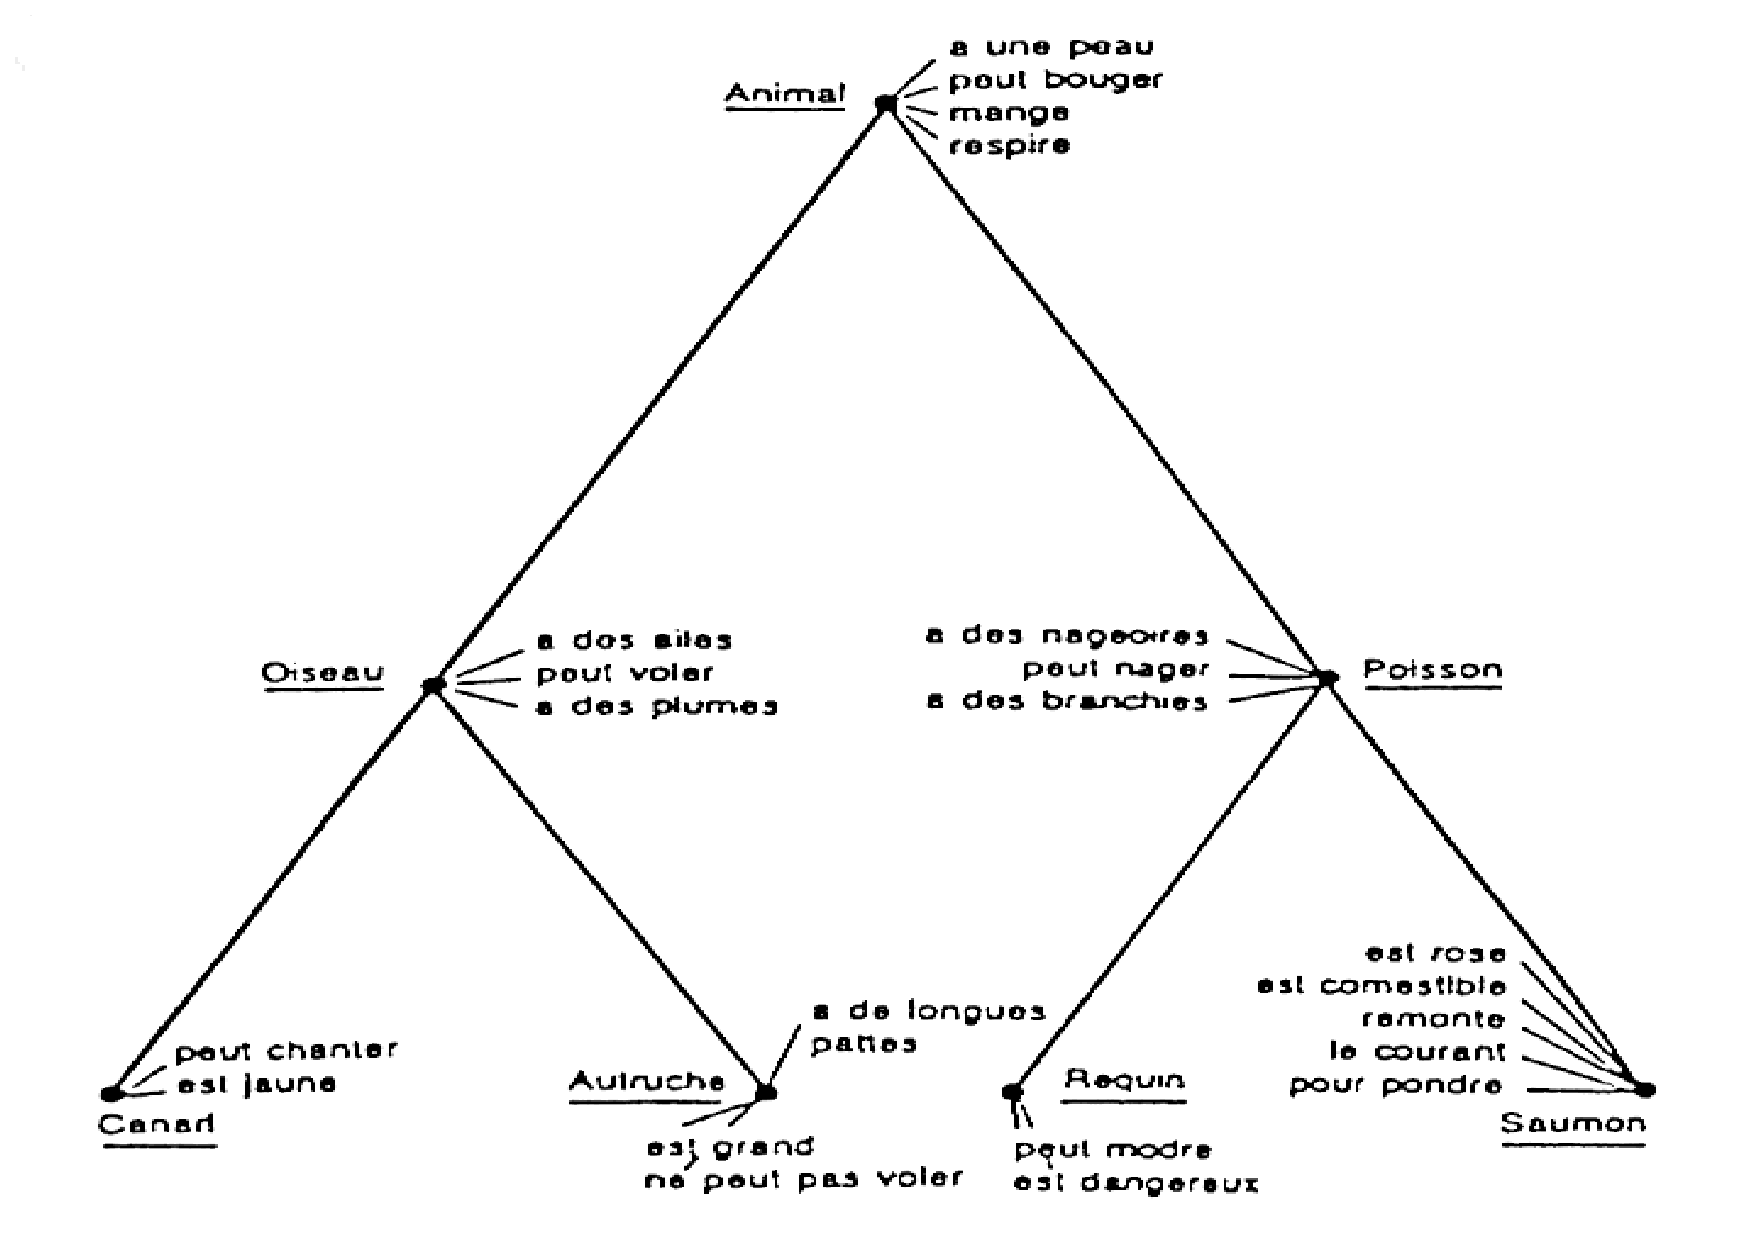
\includegraphics[height=10cm]{2_Etat-art/img/automate_Quillian}

 %\caption{L'automate de Quillian : hiérarchie centrée autour
  % d'\lexItem{animal}.}\label{fig:automate_Quillian}
%\end{figure}

%Plusieurs expériences dont celle d'Harold Goodglass \epit{1920}{2002}
%et Errol Baker concernant l'aphasie\footnote{L'aphasie est une perte
  %totale ou partielle du langage consécutive à une atteinte cérébrale.
  %Les personnes aphasiques ne peuvent plus (ou avec difficulté)
  %parler, comprendre, lire et écrire.
  %\url{http://membres.lycos.fr/aphasie/}} corroborent cette thèse
%\cite{GoodglassBaker1976}. Pour les sujets de l'expérience, il s'agit
%d'associer ou non à un terme cible des termes cités oralement.
%Goodglass et Baker constatent que suivant les relations existant entre
%les termes proposés (similarité, hyponymie, pragmatique) et plus
%particulièrement le nombre et la nature des attributs sémantiques que
%partagent les termes, les temps de réponse diffèrent.

%Les travaux de Ross Quillian \cite{Quillian1968} proposent les réseaux
%sémantiques comme un modèle de cette mémoire associative.


%\paragraph{Modèle}

%\subparagraph{Notions de base}

Un réseau sémantique est une représentation des connaissances sous
forme de graphe orienté étiqueté. Comme le dit François Rastier,
\sentence{La valeur de connaissance d'un réseau ne réside ni dans ses
  n\oe uds, ni dans ses liens, mais dans l'interrelation de ses
  constituants.}  \cite{Rastier2004}. Les n\oe uds correspondent ainsi
aux concepts et les arcs, aux relations entre ces concepts. La
relation typique, celle de taxonomie, est la relation \emph{Sorte-de}.
Par exemple, pour représenter l'existence d'un \emph{étalon} nommé
\emph{Tornado}, on ajoute simplement un n\oe ud au réseau (cf.
\ref{fig:ReseauxElem}).

\begin{figure}[htbp]
  \centering \subfigure[Ce réseau représente \sentence{un étalon est
    un cheval.}.]{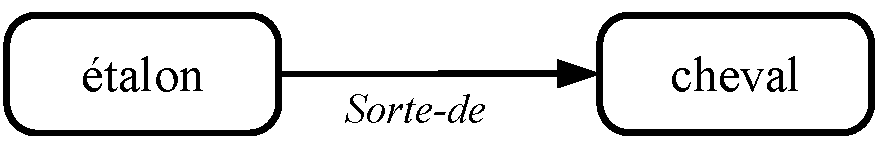
\includegraphics[height =
    1cm]{2_Etat-art/img/ReseauxSemantiquesElemA}} \centering \subfigure[On
  rajoute un n\oe ud au réseau pour indiquer que Tornado est un
  étalon]{
\includegraphics[height = 1cm]{2_Etat-art/img/ReseauxSemantiquesElemB}}

  \caption{Réseaux sémantiques élémentaires.}\label{fig:ReseauxElem}
\end{figure}

On constate sur l'exemple \ref{fig:ReseauxElem} que la représentation
des deux premières informations (\sentence{Un étalon est un cheval} et
\sentence{Tornado est un étalon}) permet de déduire facilement par
transitivité que \sentence{Tornado est un cheval}.\\

%\subparagraph{Composition de relations}

L'exemple précédent présente une composition entre deux relations.  Il
est possible de retrouver les informations contenues dans le graphe
par simple \emph{héritage des propriétés} en suivant les arcs
\emph{Sorte-de}.  Cette composition des relations %est la transposition
%dans les réseaux sémantiques du principe d'économie abordé à la
%section \ref{sec:reseaux-semantiques}, il 
permet de réaliser une
économie d'espace mémoire pour la représentation du réseau mais
ralentit le temps de traitement. %Pour Quillian, cognitivement, la
%longueur du chemin reliant deux n\oe uds doit refléter le temps mis
%par des humains pour associer les concepts correspondant à ces n\oeuds et leurs propriétés.  
Le réseau de la figure
\ref{fig:heritageProprietes} permet de retrouver que les
\emph{étalons} en général et \emph{Tornado} en particulier possèdent
des \emph{sabots}. 


\begin{figure}[htbp]
  \centering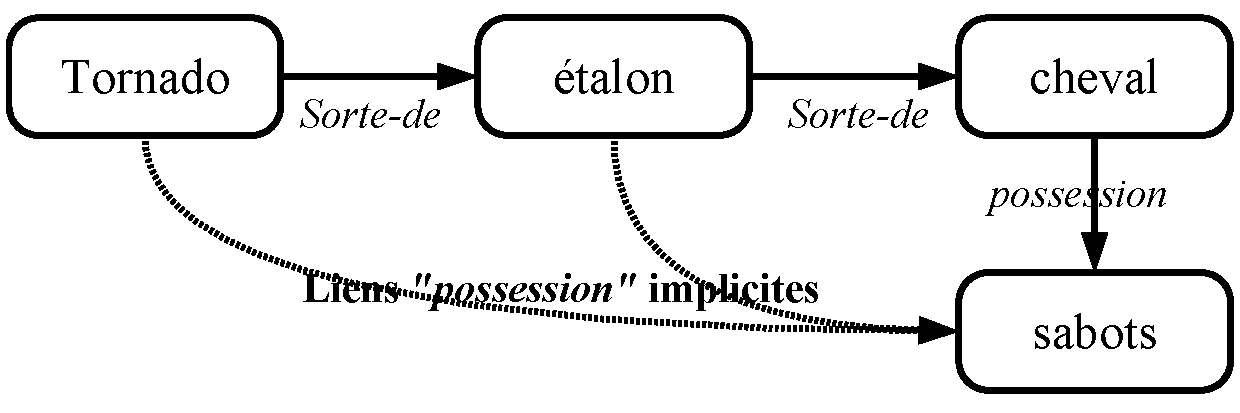
\includegraphics[height = 3cm]{2_Etat-art/img/HeritageProprietes}

 \caption{Héritage de propriétés}\label{fig:heritageProprietes}
\end{figure}


Tous les raisonnements sur le réseau peuvent être modélisés par une
\emph{table de composition des relations} qui contient l'ensemble des
compositions autorisées dans le réseau et leurs relations résultantes
respectives. Par exemple, le réseau de la figure
\ref{fig:heritageProprietes} contient la propriété
{\emph{Sorte-de}~$\circ$~\emph{possession}~$=$~\emph{possession}. \\

% \begin{figure}[htbp]
   %\centering \subfigure[Représentation erronée des informations dans
   %un réseau]{ 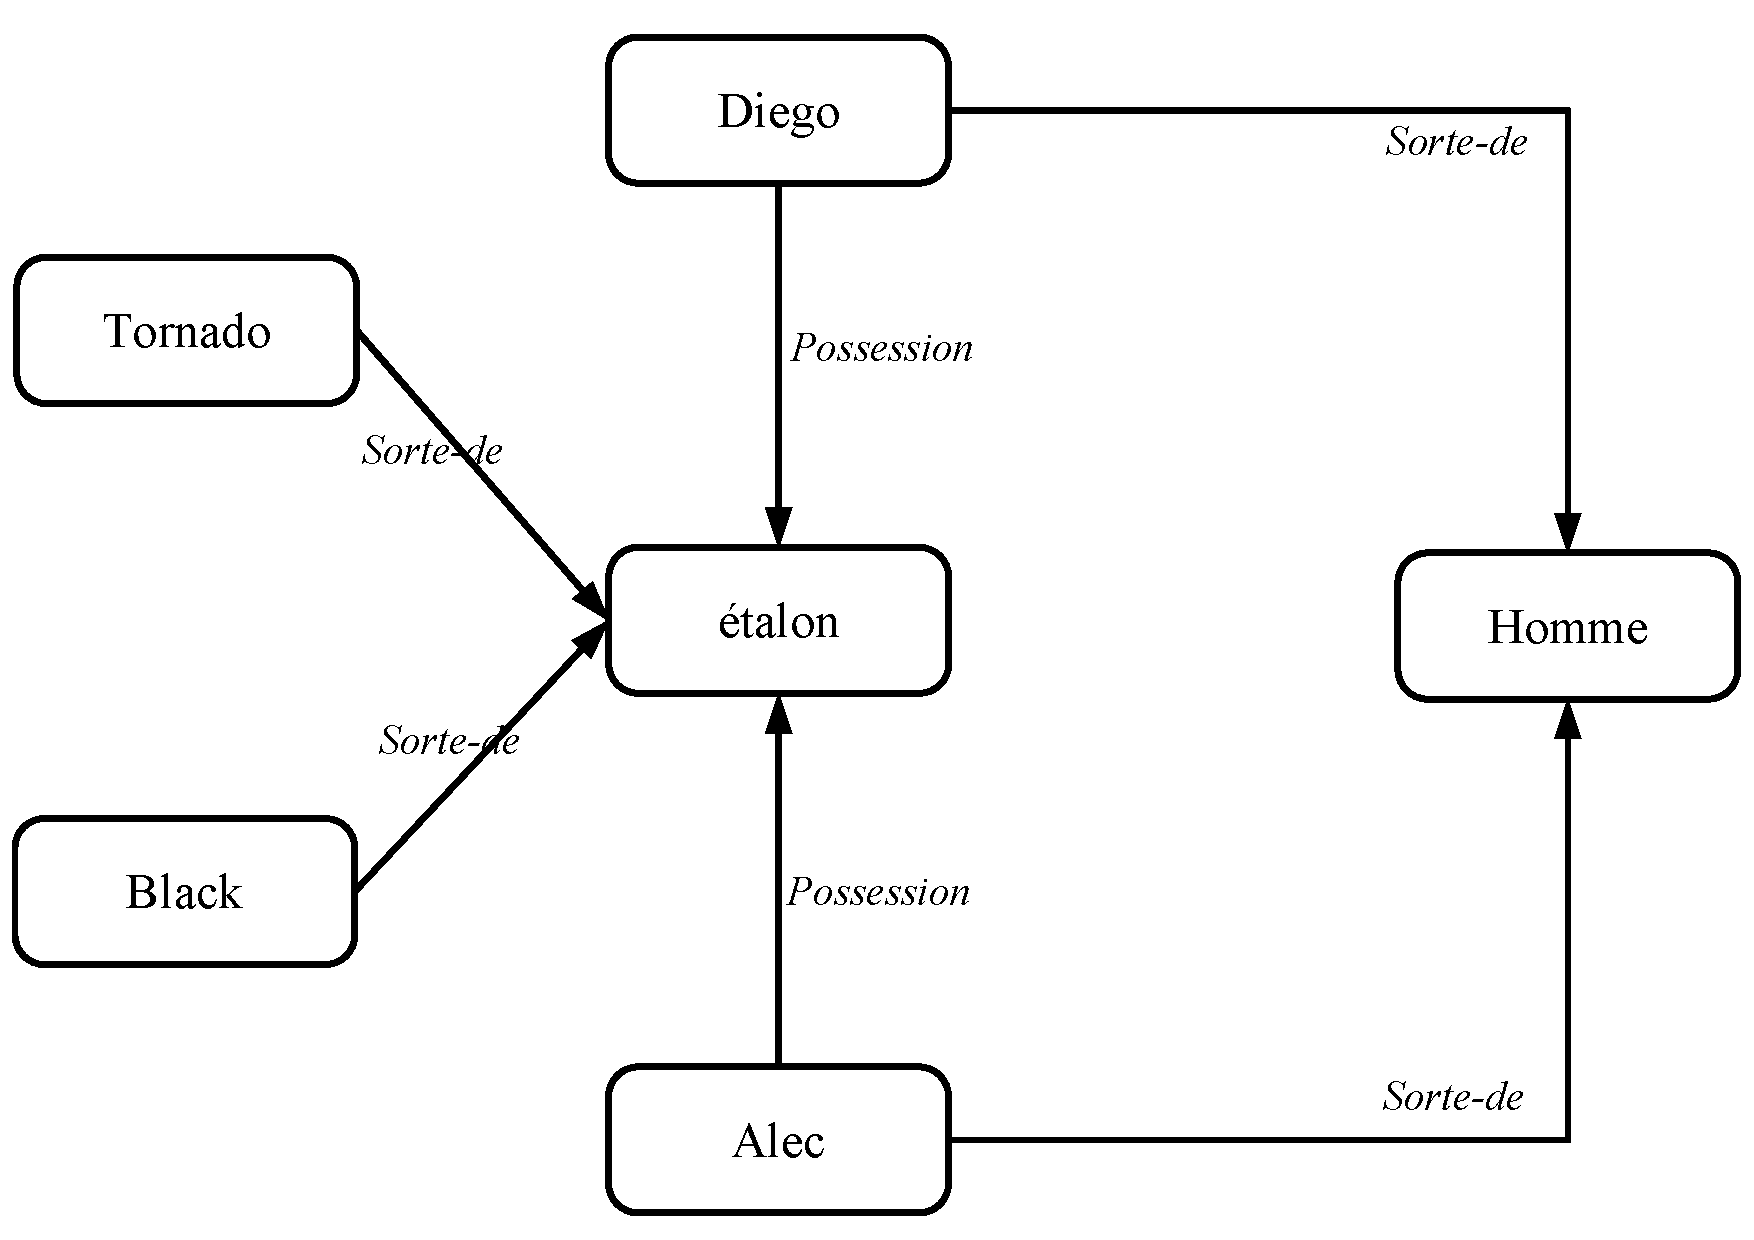
\includegraphics[width = 6.5cm]{2_Etat-art/img/ambiguiteReseau}
    %\label{fig:ambiguiteReseau}} \hskip 1cm \centering
  %\subfigure[Représentation correcte des informations de la
  %figure]{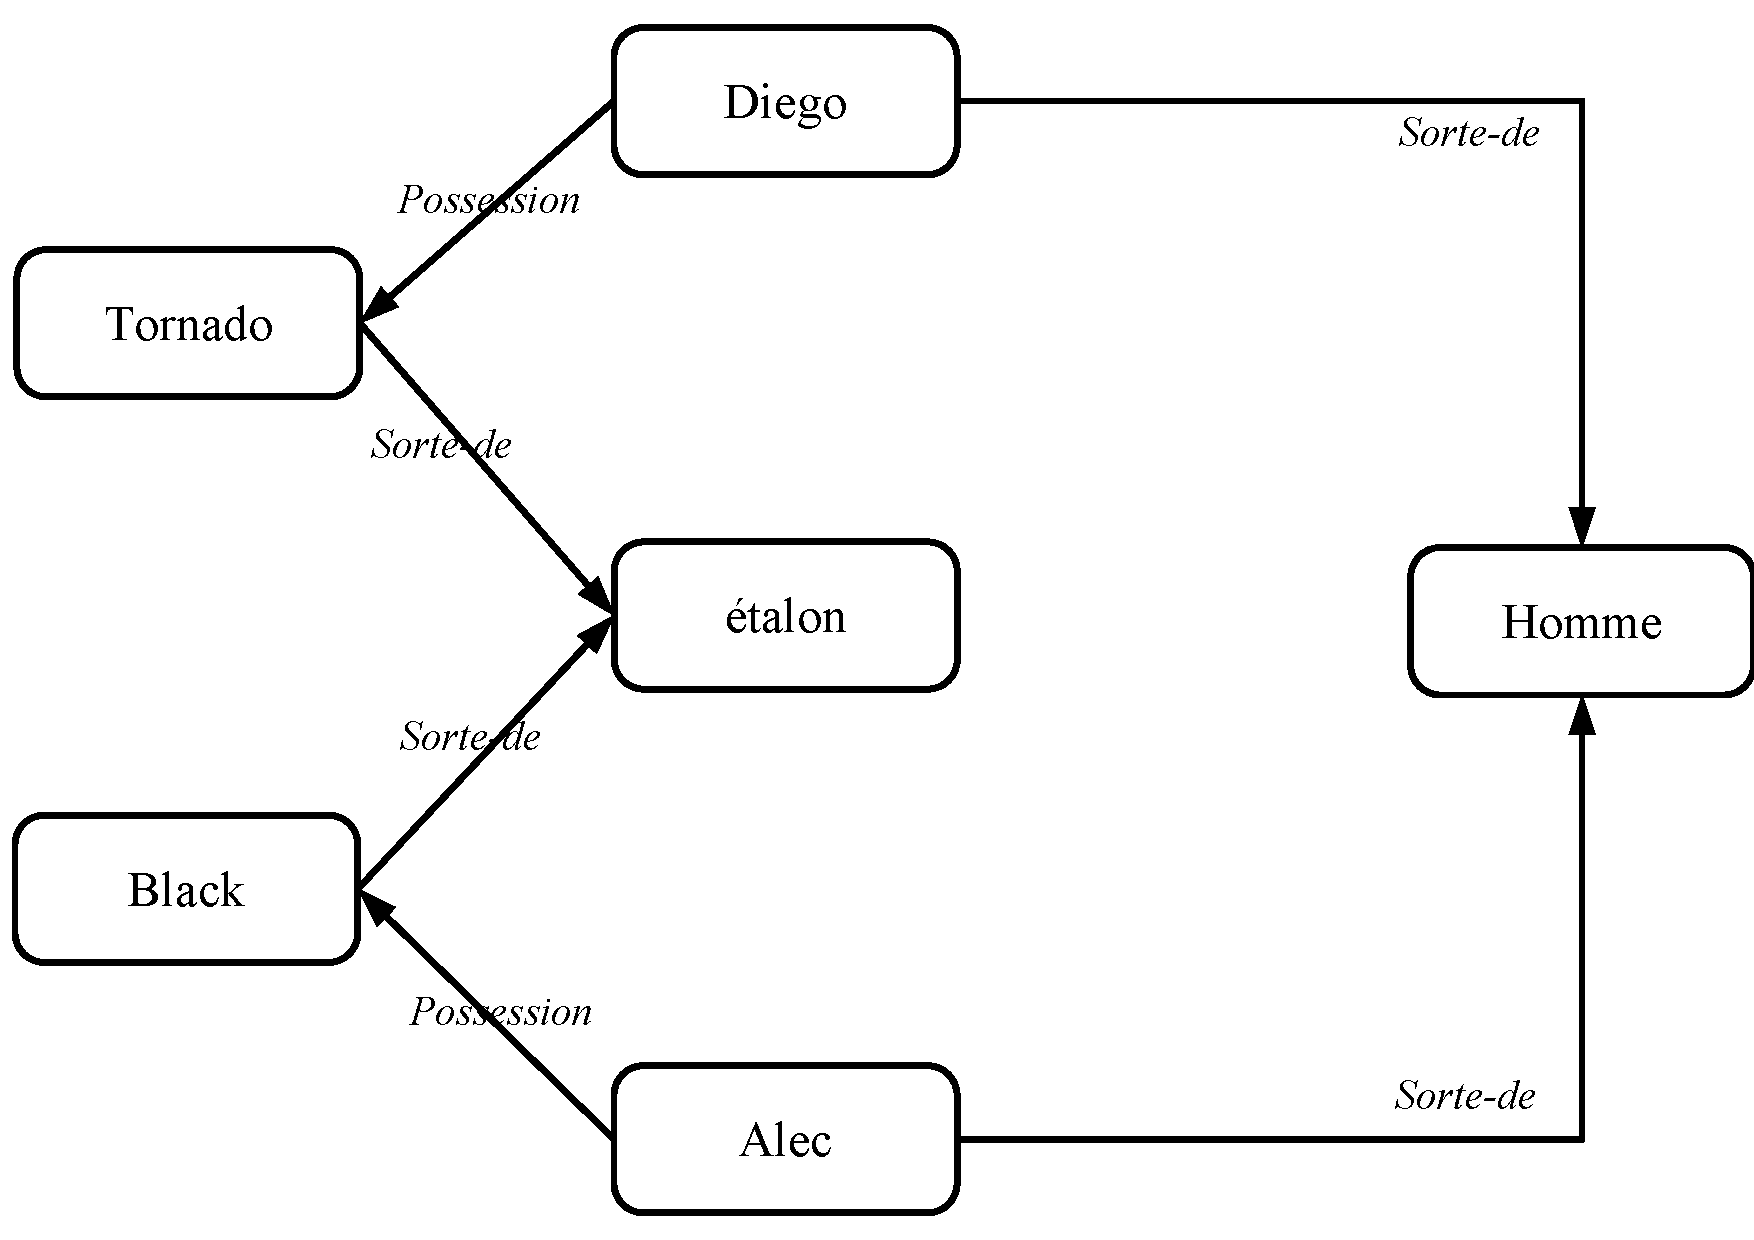
\includegraphics[width =
   % 6.5cm]{2_Etat-art/img/correctionAmbiguiteReseau}\label{fig:correctionAmbiguiteReseau}}
   %\caption{Importance de la différenciation des types de n\oe uds dans
    % un réseau sémantique \label{fig:ambReseau}}
%\end{figure} 

%\subparagraph{Types de n\oe ud}

%Représenter une information comme \sentence{Diego possède un étalon}
%peut poser le problème de l'arc à introduire dans le réseau. Il ne
%faut pas comme sur le réseau de la figure~\ref{fig:ambiguiteReseau}
%mettre un arc de \emph{Possession} entre les n\oe uds \emph{Diego} et
%\emph{cheval} puisque cela signifierait que l'ensemble des éléments de
%la catégorie \emph{cheval} appartient à \emph{Diego}. La
%représentation correcte verrait un arc entre un propriétaire et une
%instance de la classe \emph{cheval}, dans l'exemple
%\ref{fig:correctionAmbiguiteReseau} pour \emph{Diego}, \emph{Tornado}
%et pour \emph{Alec}, \emph{Black}. Il est donc nécessaire de
%différencier les n\oe uds d'instance des n\oe uds de classes.

%On veut aussi pouvoir représenter d'autres informations comme des
%informations temporelles (\sentence{Alec possède Black d'octobre 1941
  %à août 1950}) auquel cas l'état n'est plus simplement codé par un
%lien mais aussi par un n\oe ud. Ce n\oe ud sera alors une
%spécialisation de la notion d'\emph{appartenance} comme le montre la
%figure \ref{fig:EtatCodeNoeud}

%\begin{figure}[h]
 % \centering 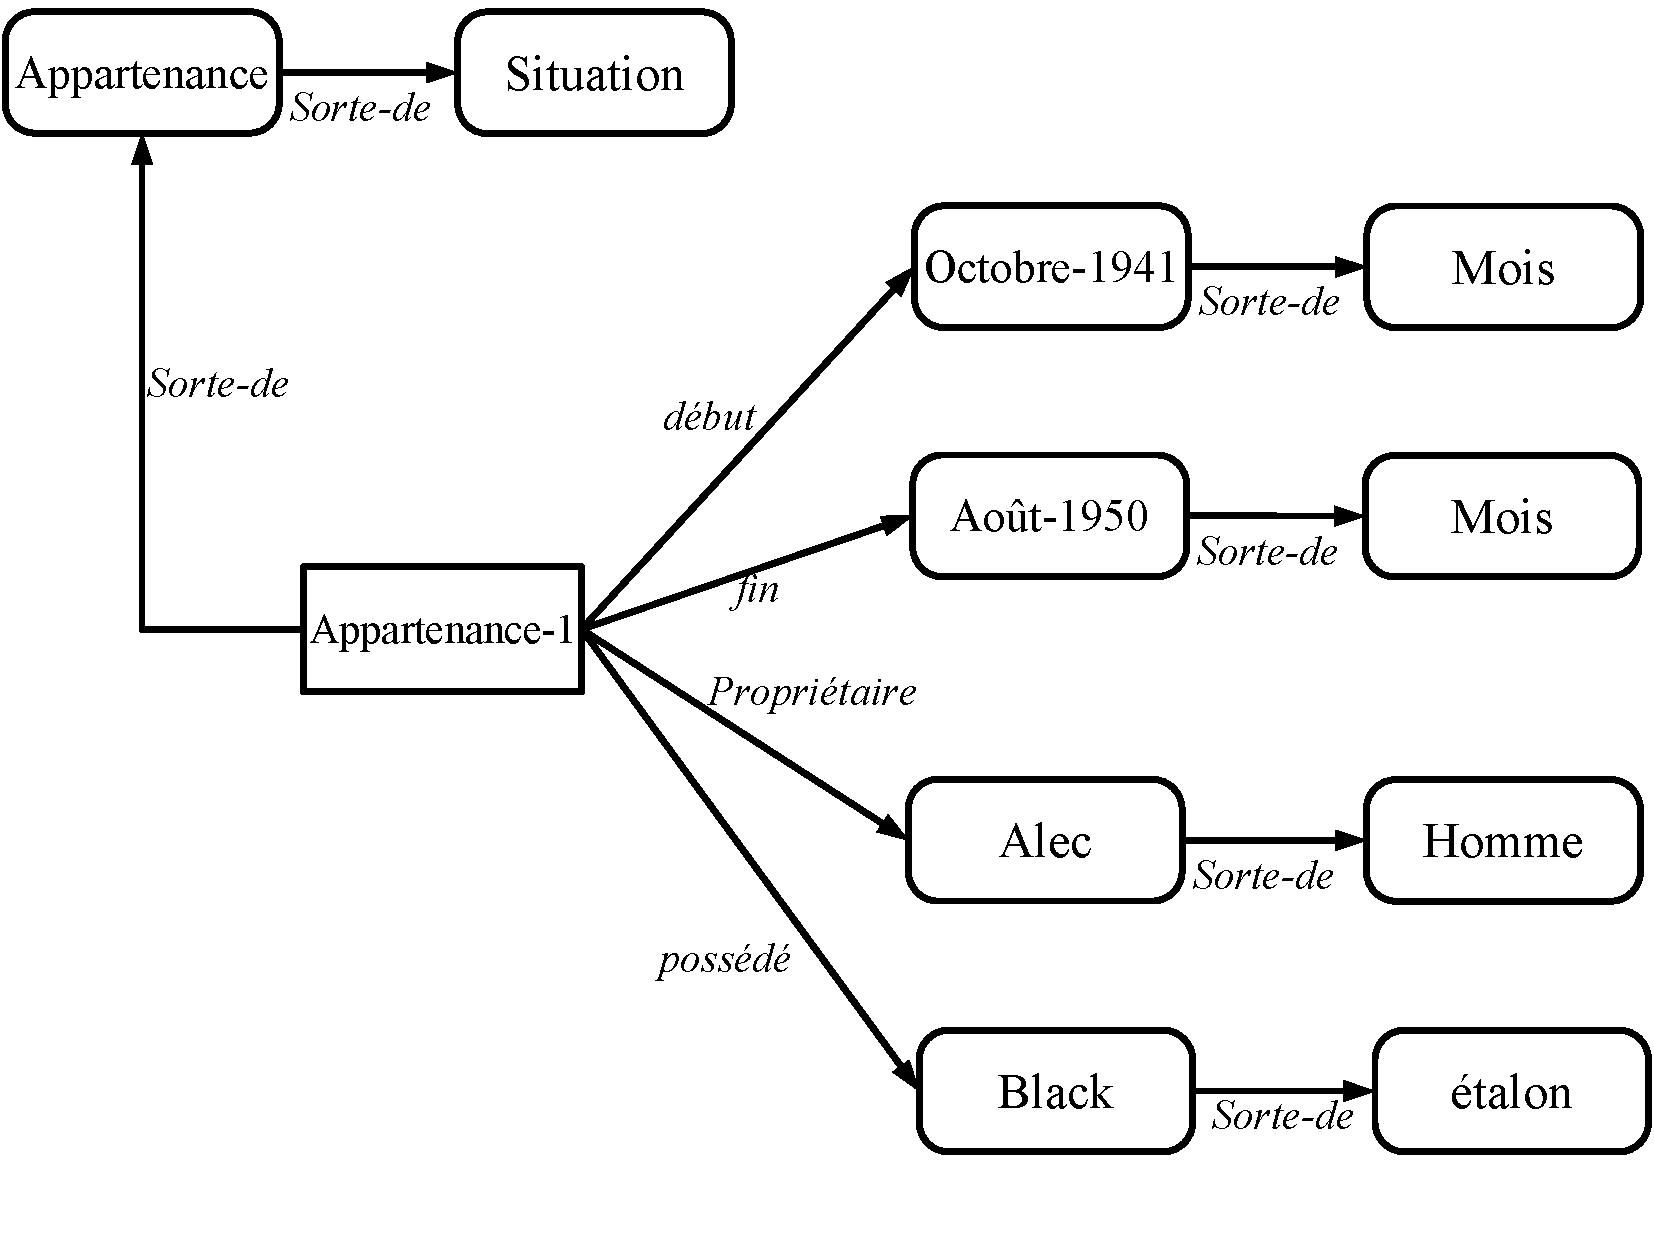
\includegraphics[width = 9cm]{2_Etat-art/img/EtatCodeParNoeud}

 %\caption{Représentation de l'information \sentence{Alec possède Black
    % d'octobre 1941 à août 1950}\label{fig:EtatCodeNoeud}}
%\end{figure}

Dans la famille des réseaux sémantiques, il convient de citer les
\emph{graphes conceptuels} (GC) \cite{Sowa1984}
\cite{Sowa2000}\footnote{Une pré-version de cet ouvrage est disponible
  en ligne à l'adresse \url{http://www.jfsowa.com/krbook/index.htm}}.
Un GC est un graphe biparti étiqueté dont les deux classes de sommets
correspondent à des \emph{concepts} et des \emph{relations
  conceptuelles} entre ces concepts.  La figure \ref{fig:exemple_GC}
présente un exemple de graphe conceptuel avec la phrase \sentence{John
  va à Boston en bus.}.  L'avantage principal qu'offrent les GC est
que le modèle est muni d'une sémantique en logique du premier ordre
qui est adéquate et complète par rapport à la déduction.  Les
applications des graphes conceptuels concernent, entre autres, la
génération automatique de langage \cite{Nogier1991} ou la recherche
d'informations \cite{Genest2000}.


\begin{figure}[htbp]
  \centering 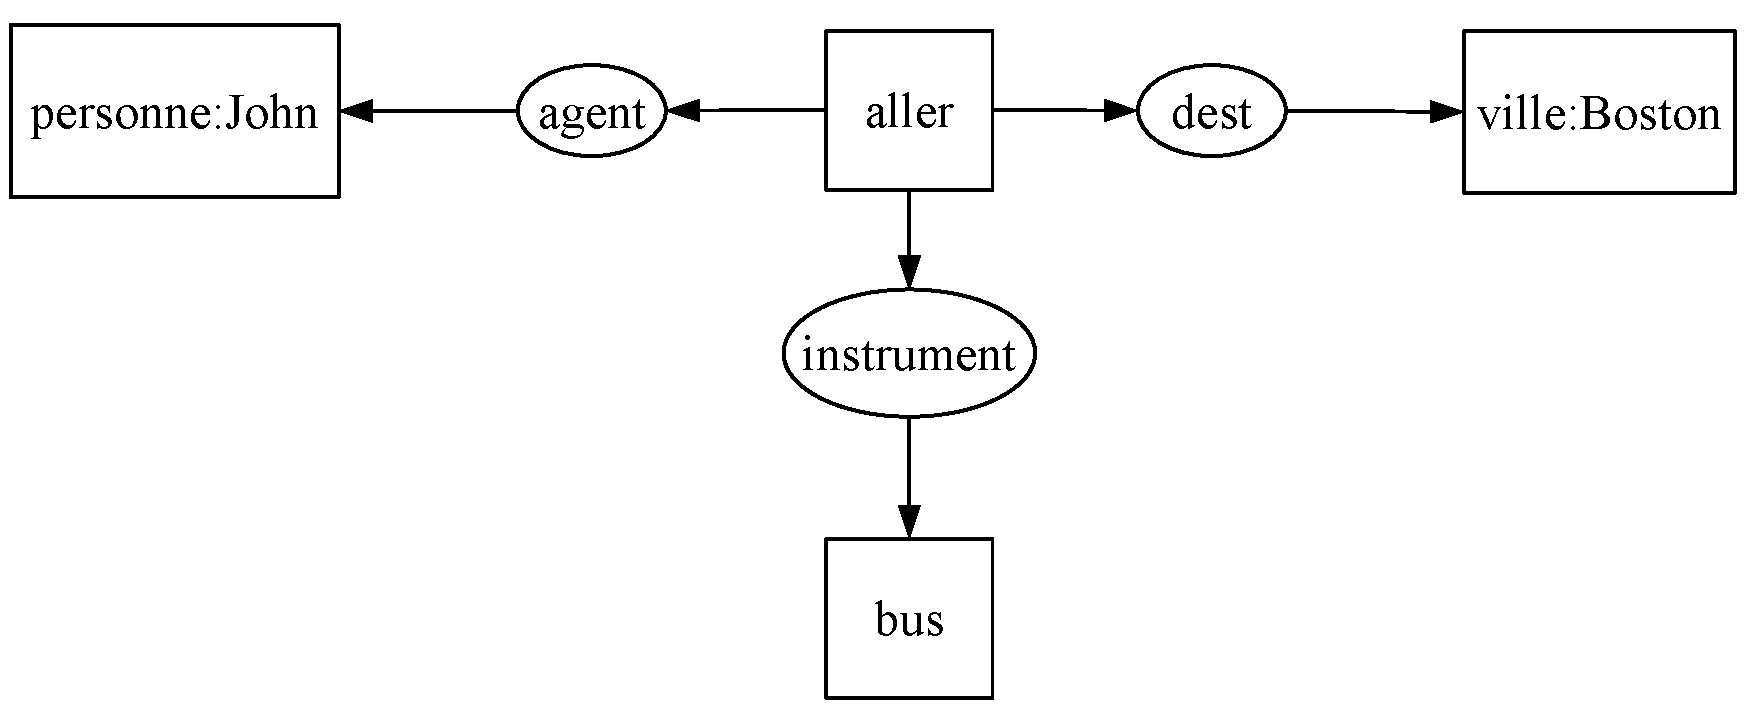
\includegraphics[width = 10cm]{2_Etat-art/img/exemple_GC}

  \caption{Exemple de graphe conceptuel : \sentence{John va à Boston
      en bus.}\cite{Sowa2000}}\label{fig:exemple_GC}
\end{figure}

\subsubsection{Les réseaux d'aujourd'hui : WordNet}

%Contrairement aux réseaux sémantiques classiques qui cherchent à la
%fois à représenter des phrases et à ordonner les connaissances sur le
%monde (le côté ontologique des réseaux), le projet WordNet est
%uniquement concentré sur cette deuxième tâche. Libre ensuite aux
%développeurs de l'utiliser pour d'autres applications. 
WordNet est une
base de données lexicale pour l'anglais développée sous la direction
de George Armitage Miller \born{1920} par le \emph{Cognitive Science
  Laboratory} de l'université de Princeton (\'Etats-Unis d'Amérique).
Il se veut représentatif du fonctionnement de l'accès au lexique
mental humain.

WordNet est organisé en ensembles de synonymes appelés synsets. À
chaque synset correspond un concept. Le sens des termes est décrit
dans WordNet par trois moyens :

\begin{itemize}
  
\item leur \emph{définition}
  
\item le \emph{synset} auquel ce sens est rattaché.
  
\item les \emph{relations lexicales} qui unissent entre eux les
  synsets.  Ces relations sont ici l'hyperonymie, la méronymie ainsi
  que l'antonymie.

\end{itemize}

La version 3 de WordNet\footnote{Voir \url {http://wordnet.princeton.edu/wordnet/man/wnstats.7WN.html}.} compte 155287 termes ce qui constitue une
couverture relativement large de la langue anglaise. Les relations
lexicales présentes dans WordNet ne connectent que les termes de même
morphologie. %(il n'y a pas de relations comme la substantification $S_0$ cf. \ref{sec:fonct-lexic-de-prod}). 
Il y a donc une hiérarchie
pour les noms, une pour les adjectifs, une pour les verbes et enfin
une dernière pour les adverbes. Un extrait de la hiérarchie des noms
est présenté dans la figure \ref{fig:wordnet}.

\begin{figure}[htbp]
  \centering 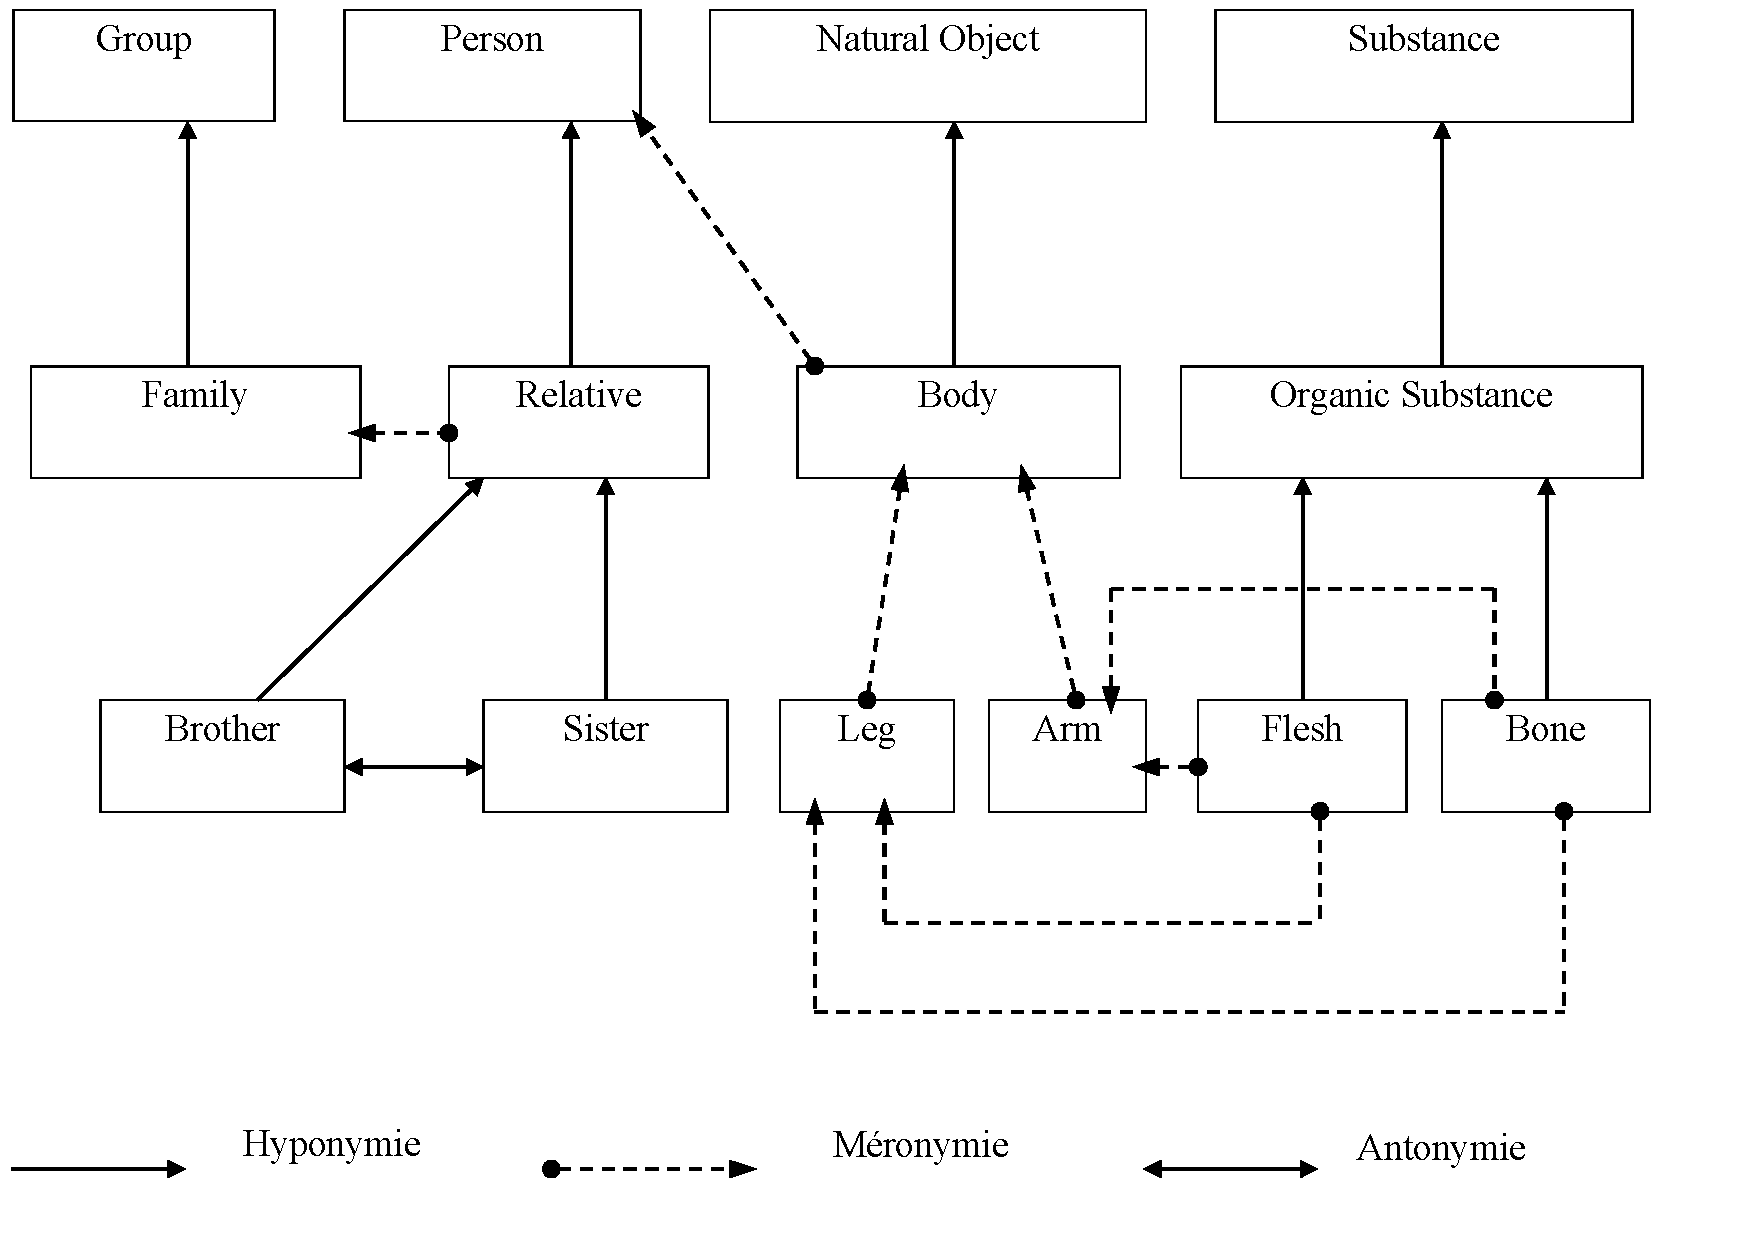
\includegraphics[width = 10cm]{2_Etat-art/img/wordnet}

  \caption{Extrait de la hiérarchie des noms}\label{fig:wordnet}
\end{figure}

Dans \cite{Harabagiu1999}, les auteurs de \emph{WordNet} (alors à sa
version 1.6) relèvent six faiblesses dans la construction de leur
réseau : (1)~le manque de liens entre les hiérarchies; (2)~le nombre
limité de relations entre termes traitant du même sujet; (3)~le manque
de relations morphologiques; (4)~l'absence de relations thématiques;
(5)~l'absence de certains sens de mots; (6)~le manque d'uniformisation
et de cohérence dans les définitions.  Si les points 3, 5 et 6 ne nous
intéressent pas dans cet article, nous allons montrer l'apport des
vecteurs conceptuels pour la résolution des autres, tous trois formant
le problème du tennis.


%\paragraph{Limites des réseaux sémantiques}

%L'une des principales critiques adressées aux réseaux sémantiques
%concerne le modèle de la mémoire associative dont ils sont issus. En
%effet, diverses études ont montré que certains hyponymes sont plus
%caractéristiques de leur catégorie que d'autres.  Par exemple, une
%\lexItem{pomme} ou une \lexItem{orange} sont plus considérées comme
%appartenant au genre \lexItem{fruit} qu'une \lexItem{noix} ou une
%\lexItem{olive} si on se réfère aux temps de réaction des sujets. Par
%ailleurs, Carol Conrad~\cite{conrad1972} a montré que les temps de
%réaction des sujets à des énoncés n'étaient pas seulement fonction du
%nombre d'individus de la classe et du parcours d'un réseau
%d'hyponymes, mais aussi de la fréquence des énoncés (cf.
%figure~\ref{fig:temps_reaction_conrad}).

%\begin{figure}[htbp]
 %\begin{tabular}{|c|c|c|}
    %\hline
    %niveau&fréquent&rare\\
    %\hline
     %1&\sentence{Un requin peut bouger}&\sentence{un saumon a une bouche}\\
    %2&\sentence{Un oiseau peut bouger}&\sentence{Un poisson a des yeux}\\
    %3&\sentence{Un animal peut bouger}&\sentence{Un animal a une peau}\\
   % \hline
  %\end{tabular}
  %\centering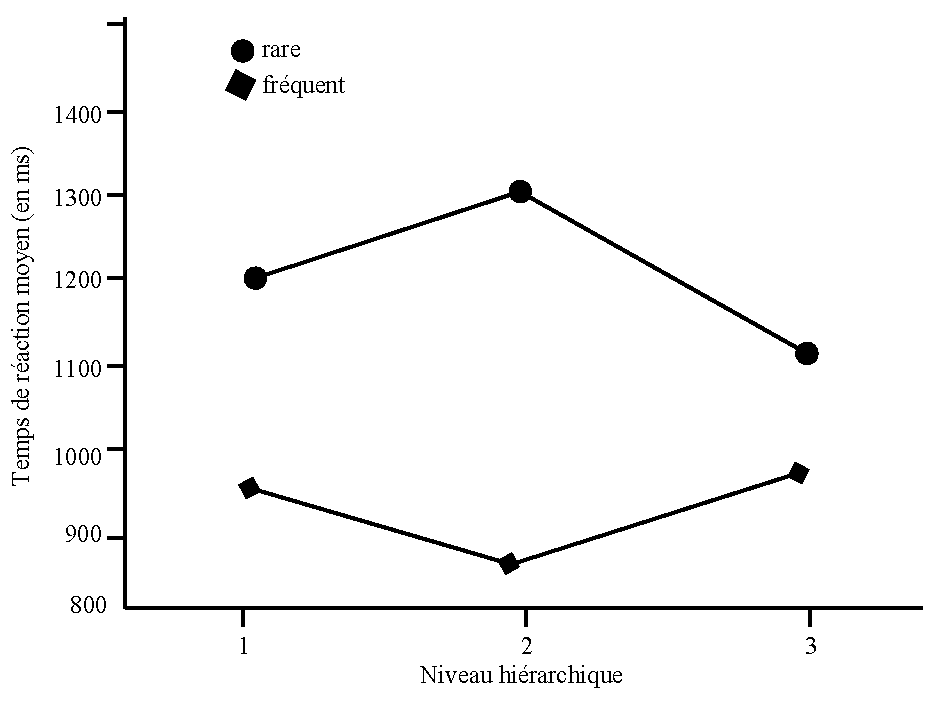
\includegraphics[width=10cm]{2_Etat-art/img/temps_reaction_conrad}

 %\caption{Expérience de Conrad
   %\cite{conrad1972}}\label{fig:temps_reaction_conrad}
%\end{figure}

%Ces remarques sont à la base de la \emph{sémantique du prototype} dont
%les tenants considèrent que chaque classe contient un prototype,
%c'est-à-dire un élément plus "typique" que les autres (la
%\lexItem{pomme} pour les fruits par exemple); en d'autres termes,
%qu'il présente dans sa catégorie \sentence{à la fois un maximum de
  %points communs avec les autres éléments de la catégorie et un
 % minimum de points communs avec les éléments de catégories opposées}
%\cite{Nyckees1998}.

%Comme nous l'avons dit dans la partie \ref{sec:an-prod-textes},
%l'adéquation avec le modèle cognitif ne suffit pas à justifier que ce
%modèle informatique est insuffisant. Celui-ci est aussi l'objet de
%critiques de fond, en particulier de la part de François Rastier
%\cite{Rastier2004}. Il lui reproche de n'être qu'une vision du monde.
%\sentence{Ce qu'on appelle le mobilier ontologique du monde, ce qui
  %est présenté comme naturel et dit par toutes les langues appartient
  %en réalité à un certain type de civilisation}. Certaines langues
%distinguent \lexItem{pied} et \lexItem{jambe}, ce que les langues
%slaves ou malaises ne font pas.

%Les réseaux sont utilisés comme si les sens étaient prédéterminés or
%ce n'est pas le cas. Il y a des coutumes d'usage mais les langues
%évoluent et ses coutumes aussi. Certains termes sont créés
%(néologismes), d'autres prennent de nouvelles acceptions, certaines de
%ces formations devenant plus fréquentes se verront lexicaliser et
%finalement figurer dans un dictionnaire. Dans le cas des réseaux,
%\sentence{on fixe (la langue), on la bloque dans un moment, dans une
  %forme de civilisation ou du moins dans une forme de système
  %économico-technique et on dit voilà ce que c'est que l'esprit
  %humain. \c{C}a s'appelle une prise de pouvoir.}\footnote{Extrait de
  %l'émission \emph{Tire ta langue} du 18 Février 2003 sur \emph{France
   % Culture}
  %\url{http://www.radiofrance.fr/chaines/france-culture2/emissions/tire_langue/fiche.php?diffusion_id=11608}}

%\subsubsection{Bases d'acceptions}

%Le modèle de base d'acceptions a été développé à Grenoble %depuis le début des années 1990 
%par Gilles Sérasset \index{Sérasset Gilles} et
%Christian Boitet \index{Boitet Christian}.  Aujourd'hui, sa principale
%implémentation concerne le projet Papillon dont elle constitue la
%macrostructure. Ce projet, mené depuis 2000, vise à la constitution
%d'une base lexicale multilingue linguistiquement riche. Du côté
%organisationnel, son principal atout est de se baser sur un principe
%collaboratif qui permet à n'importe quelle personne qui le souhaite de
%l'enrichir \cite{Mangeot2003}. La base comprend entre autres
%l'anglais, le français, le japonais, le malais, le lao, le thaï, le
%vietnamien et le chinois. \\

%%\paragraph{Acceptions} \label{sec:acceptions}

%Une acception est un sens particulier d'un mot, admis et reconnu par
%l'usage.  Il s'agit d'une unité sémantique propre à une langue donnée
%\cite{Serasset2001}. Par exemple, en français, l'item lexical
%\lexItem{bague} a, au moins, deux acceptions, l'\annotation{anneau},
%ou la collerette de papier entourant le cigare (annotée
%\annotation{cigare}) tandis que l'item lexical \lexItem{sonnerie} en a
%deux, le \annotation{son} et le \annotation{mécanisme} qui l'émet. Une
%acception est en fait ce qu'on appelle communément \sentence{un sens
%  d'un mot}.  Ainsi, pour revenir à l'une de nos préoccupations
%principales, désambiguïser, c'est trouver quelle est l'acception d'un
%mot qui semble concorder le mieux avec les autres mots de la phrase. \\

%%\paragraph{Base d'acceptions}\label{sec:base-dacceptions}

%Une base d'acceptions monolingue contient des entités \lexobj{item
%  lexical} et des entités \lexobj{acception} qui regroupent les
%informations sur les différents sens que peut prendre l'item. %Dans le
%%cas du dictionnaire Papillon, par exemple, cette microstructure est
%%basée sur la Lexicographie Explicative et Combinatoire, partie de la
%%Théorie Sens-Texte (cf \ref{sec:fonct-lexic-de-prod}).

%%La figure \ref{item-acception-bague-sonnerie} présente l'architecture
%%d'une base par acception avec \lexItem{bague} et \lexItem{sonnerie}
%%dans un cadre monolingue. Les acceptions ont été annotées pour
%%faciliter la compréhension.

%%\begin{figure}%[H]
%  
%  %\centering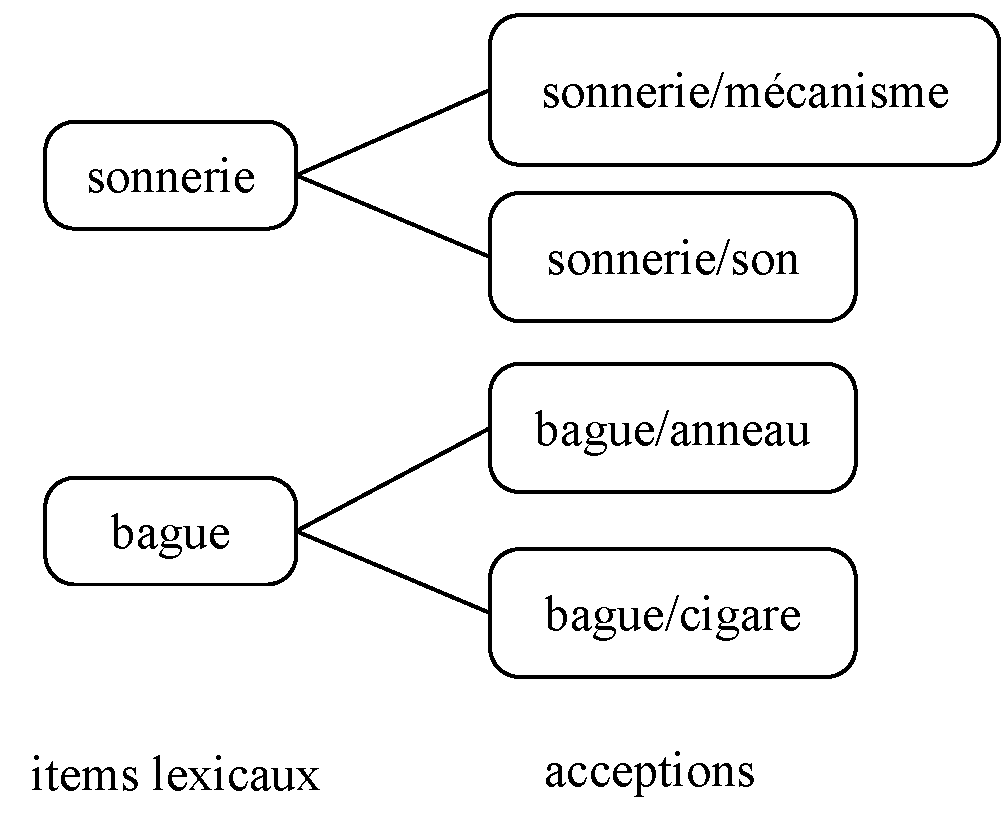
\includegraphics[height =
%  %6cm]{2_Etat-art/img/acception-bague-monolingue}
%    %\caption{Items lexicaux et acceptions de \lexItem{bague} et
%      %\lexItem{sonnerie}}\label{item-acception-bague-sonnerie}
%%\end{figure}

%Dans un cadre multilingue \cite{Mangeot2003}, une base contient
%plusieurs bases d'acceptions monolingues dont les acceptions sont
%reliées par des acceptions interlingues appelées \emph{axies}. Un
%exemple d'une telle architecture est présenté en
%\ref{item-acception-bague-sonnerie-inter}.  D'un côté les acceptions
%monolingues du français, de l'autre celles de l'anglais reliées entre
%elles par des axies.

%\begin{figure}%[H]
%  
%  \centering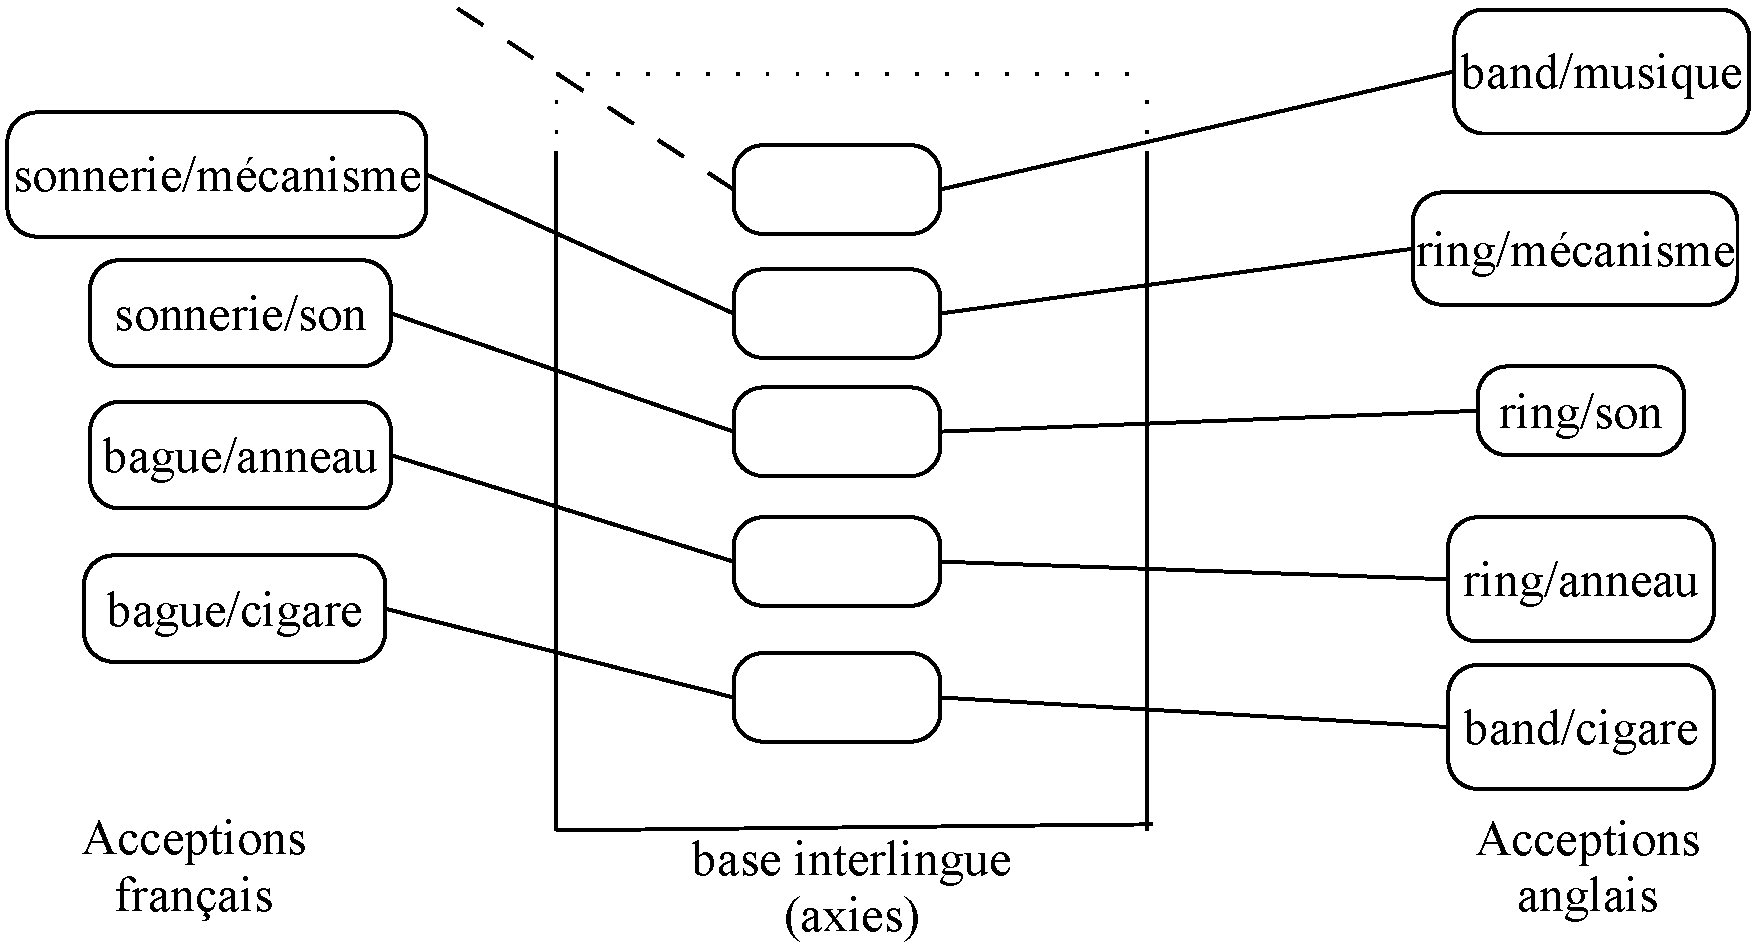
\includegraphics[height = 6cm]{2_Etat-art/img/acception-bague-multilingue}
%    \caption{Acceptions et axies en
%      multilingue}\label{item-acception-bague-sonnerie-inter}
%\end{figure}

%Ce système permet de représenter les raffinements de sens de certaines
%langues. L'exemple de \lexItem{fleuve} et \lexItem{rivière} est
%caractéristique. Le français différencie, en effet, \sentence{un cours
%  d'eau qui se jette dans la mer ou l'océan.} (\lexItem{fleuve}) et
%\sentence{cours d'eau qui se jette dans un autre cours d'eau}
%(\lexItem{rivière}) tandis que ni l'anglais ni l'espagnol ne font
%cette distinction (cf.figure \ref{acception-raffinement-riviere}).

%\begin{figure}[H]
%  
%  \centering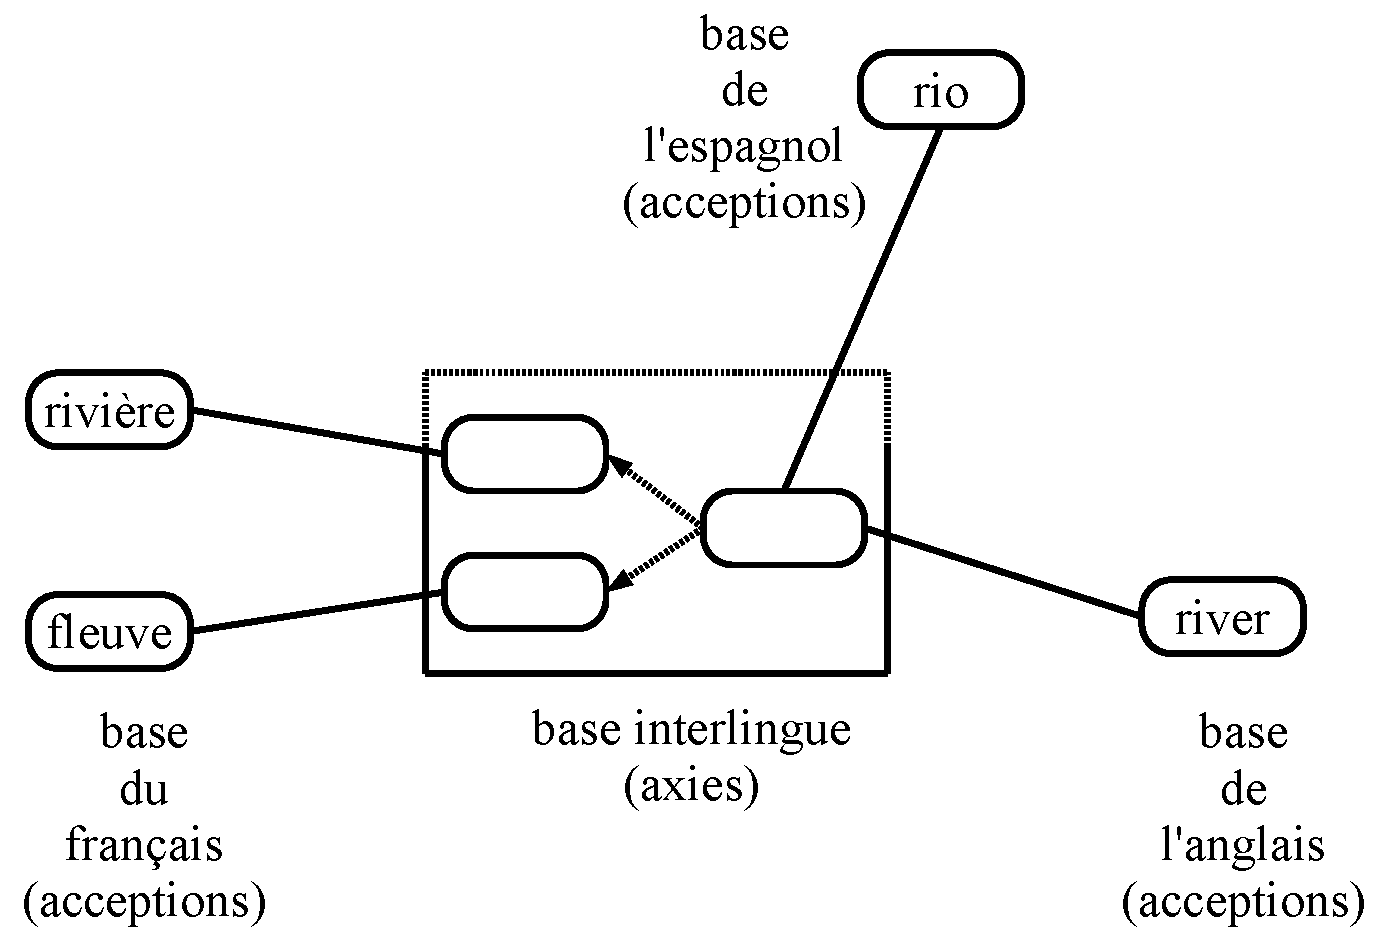
\includegraphics[height =
%  8cm]{2_Etat-art/img/acception-rafinement-riviere}
%    \caption{Exemple de raffinement de
%      sens.}\label{acception-raffinement-riviere}
%\end{figure}

\subsection{Approche componentielle (ou sémique)}\label{sec:appr-componentielle}

\subsubsection{Le sens vu comme la composition de primitives}
\label{sec:sens-vu-primitives}

La linguistique componentielle postule que le sens d'un terme peut
être défini par un ensemble d'éléments de sens plus petits, appelés, suivant les
diverses écoles, sèmes, noèmes, traits
sémantiques, atomes de sens, primitives de base\ldots 
La linguistique componentielle tire son origine des années 1940 et des
travaux de Hjelmslev \cite{Hjelmslev1968} sur l'analyse en composants sémantiques (comparaison des termes en fonction des sèmes qui les composent).

L'analyse sémique s'attache à identifier pour un certain nombre de
termes l'ensemble des sèmes qu'ils
comportent.  Même si ces sèmes ne sont pas des atomes de
sens, mais des traits distinctifs, ils supposent
l'existence dans l'esprit humain de primitives de sens, les sèmes n'en
étant alors que des compositions s'opposant entre elles.  Ainsi,
contrairement à la distributionnalité présentée en
\ref{sec:appr-distr} qui est une théorie purement linguistique et qui
donc ne repose pas sur un postulat cognitif, il s'agit ici de
comprendre comment les mots coexistent dans notre esprit
\citep{Nyckees1998}{216}.

Parmi les analyses sémiques les plus connues figurent celles
effectuées par Bernard Pottier \cite{Pottier1964}. La figure
\ref{fig:an-sem-Pottier} présente l'analyse sémique de certains
véhicules. Les signes + et - marquent la présence ou l'absence du
trait tandis que \~{} spécifie que le trait est indifférent.

\begin{figure}%[H]
\begin{center}
%\begin{tabular}{p{2cm} p{1.8cm} p{1.8cm} p{1.8cm} p{1.8cm} p{1.8cm} p{1.8cm}}
  {\fontsize{10}{11}\selectfont
  \begin{tabular}{|c|c|c|c|c|c|c|c|c|c|}
\hline
%&&&&&&&&&\\
& sur & sur & deux & individuel & payant & 4 à 6 & intra- & transport
& transport de \\ & terre & rail & roues & & & personnes & urbain &
d'objets & personnes\\
 %&&&&&&&&&\\
\hline voiture&+&-&-&+&-&+&\~{}&\~{}&+\\ \hline
taxi&+&-&-&\~{}&+&+&\~{}&\~{}&+\\ \hline
autobus&+&-&-&-&+&-&+&\~{}&+\\ \hline autocar&+&-&-&-&+&-&-&\~{}&+\\
\hline métro&+&+&-&-&+&-&+&\~{}&+\\ \hline
train&+&+&-&-&+&-&-&\~{}&+\\ \hline avion&-&-&-&\~{}&+&\~{}&-&\~{}&+\\
\hline moto&+&-&+&+&-&-&\~{}&\~{}&+\\ \hline
bicyclette&+&-&+&+&-&-&\~{}&\~{}&+\\ \hline
\end{tabular}
}
\end{center}
\caption{Analyse sémique des véhicules selon Pottier}
\label{fig:an-sem-Pottier}
\end{figure} 

Par ailleurs, les primitives de sens doivent permettre d'exprimer la signification
de tout énoncé quelle que soit la langue dans laquelle il est exprimé.
Ainsi, dans la théorie atomiste, les primitives sémantiques sont
nécessairement universelles et surtout elles sont à la fois
\emph{indépendantes} et \emph{antérieures} au langage. Ainsi, elles
devraient nécessairement se retrouver présentes dans toutes les
langues.

\paragraph{Limites de l'approche componentielle}
\subparagraph{Chez les linguistes}\label{sec:chez-les-linguistes}

À la suite d'études approfondies sur les langues les plus diverses
durant presque trente ans, une liste
de 35 primitifs universaux  a été présentée \cite{Wierzbicka1993}.
Le principal problème posé par cette liste est que, là où on simplifie
les choses en présentant un nombre fort restreint de primitives, on
augmente singulièrement la difficulté de représenter le sens d'un
terme. Un deuxième problème concernant cette vision est son
caractère utopique. En effet, la notion ne rentre dans les primitifs
que si elle est universelle donc si elle est présente dans l'ensemble
des langues du monde. Or du fait de leur grand nombre (environ 6000), cette étude semble particulièrement difficile à
réaliser. Pour cette raison purement pratique, on ne pourra donc
jamais être totalement certain de l'universalité d'un concept.

\subparagraph{Chez les informaticiens}

Les créateurs des systèmes informatiques des années 1970 comme Schank
\cite{schank1972} et Wilks sont directement héritiers de l'analyse
sémique et à ce titre, ils cherchent principalement quelles primitives
permettraient de représenter l'ensemble des sens en langue. Ainsi,
Yorick Wilks énonce quelques critères très généraux pour fabriquer un
ensemble de primitives \cite{Wilks1977} :

\begin{enumerate}
  
\item \emph{finitude} : l'ensemble de primitives doit être fini et de
  relativement faible dimension. En particulier, cette dernière doit
  être très largement inférieure au nombre de sens à décrire ;
  
\item \emph{étendue} : les primitives doivent couvrir l'ensemble de
  l'intervalle des sens à exprimer ;
  
\item \emph{complétude} : toutes les informations sur le sens d'une
  entité doivent pouvoir être décrites grâce à l'ensemble de
  primitives ;
  
\item \emph{canonicité} : la description d'une entité doit être unique
  et non-ambiguë ;
  
\item \emph{indépendance} : aucune primitive ne doit pouvoir être
  décomposable en un ensemble d'autres ;
  
\item \emph{non-réductibilité} : l'ensemble de primitives ne peut être
  remplacé par un ensemble plus petit.

\end{enumerate}

%\begin{figure}%[H]
 % \begin{tabular}{p{1.5cm}|c|c|c|} 
%\cline{2-4}
%&classe&nombre&exemples\\
%\cline{2-4}
%&entités&19& \cname{humanité}, \cname{substance}, \cname{objet physique}\\
%\cline{2-4}
%&actions &34&\cname{causer}, \cname{couler}, \cname{frapper}, \cname{être}\\
%\cline{2-4}
%&cas &19&\cname{vers}, \cname{dans}, \cname{agent}, \cname{lieu}\\
%\cline{2-4}
%&qualificatifs &16& \cname{bon}, \cname{contenant}\\
%\cline{2-4}
%&indicateurs de type &2&\cname{qualité}, \cname{manière}\\
%\cline{2-4}
%\end{tabular}
%\label{fig:primitives-wilks}
%\caption{Quelques-uns des éléments primitifs de Wilks}
%\end{figure}

Ces recherches ont fait l'objet de nombreuses discussions tout au long
des années 1970 \cite{Winograd1978} et jusqu'aux années 1980. Les
systèmes basés sur ces primitives étaient lourds et les résultats loin
d'être satisfaisants.  Les critères proposés pour construire ces
listes sont souvent jugés trop généraux pour être utiles mais comme le
note \cite{Sabah1996}, \sentence{les tentatives de réfutation n'ont
  pas apporté d'idées beaucoup plus constructives en tout cas pour les
  mises en oeuvre informatiques}.

\subparagraph{Le problème de l'antériorité et de l'indépendance au
  langage}\label{sec:pb-anter-langage}

Les tenants de l'approche componentielle considèrent que tous les
locuteurs humains partagent un ensemble d'atomes de sens et donc que
ceux-ci sont alors forcément antérieurs au langage. Pottier présente
plusieurs arguments qui sont, selon lui, favorables à ces idées et qui
recoupent ceux que nous avons en partie déjà constatés dans les
parties précédentes~:

\begin{itemize}
  
\item \emph{traductions} : il semble possible d'effectuer des
  traductions entre tout couple de langues, du français au chinois, du
  chinois à l'égyptien,\ldots Il doit ainsi exister un espace
  conceptuel hors langage commun à l'ensemble de l'humanité qui permet
  le passage d'une langue à une autre ;
  
\item \emph{acquisition des informations} : en France pour la plupart
  des gens l'année \emph{1515} évoque la bataille de Marignan tout
  comme \emph{1789} évoque le début de la Révolution française.
  Pourtant, qui se souvient exactement où, quand et comment il a
  appris ces dates? Les a-t-on lues, entendues? Au mieux, on croit se
  souvenir l'avoir appris à l'école mais rien n'est vraiment sûr.
  Pourtant, on a retenu ces notions. Il semble donc exister un niveau
  conceptuel indépendant du langage.

\end{itemize}

L'argument de la traduction est toutefois très contestable. En effet,
la traduction est en grande partie le fruit de compromis des
traducteurs.  Certains concepts issus de la culture et de
l'environnement des locuteurs sont présents dans des langues et ne le
sont pas dans d'autres. Il s'agit donc pour un traducteur de chercher
dans l'autre langue comment exprimer le mieux possible les idées d'un
énoncé.

L'antériorité et surtout l'indépendance sont aussi largement
contestables.  L'évolution culturelle de l'Homme s'est fortement
accélérée lorsque celui-ci a acquis le langage. Il a été plus à même
de transmettre aux générations suivantes comment couper la viande, ce
qui était bon, ce qui était dangereux. Les peuples ont acquis des
savoirs, acquis des croyances.  Ainsi, la plupart des concepts humains
se sont trouvés à la fois qualitativement et quantitativement modifiés
par l'apparition des langues, et considérablement réorganisés par les
échanges entre les êtres humains \citep{Nyckees1998}{220}.

\subsubsection{Les proto-vecteurs d'idées : une première expérience utilisant des listes préétablies.} \label{sec:chauche}

Au début des années 1990, Jacques Chauché, dans le but de réaliser un
système de Traduction Automatique, propose de représenter le
"sens"\footnote{Dans \cite{Chauche1990} Jacques Chauché met lui-même
  sens entre guillemets.} des items lexicaux grâce à un espace
vectoriel dont les axes seraient associés à un ensemble de concepts
définis \emph{a priori}.  Dans une telle expérience, le choix de cet
ensemble définit l'espace vectoriel et est donc, par conséquent, très
important. Jacques Chauché considère que ce choix doit être
\sentence{assez général pour permettre le codage d'un mot quelconque
  et ne doit pas être construit pour l'expérience afin d'éviter une
  prédétermination des sens.}. Il préfère ainsi utiliser une liste de
416 concepts déjà définie par les rédacteurs de l'encyclopédie
Universalis pour leur \emph{organum} \cite{encyUnivers1968}.  %Cet ensemble
%compte 416 mots-clés.

Le sens d'un item est défini comme un vecteur de cet espace. Pour
construire un vecteur, il associe au sens à définir un ensemble de
concepts proches sémantiquement. Quatre types d'associations sont
définies : associations fortes, associations faibles et leurs
contraires. Ces derniers ont été introduits en prévision d'un
traitement futur de l'antonymie, mais finalement ne semblent jamais
avoir été employés. Ainsi, si le concept $A$ est opposé au concept $B$
et si la liste des associations fortes positives contient $A$, celle
des associations fortes négatives contiendra $B$. Les poids choisis
sont de 1 pour les associations fortes et de $0,5$ pour les
associations faibles.  Par exemple, l'item \lexItem{valeur} dans son
sens de \annotation{prix (sens commercial)} noté \annot{valeur}{prix},
est associé aux concepts suivants :

\begin{center}
 \begin{tabular}{lll}

  association forte &:& \emph{prix, commerce}\\

  association faible &:& \emph{monnaie}
\end{tabular}
\end{center}

Le vecteur de \lexItem{valeur} calculé à partir de ces associations
est donc $(1; 1; 0,5)$ dans l'espace vectoriel à trois dimensions qui
a pour axes \emph{(prix, commerce, monnaie)}. On voit ici une
différence majeure avec la théorie componentielle classique. Alors que
celle-ci considère les concepts comme des primitives, des atomes et
les utilise donc de manière booléenne (le concept est présent ou non),
les proto-vecteurs d'idées ne considèrent pas les concepts comme des
atomes et donc permettent de quantifier l'importance du concept, de
l'idée, dans le terme.

Dans l'expérience présentée \cite{Chauche1990}, les associations ont
été définies par 6 personnes différentes ce qui a amené à des
différences notables.

Ainsi, pour le terme \lexItem{bilan}, un premier codeur a choisi :

\begin{itemize}
  
\item \emph{Association forte} : \cname{accumulation},
  \cname{capital}, \cname{convergence}, \cname{dénombrement},
  \cname{gestion} ;
  
\item \emph{Association faible} : \cname{association},
  \cname{connaissance}, \cname{histoire}, \cname{induction},
  \cname{information}, \cname{intégration-des-sens-data}.

\end{itemize}

Tandis qu'un second associe lui :

\begin{itemize}
  
\item \emph{Association forte} : \cname{avoir}, \cname{connaissance},
  \cname{bien}, \cname{description}, \cname{information},
  \cname{quantification}, \cname{représentation} ;
  
\item \emph{Associations faible} : \cname{capital},
  \cname{accumulation}, \cname{acquis}, \cname{approximation},
  \cname{crédit}, \cname{message}, \cname{observation},
  \cname{propriété}, \cname{possession}, \cname{preuve},
  \cname{reflet}, \cname{signal}, \cname{source}.

\end{itemize}

Pour comparer les sens entre eux, la distance utilisée est la distance
euclidienne. Lors d'une désambiguïsation, le sens choisi sera celui
dont le vecteur sera le plus proche des termes de référence. Ainsi, si
on compare le sens de \lexItem{bilan} présenté ci-dessus avec les
différents sens possibles de l'item \lexItem{cours}, on obtient :

\begin{enumerate}
  
\item \annot{cours}{monnaie} : $94,0$
  
\item \annot{cours}{durée} : $104,5$
  
\item \annot{cours}{déplacement} : $105,5$
  
\item \annot{cours}{polycopié} : $106,25$
  
\item \annot{cours}{niveau} : $107,5$
  
\item \annot{cours}{enseignement} : $108,25$
  
\item \annot{cours}{rue} : $108,5$

\end{enumerate}

Le sens choisi dans ce cas est le premier, \annot{cours}{monnaie}.

Ce modèle vectoriel est le précurseur de celui que nous utilisons dans le projet VidéoSense. Nos descripteurs textuels (vecteurs conceptuels basés
sur le thésaurus Larousse) sont introduits ci-après et détaillés dans la partie \ref{sec:vectconcept}. 
%\subsubsection{Notre vision}

\subsection{Les vecteurs d'idées ; une variante  : les vecteurs conceptuels}

Comme nous l'avons vu précédemment (cf. \ref{sec:pb-anter-langage}),
les tenants de l'approche componentielle, considèrent que tous les
locuteurs humains partagent un ensemble d'atomes de sens et donc
qu'ils sont forcément antérieurs au langage. Toutefois, deux
objections peuvent être soulevées. La première, d'ordre cognitif,
considère que l'évolution de l'homme et sa différenciation avec les
autres espèces animales s'est réellement accélérée du fait de
l'invention du langage. La seconde, d'ordre plus pragmatique, concerne
la difficulté à trouver une combinaison de primitives de base
permettant de représenter le sens d'un terme lorsqu'elles sont trop
peu nombreuses et ainsi trop abstraites.

Il ne s'agit pas, pour nous, de formuler des hypothèses sur
l'organisation des concepts chez l'humain mais plutôt de chercher à
représenter le sens par une méthode à la fois calculable et efficace.
Nous préférons ainsi considérer un ensemble de concepts qui ne
seraient pas forcément indépendants les uns des autres mais grâce
auxquels il serait relativement aisé de définir les sens des termes.
Les travaux de Jacques Chauché (cf.  \ref{sec:chauche}) ont montré la
faisabilité d'une telle approche.

Ces concepts ne sont pas alors à envisager comme des concepts
correspondant à un être humain en particulier mais plutôt comme les
concepts fondamentaux d'une société humaine particulière dont les
membres partagent un certain nombre de faits culturels. Ils évoluent
au cours de l'histoire et de l'acquisition de nouvelles techniques.
Des concepts comme ceux concernant le feu ou les outils sont apparus
durant la préhistoire, ceux qui concernent les téléphones portables ou
les ordinateurs peuvent aujourd'hui être considérés alors qu'ils ne
l'auraient pas été il y a cent ou cinquante ans.  C'est pour cette
raison que nous considérerons qu'un ensemble de primitives de sens ne
devrait et ne pourrait être choisi que pour une certaine société
humaine à une certaine époque. Il s'agit de considérer un ensemble de
concepts permettant de représenter l'ensemble des idées exprimables
pour une langue à une époque donnée.

Le modèle des vecteurs d'idées est la projection de la
notion linguistique de champ sémantique\index{champ sémantique} dans
le modèle mathématique d'espace vectoriel. \index{espace vectoriel}
Cette approche vectorielle est fondée sur des propriétés mathématiques
bien connues sur lesquelles il est possible d'effectuer des
manipulations formellement pertinentes auxquelles sont attachées des
interprétations linguistiques raisonnables. Chaque segment textuel
peut ainsi se voir attribuer un vecteur représentant les idées qu'il
véhicule et une distance basée sur l'angle entre deux vecteurs peut
alors être introduite pour pouvoir estimer la proximité
thématique\index{proximité thématique} entre deux segments. À partir
d'une base de données contenant l'indexation des termes d'une langue,
une opération d'\emph{analyse sémantique}\index{analyse sémantique}
permet de calculer un vecteur pour un texte donné. Cette opération est
à la base des applications principales des vecteurs d'idées~:
traduction, recherche d'informations, résumé automatique,
\ldots\index{vecteurs! d'idées}

Nous ne détaillons ici qu'une des deux variantes des vecteurs d'idées :
%Si leur nombre de composantes ainsi que l'ensemble de concepts de base
%(issus du thésaurus Larousse \cite{Thesaurus1992}) sont les mêmes,
%elles diffèrent à la fois par leur mode de construction et par leur
%mode d'exploitation. Pour la première, les \emph{vecteurs
 % sémantiques}\index{vecteurs! sémantiques} sont générés
%automatiquement à partir d'une version électronique du thésaurus
%Larousse avant toute application. Pour la seconde, 
celle des
%qui constitue
%la représentation vectorielle autour de laquelle cette thèse est
%centrée, les 
\emph{vecteurs conceptuels}\index{vecteurs! conceptuels}, construits grâce à un apprentissage à partir de dictionnaires à
usage humain présentés sous forme électronique. 

\subsubsection{Modèle des vecteurs d'idées}
\label{sec:Modele}

Le modèle des vecteurs d'idées\index{vecteurs! d'idées} est basé sur
la projection de la notion linguistique de \index{champ sémantique}
champ sémantique dans le modèle mathématique \index{espace vectoriel}
d'espace vectoriel. À partir d'un ensemble de notions
élémentaires, les concepts, représentés sous forme de vecteurs (dits
\emph{vecteurs génératifs}), on peut construire de nouveaux vecteurs
d'idées\index{vecteurs! d'idées} et les associer à tout segment
textuel (items lexicaux, phrases, textes, \ldots). Il est ainsi
possible d'effectuer des manipulations formellement bien fondées
auxquelles nous pouvons attacher des interprétations linguistiques
raisonnables. L'hypothèse principale sur laquelle repose ce modèle est
que les vecteurs génératifs constituent un espace générateur pour
l'ensemble des mots de la langue.

Depuis 1998, plusieurs expérimentations sur les vecteurs
d'idées\index{vecteurs! d'idées} ont été expérimentées. Toutes se sont faites
parallèlement et s'influençaient largement les unes les autres.
Nous nous intéressons plus particulièrement ici à trois
expériences basées sur les
%. La première qui concernait les vecteurs
%sémantiques\index{vecteurs! sémantiques} a été implémentée par Jacques
%Chauché. \index{Chauché Jacques} Les trois autres sont basées sur les
vecteurs conceptuels.  La première a été 
%L'une est
implémentée pendant environ six ans (1999-2005) par \index{Lafourcade Mathieu}
Mathieu Lafourcade, la seconde par Didier Schwab pour sa thèse (2001-2006) enrichie d'une expérience menée conjointement par Lim Lian Tze à l'\textit{Universiti Sains Malaysia} sur l'anglais (2006-2007). La troisième est celle menée dans le cadre du projet Videosense.

Historiquement, les vecteurs d'idées\index{vecteurs! d'idées} sont le
prolongement des travaux effectués par \index{Chauché Jacques} Jacques
Chauché au début des années 1990 que nous avons présentés au chapitre
précédent (cf.~proto-vecteurs d'idées section \ref{sec:chauche}). 
%À
%partir de l'arrivée dans l'équipe de \index{Lafourcade Mathieu}
%Mathieu Lafourcade en 1997, les deux expériences ont commencé à
%diverger sur un certain nombre de points (granularité de la
%\index{granularité de la représentation du sens} représentation du
%sens, base de données vectorielle fixe ou en apprentissage, \ldots)
%mais un socle commun reste et continue à être développé parallèlement.
%En témoignent, par exemple, les travaux sur la structuration des
%textes \cite{Yousfi-Monod2005b} effectués par Mehdi Yousfi-Monod
%\index{Yousfi-Monod Mehdi} et Violaine Prince, \index{Prince Violaine}
%dont les résultats peuvent être utilisés dans l'analyse des textes
%quelle que soit l'expérience, ou bien les travaux de Violaine Prince
%\index{Prince Violaine} sur la génération à partir de l'arbre
%d'analyse d'une phrase en français, d'une traduction grâce à des
%règles de transformation qui fournissent la structure syntaxique en
%anglais\footnote{\url{http://www.lirmm.fr/~prince/ExempleAnlTal.html}}.
%De même, les chercheurs participent à tel ou tel point particulier
%dans telle ou telle expérimentation. \index{Prince Violaine} Violaine
%Prince, par exemple, a participé aux travaux de thèse de Simon Jaillet
%\index{Jaillet Simon} \cite{jaillet2005} sur la catégorisation de
%textes grâce aux vecteurs sémantiques\index{vecteurs! sémantiques} et
%travaille avec moi sur la représentation et l'utilisation des
%fonctions lexicales pour l'amélioration des représentations basées sur
%les vecteurs conceptuels.\index{vecteurs! conceptuels}
%
%Un des problèmes auxquels nous avons été confrontés au cours de cette
%thèse a été d'étudier en quoi les différentes expériences
%divergeaient, en quoi elles convergeaient, pour quelles raisons et
%quelles hypothèses de départ expliquaient ces différences.

 %Pour
%parler des points de convergence, nous utilisons ici
%le terme \emph{"vecteurs d'idées"}\index{vecteurs! d'idées} qui n'a
%pas été utilisé dans les différents articles qui traitent
%suivant les auteurs de vecteurs
%sémantiques\index{vecteurs! sémantiques} ou de vecteurs
%conceptuels.\index{vecteurs! conceptuels}

\paragraph{Vecteurs génératifs et espace des vecteurs d'idées}

\label{sec:famGen}

Le principe de base des vecteurs d'idées\index{vecteurs! d'idées} est
semblable à celui de la linguistique componentielle. Il suppose
l'existence d'une atomisation de la signification, c'est-à-dire que le
sens d'un terme peut être décomposé en éléments de sens plus petits
(cf.  \ref{sec:appr-componentielle}). Dans notre modèle, nous
considérons que ces éléments de sens plus petits, que nous appelons
\emph{concepts}, peuvent être représentés par des vecteurs de $\vrn$
et qu'ils sont susceptibles de générer l'ensemble des vecteurs
d'idées\index{vecteurs! d'idées}. Les vecteurs des concepts sont
appelés \emph{vecteurs génératifs}.\index{vecteurs génératifs}

Nous notons l'ensemble des vecteurs d'idées\index{vecteurs! d'idées}
$\EnsVC$, celui correspondant aux items lexicaux est noté $\EnsIL$.
Les concepts sont notés (à la Mel'\v{c}uk) en majuscules
(\cname{vie}), les items en italique et entre guillemets
(\lexItem{vie}). Enfin, $V(x)$ correspond au vecteur
d'idées\index{vecteurs! d'idées} d'un élément $x$ quel que soit cet
élément, item lexical, concept ou segment textuel.

\paragraph{Vecteurs d'idées, première approximation}

Nous pouvons considérer, en première approximation, que les vecteurs
d'idées\index{vecteurs! d'idées} sont construits grâce à des
combinaisons linéaires de \index{vecteurs génératifs} vecteurs
génératifs. Soit ${\cal C}=\{c_1, c_2, \ldots, c_n\}$ un ensemble fini
de $n$ concepts, soit ${\cal F}=\{V(c_1), V(c_2), \ldots, V(c_n)\}$ la
famille de vecteurs correspondants, soit $l$ un item lexical et soit
$\alpha_i \in \R^+$ l'intensité de $c_i$ dans $l$, alors nous posons
que~:

\begin{equation}
  \label{eq:combLinVC}
  V(l) = \frac{V}{\norm{V}} \ \mbox{ où } V = \sum_{i=1}^n \alpha_i V(c_i)
\end{equation}

Un vecteur d'idées\index{vecteurs! d'idées} est le vecteur normé d'une
combinaison linéaire des \index{vecteurs génératifs} vecteurs
génératifs. Par exemple, si nous considérons que \lexItem{Ferrari}
peut être construit à partir des idées \cname{voiture}, \cname{rouge},
\cname{rapide}, le vecteur d'idée associé est~:
%
\begin{equation}
  \label{eq:exRanger}
  V(\mbox{\lexItem{Ferrari}})=\frac{\alpha_{\cname{voiture}}V(\cname{voiture})+\alpha_{\cname{rapidité}}V(\cname{rapidité})+\alpha_{\cname{rouge}}V(\cname{rouge})}{\norm{\alpha_{\cname{voiture}}V(\cname{voiture})+\alpha_{\cname{rapidité}}V(\cname{rapidité})+\alpha_{\cname{rouge}}V(\cname{rouge})}}
\end{equation}
%
La valeur de $\alpha_{\cname{voiture}}$ (respectivement
$\alpha_{\cname{rapidité}}$, $\alpha_{\cname{rouge}}$) est alors
fonction de l'importance de l'idée dans l'item lexical
\lexItem{Ferrari}.

\paragraph{Espace des vecteurs d'idées et interprétation linguistique} 

Les vecteurs d'idées\index{vecteurs! d'idées} sont des vecteurs de
$\R^n$ où $n$ correspond au nombre de \index{vecteurs génératifs}
vecteurs génératifs. lorsqu'ils sont associés à des segments textuels,
ils sont normés à 1 et forment donc une hyper-sphère de rayon 1. En
pratique, plus $n$ est grand, plus fines sont les descriptions de sens
offertes par les vecteurs, mais plus leur manipulation informatique
est lourde.  Le choix de $n$ doit donc être un compromis entre une
meilleure finesse de la représentation et des contraintes matérielles.

\begin{figure}[h]
  \centering{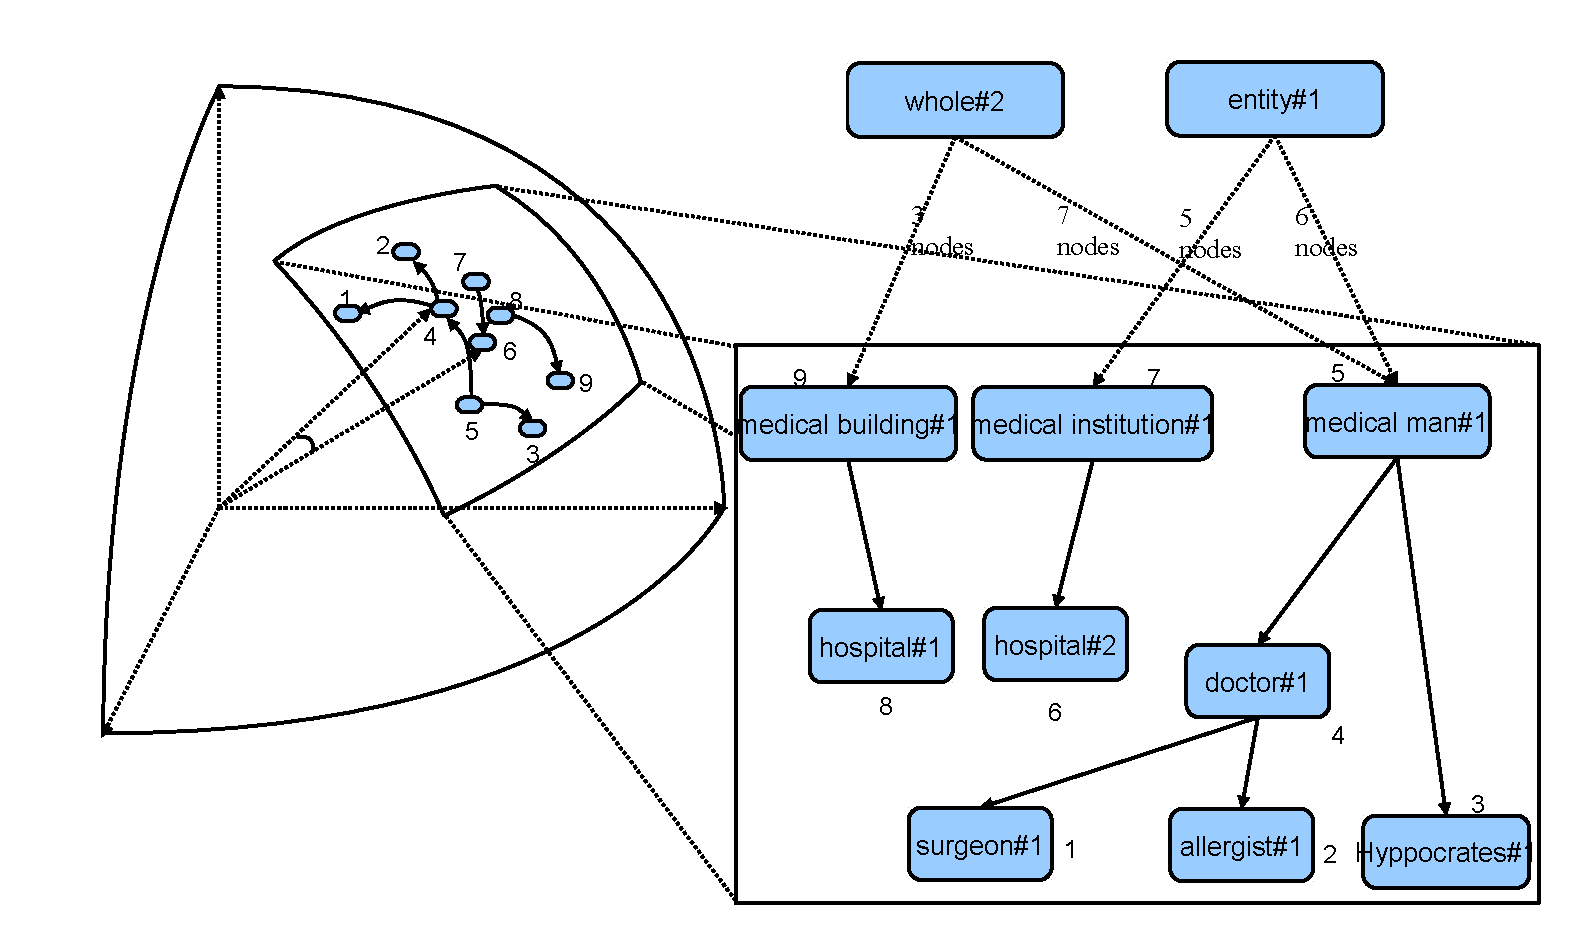
\includegraphics[width=15cm]{2_Etat-art/img/Projection-reseau}}
\caption{Projection d'un réseau (ici WordNet) sur une hyper-sphère de rayon 1}
\label{emergence-VC}
\end{figure}

En pratique, par construction, les composantes des vecteurs
d'idées\index{vecteurs! d'idées} sont positives. On peut donc dire que
ce sont des vecteurs de $\vrn$.  En toute généralité, et pour
respecter les axiomes des \index{espace vectoriel! normé} espaces
vectoriels normés, nous n'oublierons pas que les vecteurs
d'idées\index{vecteurs! d'idées} sont des vecteurs de $\R^n$.
Toutefois, par souci de simplification, lorsqu'il s'agira de définir
les opérations sur les vecteurs, nous prendrons en compte la
positivité des composantes des vecteurs, en particulier en ce qui
concerne les domaines de définition.

%Profitons de ce point pour essayer d'éviter une erreur parfois
%commise. L'espace des vecteurs d'idées\index{vecteurs! d'idées}
%associés à des segments textuels $\EnsVC$ est-il un sous-espace
%vectoriel de $\R$? Pour être un sous-espace vectoriel, il faut que
%$\EnsVC$ soit stable par \index{sous-espace vectoriel} combinaison
%linéaire (cf.  \ref{sec:sous-espac-vectoriel}) c'est-à-dire que nous
%devons avoir~:
%\\
%$$\forall u,v \in \EnsVC,\: \forall \alpha,\beta \in \R,\: \alpha
%u+\beta v \in \EnsVC $$
%\\
%Or cette propriété n'est pas vérifiée à cause de la normalisation des
%vecteurs. Ainsi, 
Précisons toutefois que l'espace des vecteurs d'idées n'est pas un
  sous-espace vectoriel dont les vecteurs génératifs seraient une base
  ou une famille génératrice.

\index{vecteurs! d'idées}
\index{sous-espace vectoriel}
\index{vecteurs génératifs}


Formellement, nous avons $\EnsVC \equiv \R^n$. Toutes les opérations
vectorielles qu'il est possible d'effectuer dans un espace vectoriel
normé \index{espace vectoriel! normé} sont
donc réalisables dans $\EnsVC$.  La différence est que nous cherchons
à donner à ces vecteurs une interprétation linguistique voire
psycholinguistique. Ils représentent des idées qui peuvent faire
référence éventuellement à un item lexical, un terme de la langue.
Les opérations réalisables sur les \index{vecteurs! d'idées} vecteurs
d'idées peuvent donc elles aussi avoir des interprétations
linguistiques qu'il convient d'analyser.  
%Nous nous appliquerons dans la suite de cette thèse à donner, autant que faire se peut, des
%interprétations linguistiques aux opérations présentées.

\paragraph{Vecteurs normés}

Dans notre modèle, la norme n'est pas considérée comme une information
qualitative. En effet, nous considérons que les idées ne prennent sens
que si elles sont appréciées les unes par rapport aux autres. Cette
affirmation est vraie tant à l'intérieur des vecteurs qu'entre les
vecteurs. Ainsi, il est plus pertinent de comparer les proportions des
différentes idées à l'intérieur d'un terme, d'un vecteur, plutôt que
de les analyser de façon absolue.

Il en est de même entre deux vecteurs. Que signifierait la comparaison
de deux vecteurs qui n'ont pas la même norme? Si on prend l'exemple du
calcul du vecteur d'idées\index{vecteurs! d'idées} d'un texte
quelconque par une méthode d'analyse sémantique (cf.
\ref{sec:remonte-redescente}), le principe est, en schématisant
beaucoup, de faire une somme pondérée des vecteurs. Si les vecteurs
n'étaient pas normés, la norme d'un vecteur serait un simple
indicateur de la longueur du texte à partir duquel il a été construit.

Si, au cours des opérations que nous présenterons par la suite
(cf.~\ref{operateurs}), la norme d'un vecteur n'est pas toujours égale
à l'unité, en particulier dans le cas de l'utilisation du produit
terme à terme, il n'en est jamais de même lorsqu'il s'agit d'un
vecteur correspondant à un segment textuel. Par exemple, les vecteurs
d'idées\index{vecteurs! d'idées} stockés dans une base de données
vectorielle ont tous une norme égale à 1.

\subsubsection{Distance et voisinage thématique}
\index{distance! thématique} \index{voisinage! thématique}

Un des premiers outils utilisés pour vérifier la cohérence d'une base
de vecteurs d'idées\index{vecteurs! d'idées} a été la fonction de
voisinage thématique. Elle permet de connaître les items dont le
vecteur est le plus proche du vecteur d'un item donné. Cette fonction
de voisinage est basée sur la notion de distance thématique.

\paragraph{Distance thématique} \label{sec:distance-thematique}
\index{distance! thématique}

Il est souvent souhaitable de pouvoir mesurer la proximité entre deux
items, c'est-à-dire une distance (ou au moins une mesure) entre leurs
vecteurs d'idées.\index{vecteurs! d'idées} Ces opérations peuvent
permettre non seulement d'estimer la cohérence d'une base de vecteurs
mais aussi s'avèrent souvent déterminantes pour connaître le sens d'un
terme. Il existe de nombreuses distances possibles entre vecteurs, la
thèse de \index{Besançon Romaric} Romaric Besançon
\cites{Besancon2001}{2.2.5} en fait une bonne synthèse. Dans le cadre
des \index{vecteurs! d'idées} vecteurs d'idées, la distance angulaire
est utilisée pour les opérations de base. En effet, elle permet une
meilleure discrimination pour les faibles angles et offre
d'intéressantes interprétations géométriques.

Par abus de langage nous parlerons
parfois de distance entre deux segments textuels au lieu de parler de
distance entre les vecteurs associés à ces deux segments.

\subparagraph{Similarité et distance angulaire}
\index{distance! thématique}

Soit $Sim(X,Y)$ une des mesures de \emph{similarité} entre deux
vecteurs X et Y, utilisée habituellement en recherche d'informations
\citep{SalMac1983}{121}.  Cette valeur est le cosinus de l'angle entre
les deux vecteurs.

\begin{equation}\label{formSimilarite}
\EnsVC^{2}\rightarrow [0,1]: \quad Sim(X,Y) = \cos(\widehat{X,Y})  =  {X \cdot Y \over\|X\|\times \|Y\|}\\
\end{equation}

Nous définissons la fonction de \emph{distance thématique} $D_{A}$
entre deux vecteurs $X$ et $Y$ comme la distance angulaire entre les
deux vecteurs.

\begin{equation}\label{formDistAng}
\EnsVC^{2}\rightarrow [0,\frac{\pi}{2}]: \quad D_{A}(X,Y) = \arccos(Sim(X,Y))
\end{equation}

Par définition, nous posons~:

\begin{equation}\label{eq:5}
D_{A}(\veczero,\veczero) = 0 \quad et \quad D_{A}(X,\veczero) = \frac{\pi}{2}
\mbox{ si }X \neq \veczero
\end{equation}
avec $\veczero$ dénotant le vecteur nul. Précisons que ce vecteur n'a
sans doute pas de représentation en langue. Il s'agirait d'un mot qui
n'active aucun concept, l'idée vide.

La distance angulaire est une vraie distance puisqu'elle vérifie les
propriétés de réflexivité, symétrie et inégalité triangulaire.
%
\begin{equation}
  s\acute{e}paration~: D_A(X, Y ) = 0 \Leftrightarrow X = Y \label{eq:1}
\end{equation}
\begin{equation}
  sym\acute{e}trie~: D_A(X, Y) = D_A(Y, X)\label{eq:2}
\end{equation}
\begin{equation}
  in\acute{e}galit\acute{e} \ triangulaire~: D_A(A,B)+D_A(B,C)\geq D_A(A,C)\label{eq:3}
\end{equation}
%

\subparagraph{Pourquoi choisir l'angle entre les deux vecteurs?}\label{sec:pourq-chois-langle}

Observons la figure \ref{arcos}. L'arc cosinus est une fonction
décroissante par rapport à la similarité. Plus cette dernière est
grande, plus l'angle entre les deux vecteurs est important. Cette
fonction est intéressante dans notre problématique car elle est
fortement non linéaire par rapport à la similarité pour les faibles
valeurs de l'angle (en dessous de $\frac{\pi}{4}$, là où les
comparaisons à effectuer sont les plus fines) tandis qu'elle est
pratiquement linéaire au-delà de $\frac{\pi}{4}$.

\begin{figure}[h]
  \centering{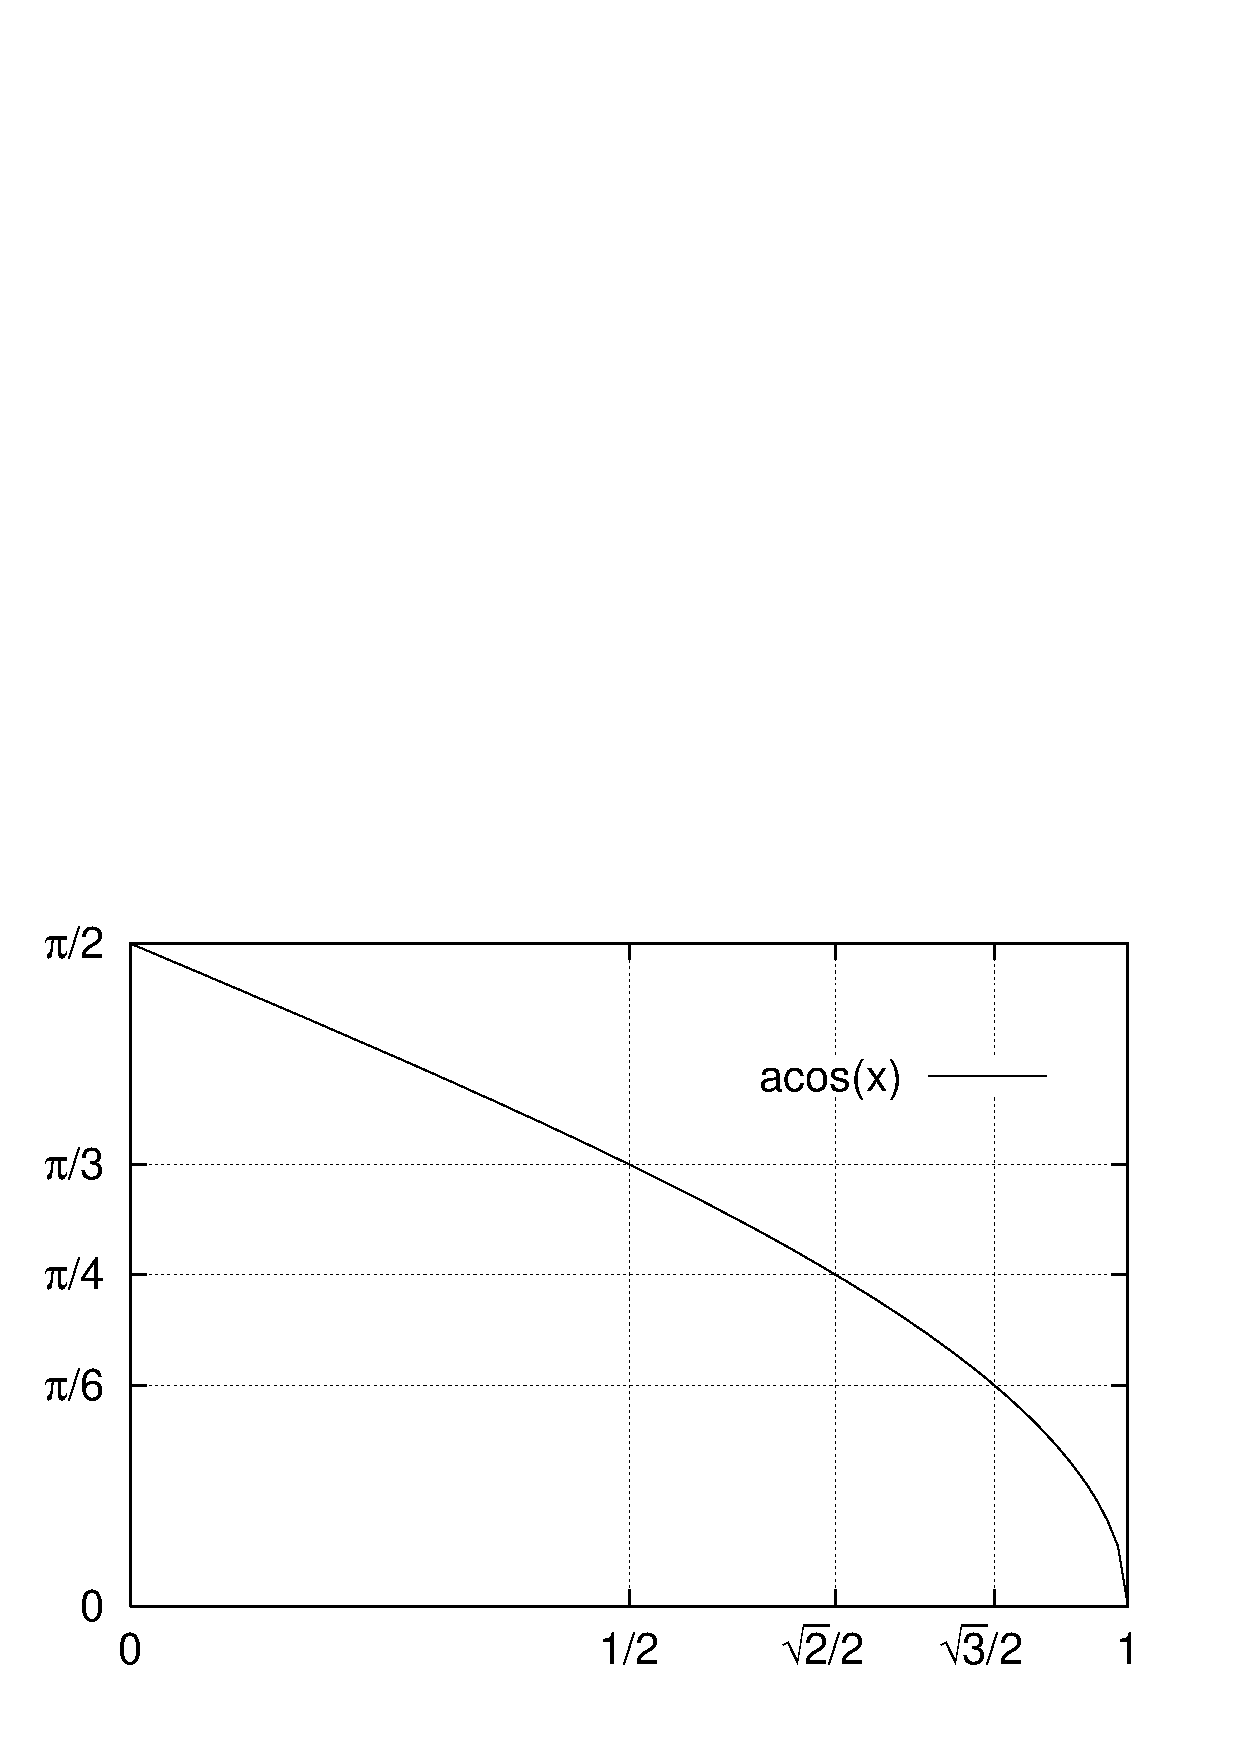
\includegraphics[width=10cm]{2_Etat-art/img/acos}}
\caption{fonction arc cosinus}

\label{arcos}
\end{figure}

En effet, un des objectifs des \index{vecteurs! d'idées} vecteurs
d'idées est de participer à des tâches de désambiguïsation sémantique.
Il peut arriver que les différences entre les sens soient relativement
faibles. Par exemple, l'éloignement des sens \annot{agneau}{viande} et
\annot{agneau}{animal} semble assez peu important. C'est une des
propriétés qui a entraîné le choix de l'angle entre les vecteurs comme
l'un de nos principaux outils. La deuxième 
concerne les relativement bonnes interprétations
géométriques qu'il est possible d'effectuer.

\subparagraph{Exemples}
\index{distance! thématique}

Le tableau \ref{fig:ex-dist-them} présente les distances thématiques
(en radians) entre les vecteurs de plusieurs termes. Ces exemples sont
réalisés à partir de la base de \index{vecteurs! conceptuels} vecteurs
conceptuels dont l'architecture est présentée en
\ref{sec:vectconcept}.

\begin{figure}[h]
  
  {\fontsize{8}{11}\selectfont
    \begin{tabular}{|c|c|c|c|c|c|c|c|c|c|c|}
      \hline
      \backslashbox{}{$D_A$}&destinée&destin&vie&existence&mort&automobile&train&action&inaction&réaction\\
      \hline
      destinée&0&0,51&0,82 &0,7 &0,99&1,29&1,38&1,31&1,14&1,2\\
      \hline
      destin&&0&0,83&0,75&0,99&1,3&1,38&1,25&1,07&1,16\\
      \hline
      vie&&&0&0,61 &0,89&1,28&1,35&1,3&1,1&1,2\\
      \hline
      existence&&&&0&0,98&1,37&1,43&1,37&1,25&1,3\\
      \hline
      mort&&&&&0&1,33&1,4&1,32&1,15&1,26\\
      \hline
      automobile&&&&&&0&0,88&1,4&1,22&1,29\\
      \hline
      train&&&&&&&0&1,43&1,3&1,39\\
      \hline
      action&&&&&&&&0&1,01&0,67\\
      \hline
      inaction&&&&&&&&&0&0,9\\
      \hline
      réaction&&&&&&&&&&0\\
      \hline
       \end{tabular}
      \caption{Exemples de résultats de la distance thématique \dang{X}{Y}.}
      \label{fig:ex-dist-them}
    }
    \end{figure}
    \index{vecteurs! d'idées}
    
    Le tableau est symétrique (symétrie de \dang{X}{Y}) et la
    diagonale est toujours égale à 0 (réflexivité de \dang{X}{Y}). On
    remarquera qu'une valeur prend toute sa signification relativement
    à une autre. En particulier, il est satisfaisant d'avoir~:

\begin{itemize}
\item \dang{\lexItem{destin}}{\lexItem{destinée}} $\leq$
  \dang{\lexItem{destinée}}{\lexItem{vie}} et
  \dang{\lexItem{existence}}{\lexItem{vie}} $\leq$
  \dang{\lexItem{destinée}}{\lexItem{vie}} ce qui correspond bien au
  fait que \lexItem{destin} et \lexItem{destinée} d'une part, et
  \lexItem{existence} et \lexItem{vie} sont plus proches que
  \lexItem{destinée} et \lexItem{vie}.
  
\item \dang{\lexItem{vie}}{\lexItem{mort}} $> \frac{\pi}{4}$ (0,78) ce
  qui dénote un certain éloignement des idées.
  
\item\dang{\lexItem{vie}}{\lexItem{automobile}} $> \frac{\pi}{3}$
  (1,04) ce qui relève d'un éloignement important.
  
\item \dang{\lexItem{action}}{\lexItem{réaction}} est la plus petite
  valeur de \dang{\lexItem{action}}{Y} car les deux concepts
  \cname{action} et \cname{réaction} sont relativement proches et que
  \lexItem{action} partage beaucoup moins d'idées avec les autres
  termes.
\end{itemize}

\subparagraph{Interprétations}
\index{distance! thématique} \index{vecteurs! d'idées}

On remarquera qu'habituellement, les comparaisons entre les valeurs
sont plus significatives que les valeurs elles-mêmes, toutefois, on
estime empiriquement que~:
\begin{itemize}
\item si $D_{A}(X,Y) \leq \frac{\pi}{4}$, $X$ et $Y$ partagent des
  concepts et sont considérés comme sémantiquement proche.
\item si $D_{A}(X,Y) \geq \frac{\pi}{4}$, la proximité sémantique de
  $A$ et $B$ est considérée comme faible.
\item Aux alentours de $\frac{\pi}{2}$, les sens sont sans rapport.
\end{itemize}

Intuitivement, cette fonction constitue une évaluation possible de la
\emph{proximité thématique}.  La métaphore de la nuit étoilée peut
aider à appréhender cette idée de distance angulaire pour calculer la
proximité thématique. Nous pouvons nous représenter l'espace des sens
comme un ciel rempli d'étoiles. Les étoiles sont les items lexicaux.
Les mots, tout comme les étoiles, forment des constellations.
Certaines parties de l'espace sont très densément peuplées tandis que
d'autres sont quasi-désertes. Un sens est une direction de l'espace et
non un point. Un observateur ne peut connaître exactement la distance
entre une étoile et lui-même mais il connaît la direction de l'astre.
Dans le ciel, la distance entre deux étoiles est la distance
apparente, l'angle entre les deux. Il en est de même, dans notre
espace, avec les items lexicaux.\index{distance! thématique}

\paragraph{Voisinage thématique}\label{sec:voisinage}
\index{vecteurs! d'idées} \index{voisinage! thématique}

La fonction de voisinage thématique permet de connaître les items
lexicaux voisins d'un item lexical donné.  On définit $\vois$ la
fonction de proximité thématique qui renvoie les $k$ items les plus
proches en termes de distance angulaire d'un texte $Z$ dans une base
vectorielle. Soit~:

\index{distance! thématique}

\begin{equation}
  \label{eq:voisinage}
  \left|{\cal V}(Z)\right|= k \qquad
  \forall X \in {\cal V}(Z), \quad  \forall Y \notin {\cal 
    V}(Z), \quad  \mbox{\dang{X}{Y}} \leq \mbox{\dang{Y}{Z}}
\end{equation}

Par exemple, les termes proches et ordonnés par distance thématique
\index{distance! thématique} croissante des mots \lexItem{vie},
\lexItem{ranger} et \lexItem{couper} pourraient être~:

$\cal V($\lexItem{vie}) = \lexItem{vie quotidienne}, \cname{vie},
\lexItem{s'animer}, \lexItem{demi-vie}, \lexItem{survivant},
\lexItem{avoir la vie devant soi}, \lexItem{naissance},
\lexItem{viabilité}, \lexItem{vital}, \lexItem{naître},
\lexItem{vivant}, \lexItem{assurance-vie},\ldots
  
$\cal V($\lexItem{ranger}) = \lexItem{trier}, \lexItem{cataloguer},
\lexItem{sélectionner}, \lexItem{classer}, \lexItem{distribuer},
\lexItem{grouper}, \lexItem{ordonner}, \lexItem{répartir},
\lexItem{aligner}, \lexItem{caser}, \lexItem{arranger},
\lexItem{nettoyer}, \lexItem{distribuer}, \lexItem{démêler},
\lexItem{ajuster}, \ldots

$\cal V($\lexItem{couper}) = \lexItem{cisailler}, \lexItem{émincer},
\lexItem{scier}, \lexItem{tronçonner} , \lexItem{ébarber},
\lexItem{entrecouper}, \lexItem{baptiser}, \lexItem{recouper},
\lexItem{sectionner}, \lexItem{bêcher}, \lexItem{hongrer},
\lexItem{essoriller}, \lexItem{rogner}, \lexItem{égorger},
\lexItem{écimer}, \ldots

\subsubsection{Opérations classiques}\label{operateurs}
\index{vecteurs! d'idées} Nous présentons ici les opérations
définies pour les vecteurs d'idées\index{vecteurs! d'idées} que nous
utilisons dans ce document.

\paragraph{Somme vectorielle}\label{sec:somme-vectorielle}

\subparagraph{Définition}
Soient $X$ et $Y$ deux vecteurs, leur \emph{somme vectorielle} V est
définie par~:

\begin{equation}
\EnsVC^{2} \rightarrow \EnsVC~: V = X + Y \quad \mid \quad V_{i} = X_{i} + Y_{i}
\end{equation}

où $V_i$ (resp $X_i$, $Y_i$) représente la i-ème composante du
vecteur V (resp. X, Y).
\\

Soient $X$ et $Y$ deux vecteurs, leur \emph{somme vectorielle normée}
V est définie par~:

\begin{equation}
\EnsVC^{2} \rightarrow \EnsVC~: V = X \vecadd Y \quad \mid \quad V_{i} = \frac{X_{i} + Y_{i}}{\|X+Y\|}
\end{equation}

L'opérateur $\vecadd$ est idempotent et nous avons $X\vecadd X = X$.
Le vecteur nul $\veczero$ est l'élément neutre de la somme vectorielle
et, par définition, on pose,
\begin{equation}
\veczero \vecadd \veczero = \veczero.
\end{equation}

\begin{figure}[h]
  \centering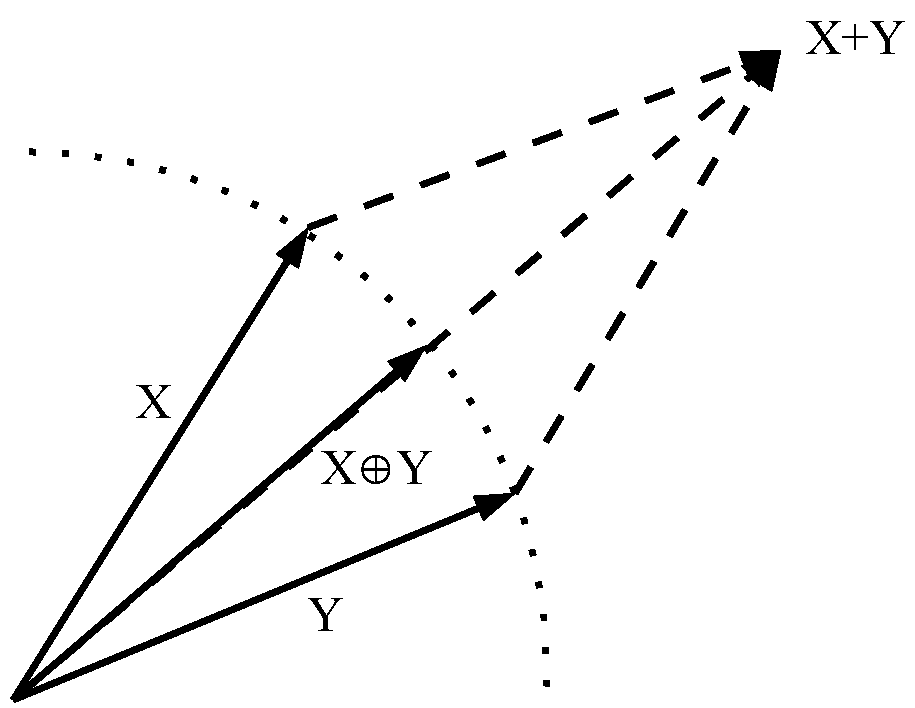
\includegraphics[width=8cm]{2_Etat-art/img/exempleSommeNormee}
\caption{Somme vectorielle normée} 

\label{schema_general}
\end{figure}

De ce qui précède, on peut facilement déduire les propriétés de
rapprochement (local et généralisé)~:
\begin{equation}
D_{A}(X\vecadd X,Y\vecadd X) = D_{A}(X,Y \vecadd X) \leq D_{A}(X,Y)
\end{equation}
\begin{equation}
D_{A}(X\vecadd Z,Y\vecadd Z) \leq D_{A}(X,Y)
\end{equation}

La somme vectorielle est généralisée à n'importe quel nombre de
vecteurs par~:

\begin{equation}
\EnsVC^{n} \rightarrow \EnsVC~: V =\sum^{n}_{i=1} V(x_i) \quad \mid
\quad V_j = \sum_{j=1}^{n} V(x_i)_j
\end{equation}

où $V(x_i)$ représente le vecteur d'idée de l'objet $x_i$, $V_j$ et
$V(x_i)_j$ la j-ème composante des vecteurs $V$ et $V(x_i)$. La somme
vectorielle normée est généralisée à n'importe quel nombre de vecteurs
par~:

\begin{equation}
\EnsVC^{n} \rightarrow \EnsVC~: V=\bigvecadd^{n}_{i=1} V(x_i) \quad \mid \quad V_j=\frac{\sum_{j=1}^{n} V(x_i)_j}{\|\sum^{n}_{i=1} V(x_i)\|}
\end{equation}

%\subparagraph*{Précision importante sur la notation}

Précisons que la somme vectorielle normée binaire n'est pas associative. Toutefois,
pour pouvoir simplifier, nous écrirons
%
$\bigvecadd^{n}_{i=1} V(x_i)$ au lieu de $ V(x_1) \vecadd V(x_2)
\vecadd \ldots \vecadd V(x_n)$.

\subparagraph{Interprétation}\index{vecteurs! d'idées}

La somme vectorielle normée de deux vecteurs donne un vecteur
équidistant en termes d'angle des deux premiers vecteurs. Il s'agit en
fait d'une moyenne des vecteurs sommés. En tant qu'opération sur les
vecteurs d'idées,\index{vecteurs! d'idées} on peut donc voir la somme
vectorielle normée comme l'union des idées contenues dans les termes.

\paragraph{Produit terme à terme}\label{sec:produit-terme-terme}

\subparagraph{Définition}
Soient $X$ et $Y$ deux vecteurs, leur \emph{produit terme à terme} $V$
est défini par~:
\begin{equation}
\EnsVC^{2} \rightarrow \EnsVC~: V = X \vecptt Y \quad  \mid \quad  v_{i} = x_iy_i
\end{equation}

Soient $X$ et $Y$ deux vecteurs, leur \emph{produit terme à terme
  normalisé} $V$ est défini par~:
\begin{equation}
\EnsVC^{2} \rightarrow \EnsVC~: V = X \vecpttnorm Y \quad  \mid \quad  v_{i} = \sqrt{x_iy_i}
\end{equation}

Cet opérateur est idempotent (${X \vecpttnorm X = X}$) et $\veczero$
est absorbant (${X \vecpttnorm \veczero = \veczero}$).  Il peut être
généralisé à n'importe quel nombre de vecteurs par:
\begin{equation}
\EnsVC^{n} \rightarrow \EnsVC~: V = \bigotimes^{n}_{i=1} V(x_i) \quad  \mid \quad V_j = \sqrt[n]{\prod_{j=1}^{n}V(x_i)_j}
\end{equation}

L'opérateur $\otimes$ peut être interprété comme un opérateur
d'intersection entre vecteurs. Si l'intersection entre deux vecteurs
est le vecteur nul, alors ils n'ont rien en commun. On a, de plus, la
propriété suivante~:

\begin{equation}
\forall X \neq \veczero \quad \forall Y \neq \veczero \quad X \otimes
Y = \veczero \Leftrightarrow D_A(X,Y)=\frac{\pi}{2}
\end{equation}

\subparagraph{Interprétation}

Comme nous venons de le dire, l'opérateur $\otimes$ peut être vu comme
une intersection des vecteurs. Du point de vue des vecteurs
d'idées,\index{vecteurs! d'idées} cette opération permet donc de
sélectionner les idées communes à un ensemble de termes. Il est
utilisé en particulier dans l'opération de contextualisation faible.

\paragraph{Contextualisation faible} \label{sec:cont-faible}

Lorsque que deux termes sont en présence, pour chacun d'eux, certaines
idées se trouvent sélectionnées par le contexte que constitue l'autre
terme. Ce phénomène de \emph{contextualisation} consiste à augmenter
chaque vecteur de ce qu'il a de commun avec l'autre. Comme nous venons
de le voir, les idées communes à deux termes sont données par le
produit terme à terme. Ainsi, nous pouvons définir la
contextualisation faible $\con(X,Y)$ des vecteurs $X$ par $Y$ par:

\begin{equation}
\EnsVC^{2} \rightarrow \EnsVC~: \con(X,Y) = X \vecadd (X \vecptt Y)
\end{equation}

Cette fonction n'est pas symétrique. L'opérateur $\con$ est idempotent
($\con(X,X) = X$) et le vecteur nul est un élément neutre
($\con(X,\veczero) = X \vecadd \veczero = X$).

La propriété de \emph{rapprochement} suivante peut être tirée~:

\begin{equation}
D_{A}(\con{(X,Y)},\con{(Y,X)}) \leq D_{A}(\con{(X,Y)},Y) \leq D_{A}(X,Y)
\end{equation}
%
\begin{equation}
D_{A}(\con{(X,Y)},\con{(Y,X)}) \leq D_{A}(X,\con{(Y,X)}) \leq D_{A}(X,Y)
\end{equation}

La contextualisation $\con{(X,Y)}$ rapproche les vecteurs $X$ de $Y$
proportionnellement à leur intersection.

%\subsubsection{Statistiques}

%Le but de cette section est de rappeler quelques formules de
%statistiques que nous pouvons appliquer sur les composantes $V_i$ d'un vecteur d'idée quelconque $V$.  Nous présentons autant que possible
%les interprétations que nous pouvons faire de l'application de ces formules sur des vecteurs~:

%\paragraph{Moyenne}

%La moyenne arithmétique $\mu$ de N valeurs est:

%\begin{equation}
%\mu=\frac{\sum_{i=1}^{N}x_i}{N}
%\end{equation}

%\paragraph{Variance}

%La variance $v$ est donnée par la formule:
%\begin{equation}
%v=\frac{\sum_{i=1}^{N}(x_i-\mu)^2}{N}
%\end{equation}

%\paragraph{\'Ecart type}

%L'écart type $e$ est défini par:
%\begin{equation}
%e=\sqrt{v}
%\end{equation}

%\paragraph{Coefficient de variation} \label{sec:coeff-de-variation}

%Le coefficient de variation $c$ est donné par:

%\begin{equation}
%c = \frac{e}{\mu}
%\end{equation}

%Le coefficient de variation n'est défini que lorsque $\mu \neq 0$.
%Toutefois, il peut être arbitrairement étendu pour tenir compte du
%vecteur nul~:

%\begin{equation}
%c(\vec{0})=0
%\end{equation}

%Dans le cadre des vecteurs d'idées,\index{vecteurs! d'idées} on peut
%voir le coefficient de variation $c$ comme une mesure statistique
%normalisée (sans unité) de la "conceptualité" du vecteur $V$.  Il est
%d'autant plus important que les composantes du vecteur sont
%contrastées et vaut 0 si elles ont toutes la même valeur $\frac{\sqrt
  %n}{n}$.

\subsubsection{Analyse sémantique de textes~: l'algorithme de
  remontée-redescente}\label{sec:remonte-redescente}

\index{analyse sémantique! par remontée-redescente}

%% MOT ici sur l'analyse syntaxique utilisée dans nos expériences : détailler sygfran ?
%% actualiser : campagne easy finie, passage à la suite

%\paragraph{Niveau syntaxique dans le cadre de cette thèse :
 % SYGFRAN}\label{sec:SYGFRAN}

%Les membres de l'équipe TALN\index{TALN} du LIRMM utilisent dans leurs
%expérimentations sur le français l'analyseur morpho-syntaxi\-que
%SYGFRAN.  Il s'agit d'un programme développé grâce à SYGMART (SYstème
%Grammatical de Manipulation Algorithmique et Récursive de Texte), un
%outil qui permet de construire des applications traitant des notions
%de morphologie, de syntaxe et/ou de sémantique \cite{Chauche1984}.
%SYGMART est un système transformationnel d'arborescences fondé sur les
%algorithmes de Markov étendus aux arbres. Il permet d'analyser tout
%langage dont la grammaire pourrait être écrite sous forme de
%transducteurs d'arbres.  L'application pour le français, SYGFRAN
%comporte environ 11000 règles\footnote{En Janvier 2005.} inspirées des
%travaux du linguiste Jürgen Weissenborn. SYGMART et son application
%SYGFRAN sont développées par Jacques
%Chauché\footnote{\url{http://www.lirmm.fr/~chauche/Pr\%E9sentationSygmart.html}}.
%SYGFRAN renvoie, pour un texte quelconque en français, l'arbre
%morpho-syntaxique correspondant. Un exemple d'analyse rendue par
%SYGFRAN est celui de la phrase \sentence{Le petit chat boit du lait.}
%présenté dans la figure \ref{fig:chatboit-lait-analyse-synt}.

%L'utilisation de SYGFRAN offre deux principaux avantages :

%\begin{itemize}
  
%\item \emph{Analyse robuste} : SYGFRAN propose une analyse robuste. En
 % effet, même lorsque certains termes sont inconnus, même si la phrase
 % est agrammaticale, il en propose une analyse partielle et indique
 % ses incertitudes ;
  
%\item \emph{Rapidité} : Un deuxième grand avantage de SYGFRAN est sa
  %rapidité. En effet, sa complexité théorique est relativement faible
  %: $O(m \times n \times log_2(n))$ où $n$ est la taille de la donnée
  %et $m$ le nombre de règles. En pratique, les résultats sont aussi
  %très intéressants.  L'analyseur vient de participer à la campagne
 % EASY (\'Evaluation des Analyseurs Syntaxiques du Français).  Si nous
 % n'avons pas, à l'heure où nous écrivons ces lignes, les résultats,
  %nous pouvons présenter les temps qu'il a fallu pour annoter le
 % corpus d'évaluation de l'ELDA (Evaluation and Language Resources
 % Distribution Agency) utilisé pour la campagne.
%\begin{figure}[H]

  %\begin{center}

 %\begin{tabular}{|c|c|c|c|}
    %  \hline
 %Corpus&taille&temps&vitesse\\
    %  \hline
      %\emph{Le Monde}&471 Ko&42 min&11.2 Ko.min$^{-1}$\\
      %\hline
      %\emph{littéraire}&439 Ko&48 min& 9.1 Ko.min$^{-1}$\\
      %\hline
      %\emph{médical}&119 Ko&9 min&13.2 Ko.min$^{-1}$\\
      %\hline
      %\emph{global}&4.19 Go&7H13& 9.67 Ko.min$^{-1}$\\
      %\hline
    %\end{tabular}

 %\caption{Extrait des temps réalisés par SYGFRAN pour effectuer
  % l'analyse syntaxique des textes du corpus de l'ELDA avec un Pentium
   %IV 2,4Ghz (4734 Bigomips) 1Go Ram}

  %\end{center}
%\end{figure}

%Comme nous pouvons le constater, SYGFRAN est très rapide. Sa vitesse
%d'analyse varie, suivant le type de corpus, entre $9.1Ko.min^{-1}$
%pour un corpus littéraire et $13.2 Ko.min^{-1}$ pour un corpus
%médical. Cette différence s'explique par la longueur des phrases
%nettement plus importante pour le corpus littéraire. Quoi qu'il en
%soit, pour des textes de longueur moyenne, la durée d'une analyse est
%de l'ordre de 10 secondes.
%\end{itemize}

L'objectif des vecteurs d'idées est d'améliorer la plupart des
applications du TALN où la sémantique peut jouer un rôle. %Citons quelques exemples. 
En \emph{recherche documentaire}, on peut dans une
phase de préparation des données affecter un vecteur à chaque texte et
dans une phase d'exploitation renvoyer les plus proches du vecteur
d'une requête; en \emph{traduction automatique} il peut s'agir de
trouver le vecteur correspondant à l'équivalent le plus proche dans
une langue cible; en
\emph{résumé automatique de textes} on peut choisir de privilégier une
partie du texte qui représente mieux les idées principales du discours
général plutôt qu'une autre; en \emph{catégorisation} on peut
regrouper les textes les plus proches suivant une méthode basée sur la
distance angulaire, \ldots} L'idée sous-jacente est donc de pouvoir
affecter un vecteur d'idées\index{vecteurs! d'idées} à tout segment
textuel et c'est dans cette perspective qu'a été définie l'analyse
sémantique de textes.  Cette analyse est différente suivant le type de
vecteurs utilisés (sémantique\footnote{non développée dans ce document.} ou conceptuel) cependant le principe
général est le même.

\paragraph{Principe}
\label{sec:principe-analyse-sem}

L'analyse sémantique de textes permet de calculer le vecteur d'idées
d'un texte quelconque. Son principe général est de se baser sur
l'hypothèse de compositionnalité de la sémantique linguistique
c'est-à-dire que \sentence{le tout est calculable à partir du sens de
  ses parties} (cf. \ref{sec:semantique}). Le vecteur d'un texte est
donc calculé de façon générale par une fonction ayant pour paramètres
l'ensemble des vecteurs d'idées\index{vecteurs! d'idées} des items du
texte.  En pratique, il s'agit d'une somme pondérée des vecteurs
contextualisés des termes de ce texte.

L'idée originale de cette opération est de se baser sur une analyse
morpho-syntaxique préliminaire telle que celle présentée en
\ref{sec:niveau-syntaxique}. En effet, il a été montré que l'apport
d'informations syntaxiques pour la construction de vecteurs de type
saltonien donne de meilleures performances, entre autres, dans le
domaine de la recherche d'informations \cite{Besancon2001}. Ce constat
peut être renouvelé avec les \index{vecteurs! d'idées} vecteurs
d'idées. L'analyse morpho-syntaxique réalisée permet de pondérer par
un scalaire le vecteur de chaque mot ou groupe de mots en fonction de
son rôle syntaxique \cite{Chauche2003}. Ainsi, dans le segment
\sentence{voile de bateau}, \lexItem{voile} est gouverneur syntaxique,
son vecteur aura donc un poids plus important que \lexItem{bateau}. En
revanche, l'inverse sera appliqué pour \lexItem{bateau à voile}.

La méthode utilisée se différencie sur la
manière d'utiliser le contexte ainsi que sur l'affectation des
vecteurs aux feuilles.


\paragraph{Préformatage de textes}
\label{sec:preform-textes}

L'analyse sémantique des textes s'effectue donc en deux parties.  Dans
une première, on extrait la structure morpho-syntaxique que l'on
utilise dans une deuxième partie pour calculer un vecteur
d'idées.\index{vecteurs! d'idées} Il est clair que la première partie
influence grandement la seconde. En effet, une mauvaise analyse
morpho-syntaxique peut faire insister l'analyse sémantique sur des
aspects du texte moins pertinents, par exemple si un gouverneur est
mal identifié, voire erroné si l'arbre indique des morphologies ou des
fonctions syntaxiques incorrectes. Ce type d'erreur est généré lorsque
l'analyseur syntaxique est confronté à des termes qui lui sont
inconnus. Un préformatage à partir des informations contenues dans la
base de données vectorielle peut influencer bénéfiquement l'analyseur
morpho-syntaxique en lui indiquant quelles morphologies sont possibles
pour tel ou tel terme.  Cette étape préliminaire peut aussi permettre
de faciliter l'analyse sémantique si les textes contiennent des
constructions de phrases particulières ou de préparer les textes en
fonction d'une tâche spécifique. Le préformatage des textes vise donc
à améliorer soit l'analyse morpho-syntaxique soit la partie analyse
sémantique proprement dite.

\subparagraph{Préformatage pour améliorer l'analyse
  morpho-syntaxique}

Deux principaux préformatages peuvent être effectués pour améliorer
l'analyse morpho-syntaxique des textes~: la \emph{gestion des mots
  inconnus} et la \emph{reconnaissance des locutions}.

\begin{itemize}

\item \textit{Gestion des mots inconnus} Les mots inconnus pour
l'analyseur morpho-syntaxique entraînent souvent des erreurs dans
l'arbre renvoyé~: les constituants ne sont pas ou sont mal identifiés.
Ce genre de problème est extrêmement fréquent. Bien qu'il ne soit pas
rare de trouver des fautes d'orthographe quelle que soit la provenance
des textes (extraits de journaux, dictionnaires, dépêches d'agences,
etc.), la plupart des mots inconnus sont plutôt le fait de néologismes
ou de noms propres que l'analyseur ne peut pas forcément posséder. %Les
%fautes doivent être corrigées ou les informations complétées afin que
%l'analyse syntaxique soit la plus fiable possible. 
Des méthodes automatiques de correction existent. 
%En pratique, le texte est envoyé
%à l'analyseur syntaxique qui attire l'attention sur certains mots
%qu'il n'a pas réussi à identifier. Des systèmes experts capables de
%trouver dans la base de données vectorielle quels sont les termes les
%plus proches en fonction des informations présentes permettent alors
%de proposer une correction en cas de fautes d'orthographe ou indiquent
%quelles informations morphologiques utiliser. Le texte est alors
%annoté par des balises spécifiques et resoumis à l'analyseur
%morpho-syntaxique.  Par exemple, si nous prenons la phrase
%\sentence{Napoléon a été sacré en 1804.}, si Napoléon n'est pas
%reconnu au cours de l'analyse morpho-syntaxique, la phrase est
%resoumise balisée \sentence{@nom\_propre\_masculin\_singulier@Napoléon
 % a été sacré en 1804.}. L'analyseur peut alors renvoyer un arbre
%correct. Notons que soumettre à nouveau la requête à SYGFRAN n'est pas
%un réel problème puisque le temps de calcul de l'arbre d'une
%définition standard est négligeable (souvent très inférieur à la
%seconde) par rapport à l'analyse sémantique globale
%(cf.~\ref{sec:SYGFRAN}).

  
\item \textit{Reconnaissance des locutions} Un autre moyen d'aider
l'analyseur morpho-syntaxique est de lui indiquer les \emph{locutions
  semi-figées connexes}, c'est-à-dire les items dont la sémantique ne
peut pas être calculée uniquement à partir de la somme de leurs
parties.  C'est le cas par exemple de termes comme \lexItem{moulin à
  vent}, \lexItem{avion de chasse} ou \lexItem{lampe de chevet}. Il
est nécessaire de les indiquer à l'analyseur morpho-syntaxique afin
que celui-ci ne renvoie pas un sous-arbre pour ces mots.

\end{itemize}

\subparagraph{Préformatage pour améliorer l'analyse sémantique}

Le préformatage permet aussi de préparer le texte en vue de l'analyse
sémantique proprement dite. Il s'agit alors de préparer les textes en
vue d'une analyse spécifique comme c'est le cas avec le métalangage
des définitions pour les vecteurs conceptuels
(cf.~\ref{sec:formatage-defs}).\index{vecteurs! conceptuels}

%\section{Les vecteurs sémantiques}
%\label{sec:vect-semantiques}

%Les vecteurs sémantiques\index{vecteurs! sémantiques} sont le prolongement direct des travaux de \index{Chauché Jacques} Jacques
%Chauché initiés au début des années 1990 (cf.  \ref{sec:chauche}).  Il s'agit d'une formalisation de la projection de la notion linguistique
%de champ sémantique \index{champ sémantique} dans un espace vectoriel. \index{espace vectoriel} Après la traduction automatique, une des
%premières idées d'application est alors d'améliorer les analyses syntaxiques réalisées par SYGFRAN grâce à des informations de nature
%sémantique.  Par la suite, les applications sont devenues encore plus variées (catégorisation, résumé de textes).  Les vecteurs génératifs
%de l'espace des vecteurs sémantiques sont constitués à partir de la hiérarchie issue de \cite{Thesaurus1992}
%(cf.~\ref{sec:thes-hierarchie}). La version électronique de la troisième partie du thésaurus (cf.  \ref{sec:thes-index}) de ce
%thésaurus a permis d'indexer un ensemble important de termes généraux de la langue (environ 50000).

%\index{vecteurs génératifs! de l'espace des vecteurs! sémantiques}

%\subsection{Objectifs visés}

%Une des premières applications des vecteurs
%sémantiques\index{vecteurs! sémantiques} est d'améliorer les analyses
%syntaxiques réalisées par SYGFRAN. Il s'agit de pouvoir lever un
%certain nombre d'ambiguïtés relevées par l'analyseur. Par exemple, la
%phrase classique \sentence{La petite brise la glace} peut
%syntaxiquement avoir deux interprétations. Dans la première,
%\lexItem{petite} et \lexItem{glace} sont des noms, \emph{brise} est la
%troisième personne du présent de l'indicatif du verbe \lexItem{briser}
%tandis que dans la deuxième, \emph{petite} correspond à l'adjectif
%\lexItem{petit}, \emph{glace} au verbe \lexItem{glacer} et
%\lexItem{brise} est un nom (cf. figure \ref{fig:an-petite-brise}). Si
%syntaxiquement, il est absolument impossible de lever l'ambiguïté, des
%informations de nature sémantique sur le contexte de cette phrase
%peuvent permettre d'émettre des préférences.

%\begin{figure}[h]

  %\centering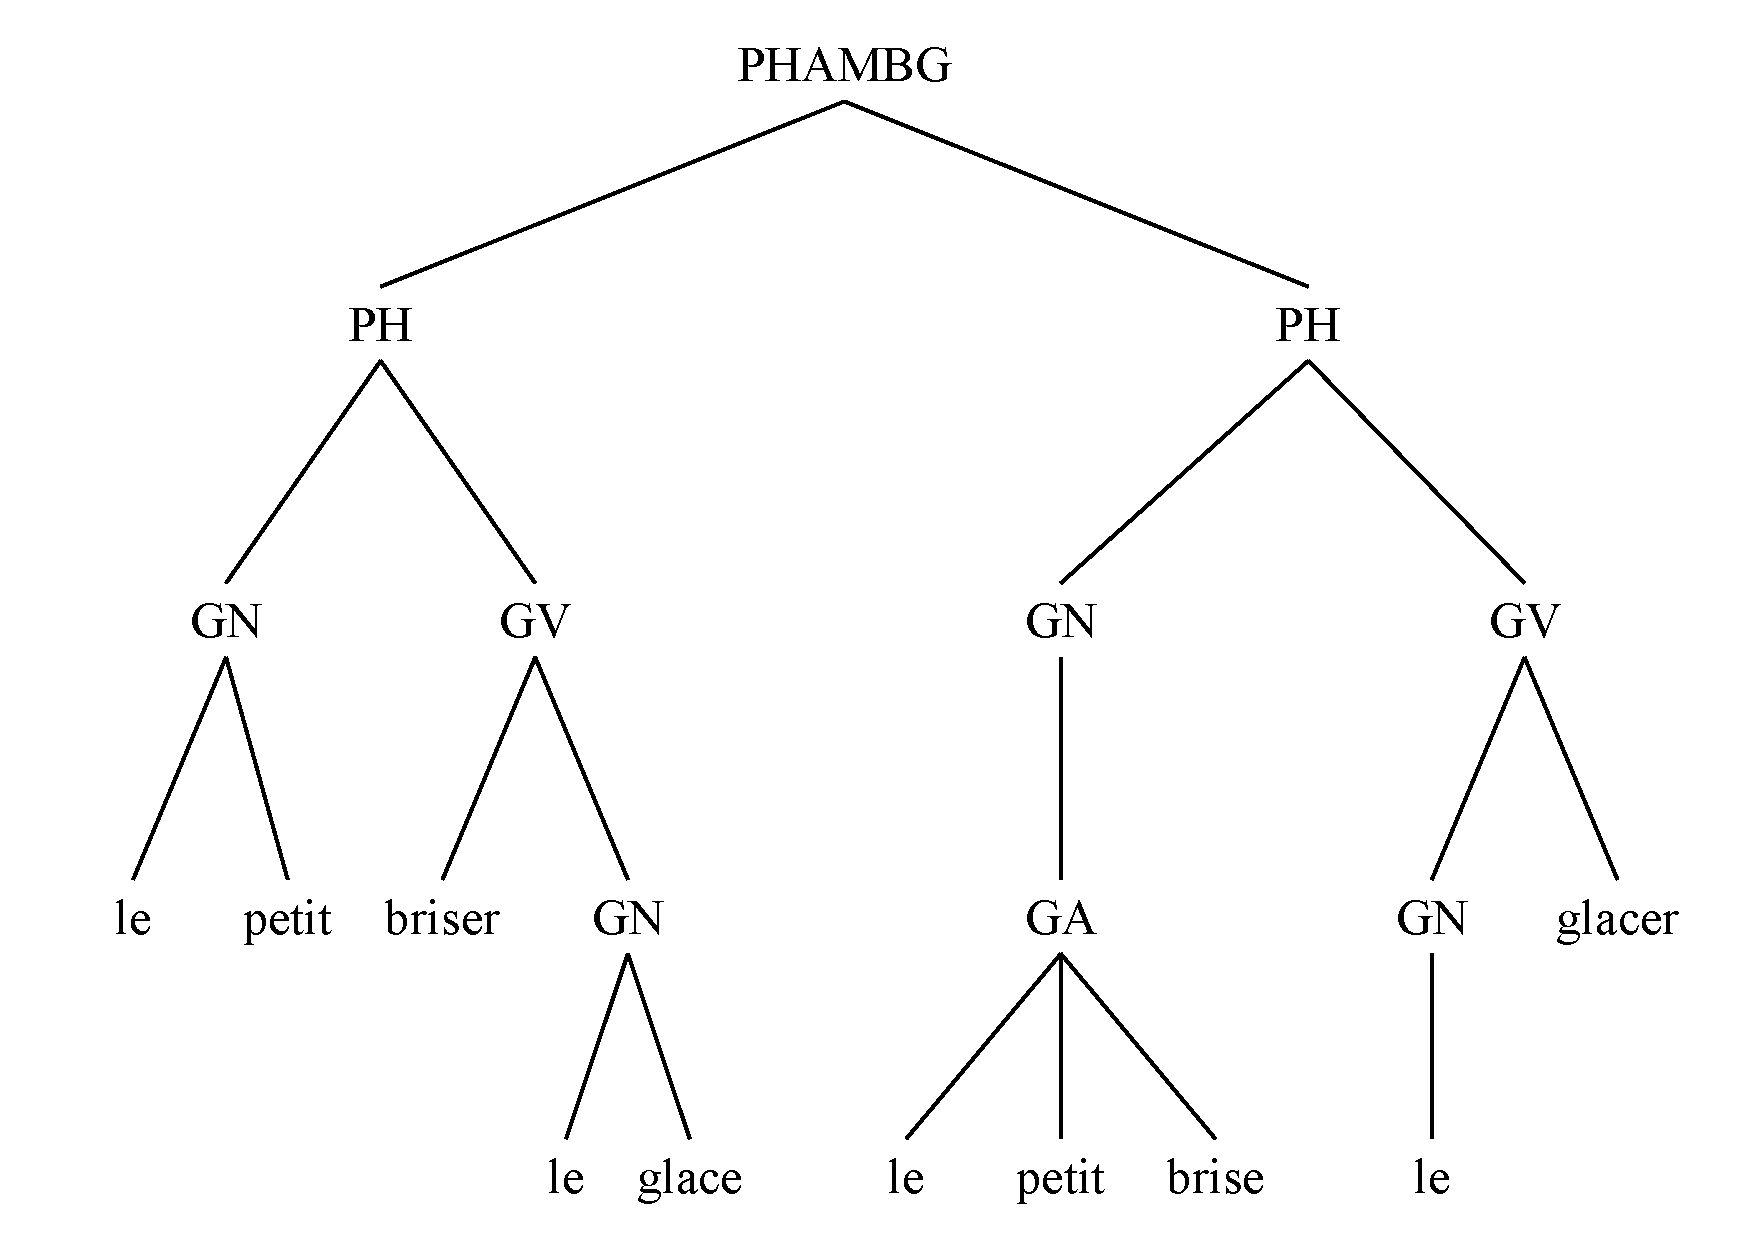
\includegraphics[width=10cm]{2_Etat-art/img/petite-brise-analyse-synt}
%\caption{Analyse syntaxique de la phrase \sentence{La petite brise la glace.}.}
%\label{fig:an-petite-brise}
%\end{figure}

%Les travaux ont été poursuivis par des essais sur la traduction du
%français vers le Tahitien (Eugène Sandford, Jacques
%Chauché)\index{Chauché Jacques} \cite{sandford1998} et sont
%actuellement menés par l'équipe sur la traduction du français vers
%l'anglais\footnote{\url{http://www.lirmm.fr/~prince/ExempleAnlTal.html}}
%(Violaine Prince), la catégorisation (Simon Jaillet, Jacques Chauché,
%Violaine Prince) \cite{Chauche2003} \cite{jaillet2005} ainsi que sur
%le résumé automatique (Mehdi Yousfi-Monod, Violaine Prince)
%\index{Prince Violaine} \index{Jaillet Simon} \cite{Yousfi-Monod2005a}
%\cite{Yousfi-Monod2005b} \index{Yousfi-Monod Mehdi}.

%\subsection{Architecture de la base}

%La fabrication des vecteurs sémantiques\index{vecteurs! sémantiques} a
%évolué au cours des années.  D'une utilisation de la partie
%\emph{organum} de l'encyclopédie Universalis (cf.~\ref{sec:chauche}),
%on est passé à l'usage du thésaurus Larousse, outil présenté comme
%permettant de couvrir l'ensemble des idées de la langue (hypothèse du
%thésaurus cf.  \ref{sec:thes-hierarchie}).

%\subsubsection{Vecteurs génératifs}\label{sec:vecteurs-generatifs}

%\index{vecteurs génératifs! de l'espace des vecteurs! sémantiques} Les
%vecteurs génératifs des vecteurs sémantiques sont fabriqués à partir
%de la partie index du thésaurus.  Pour chaque entrée de même nom que
%le concept, cette partie présente les concepts associés (cf.
%\ref{sec:thes-index}). Le vecteur génératif de ce concept est le
%vecteur normé du vecteur qui comporte un 1 pour chacune des
%composantes correspondant aux concepts cités. La figure
%\ref{Paix-vect-sem-gen} présente l'exemple du concept \cname{paix}
%défini par le thésaurus par \cname{équilibre}, \cname{silence},
%\cname{accord}, \cname{calme}, \cname{repos}, \cname{sécurité} et
%\cname{guerre}.
 
%\begin{center}{
    %\begin{figure}[h]
      %\centering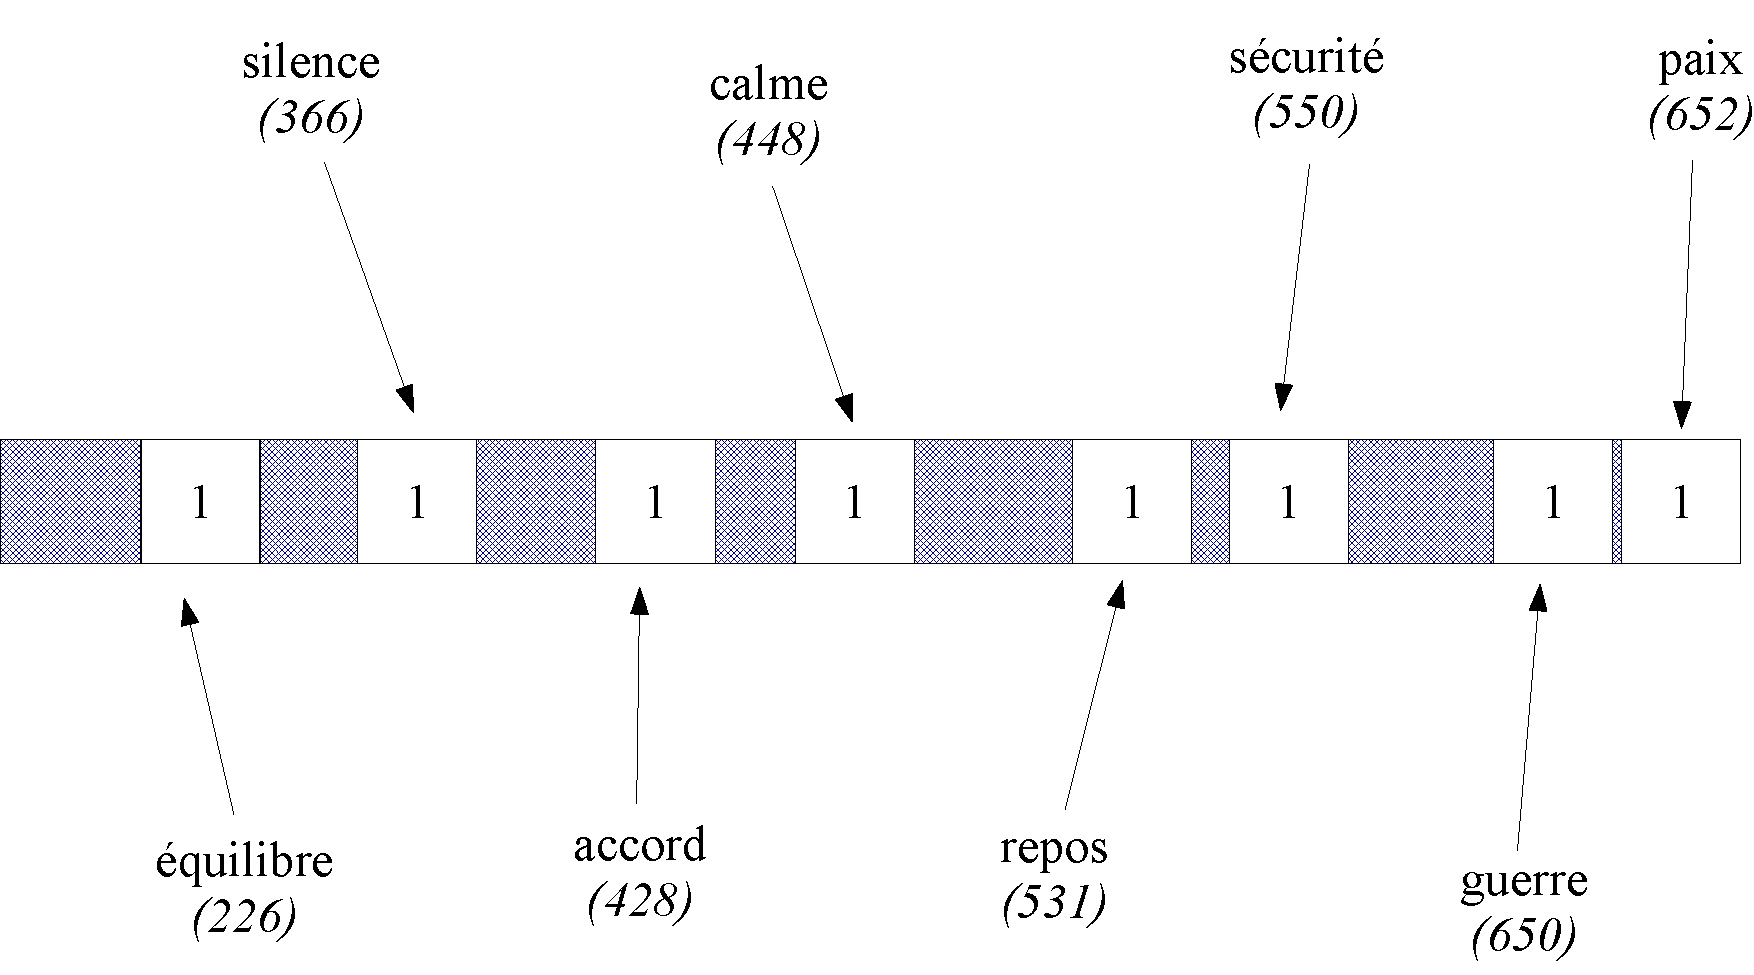
\includegraphics[width=10cm]{2_Etat-art/img/vect-paix-vect-sem}
      %\caption{Vecteur sémantique génératif du concept \cname{paix}
       % avant normalisation}
      %\label{Paix-vect-sem-gen}
    %\end{figure}
  %}
%\end{center}

%\subsubsection{Objets lexicaux}
%\label{sec:obj-lex-vect-sem}

%La base lexicale sémantique ne comporte qu'un seul type d'objets lexicaux~: le type \lexobj{item lexical}. Les \lexobj{items lexicaux}
%sont générés automatiquement à partir d'une version électronique de la partie index du thésaurus Larousse (cf. \ref{sec:thes-index}). Pour
%chaque entrée, on construit un \lexobj{item lexical} dont les caractéristiques sont~:

%\begin{itemize}
%\item \textbf{identifiant}~: l'entrée du thésaurus;
%\item \textbf{morphologie}~: composée des \emph{catégories
   % grammaticales} (\emph{nom, pronom, adjectif, adverbe, etc.}), du
  %\emph{genre} (\emph{masculin, féminin, neutre}) et du nombre
  %(\emph{singulier, pluriel}) tels que les donne le thésaurus;
%\item \textbf{vecteur sémantique}~: la somme vectorielle normée des
 % vecteurs génératifs correspondant aux concepts énoncés par le
 % thésaurus pour l'entrée. Les \index{vecteurs! sémantiques}vecteurs
 % sémantiques fusionnent donc l'ensemble des sens des mots.
%\end{itemize}

%Ce choix de construction, un seul objet lexical par item, ne permet
%donc pas une réelle désambiguïsation, en tout cas dans le sens que
%l'on entend habituellement qui est un choix (ou une préférence) parmi
%plusieurs solutions possibles. Nous allons le voir maintenant avec
%l'analyse sémantique, le sens global du texte émerge grâce aux
%vecteurs et à la contextualisation faible.

%Si nous prenons l'exemple de \lexItem{botte} dont la définition
%extraite du thésaurus est \sentence{\#nom commun\# sports,
 % agriculture, enseignement, herbes\_et\_fougères, pluie}, nous avons~:

%\begin{itemize}
%\item \textbf{identifiant}~: botte;
%\item \textbf{morphologie}~: nom commun;
%\item \textbf{vecteur sémantique}~: $V($\cname{sports}$) \vecadd
 % V($\cname{agriculture}$) \vecadd V($\cname{enseignement}$) \vecadd
 % V($\cname{herbes\ et\ fougères}$) \vecadd V($\cname{pluie}$)$
%\end{itemize}

%Si nous prenons l'exemple de \lexItem{manger} dont la définition
%extraite du thésaurus est \sentence{\#v\# prodigalité gloutonnerie
 % difficulté nutrition dents creux \#nom commun\# repas}, nous avons~:

%\begin{itemize}
%\item \textbf{identifiant}~: manger;
%\item \textbf{morphologie}~: v, nom commun;
%\item \textbf{vecteur sémantique}~: $V($\cname{prodigalité}$) \vecadd
 % V($\cname{gloutonnerie}$) \vecadd V($\cname{difficulté}$) \vecadd
 % V($\cname{nutrition}$) \vecadd V($\cname{dents}$)\vecadd
 % V($\cname{creux}$)\vecadd V($\cname{repas}$)$
%\end{itemize}

%\subsection{Analyse sémantique de textes en remontée-redescente grâce aux vecteurs sémantiques}
%\label{sec:an-sem-VS}

%\index{analyse sémantique! par remontée-redescente!
%(vecteurs sémantiques)}

%\subsubsection{Algorithme}

%L'analyse sémantique des textes en remontée-redescente grâce aux
%vecteurs conceptuels\index{vecteurs! conceptuels} est définie par les
%algorithmes \ref{algo:AS-VS1} et \ref{algo:AS-VS2}.

%\begin{algorithm}[h]
  %\Entree{vecteur sémantique $V_{contexte}$, $A$ arbre
   % morpho-syntaxique du texte, seuil $s$} \Sortie{vecteur sémantique
    %du texte}
  
  %Vecteur $V$ = analyse ($V_{contexte}$, A.racine)
  
  %\Repeter{(\dang{$V$}{$V_2$}<$s$)}{
   % Vecteur $V_2$ = $V$\\
    %$V$ = analyse\_VS($V_{contexte}$, A.racine)} \Retour $V$
%\caption{analyse~: algorithme d'analyse sémantique avec les vecteurs sémantiques}
  %\label{algo:AS-VS1}
%\end{algorithm}

%Cet algorithme \ref{algo:AS-VS1} est aussi utilisé pour une analyse
%sémantique avec les vecteurs conceptuels\index{vecteurs! conceptuels}
%(cf. \ref{sec:an-sem-VC}) avec un appel à analyse\_VC au lieu d'un
%appel à analyse\_VS.

%\begin{algorithm}[h]
  %\Entree{vecteur sémantique $V_{contexte}$, n\oe ud N}
  %\Sortie{vecteur sémantique du sous-arbre de N} \Si{N est une
    %feuille}{ \Si{N.item.estUnMotVide()}{ N.vecteur=$V_{\veczero}$}
    %\Sinon{N.vecteur= vecteur(N.item)} \Si{N.estGouverneur}{ N.vecteur
      %= $2\vecptt$N.vecteur } \Retour{N.vecteur} } \Sinon{
   % $V = \veczero$\\
    %\Pour{chacun des fils $f_i$ de N}{
      %$V = V + analyse(V_{contexte}, f_i)$\\
      %N.vecteur=norm(V) } }
%\caption{analyse\_VS~: algorithme d'analyse sémantique avec les vecteurs sémantiques}
  %\label{algo:AS-VS2}
%\end{algorithm}

%\subsubsection{Principe}

%L'analyse sémantique des textes grâce aux vecteurs
%sémantiques\index{vecteurs! sémantiques} est basée sur le principe
%suivant. Dans une première phase, les feuilles se voient affectées
%d'un vecteur d'idées\index{vecteurs! d'idées} correspondant à celui de
%l'item correspondant. Ce vecteur est contextualisé par un vecteur
%contexte. Dans le cas général, ce vecteur est le vecteur nul,
%toutefois si on possède des informations sur le thème du texte on peut
%utiliser un vecteur contexte plus approprié. Ensuite, une remontée
%vers le sommet de l'arbre est effectuée. Les vecteurs de chaque n\oe
%ud sont calculés à partir des vecteurs de leurs fils et de
%pondérations fonction de leur rôle syntaxique. Le vecteur de chaque
%n\oe ud est ainsi calculé récursivement jusqu'au sommet de l'arbre. Ce
%vecteur possède les idées contenues dans tout mots du textes. À ce
%moment du calcul, il n'y a eu, dans le cas général, aucune
%contextualisation. Le vecteur du sommet de l'arbre contient donc les
%idées pertinentes du textes mais aussi beaucoup de bruit. Il s'agit
%donc de faire passer aux feuilles de l'arbre le vecteur contexte
%global et ensuite de sélectionner les idées les plus pertinentes de
%chaque vecteur grâce à une contextualisation faible. On effectue
%ensuite une nouvelle remontée toujours avec les pondérations
%précédentes. Une analyse sémantique nécessite un certain nombre de
%remontées-redescentes tant que le vecteur conceptuel ne s'est pas
%relativement stabilisé c'est-à-dire tant que la distance angulaire
%entre deux vecteurs du sommet calculée n'est pas inférieure à un
%certain seuil $s$.

%\index{analyse sémantique! par remontée-redescente!
%(vecteurs sémantiques)}

%\begin{figure}[h]
  

  %\centering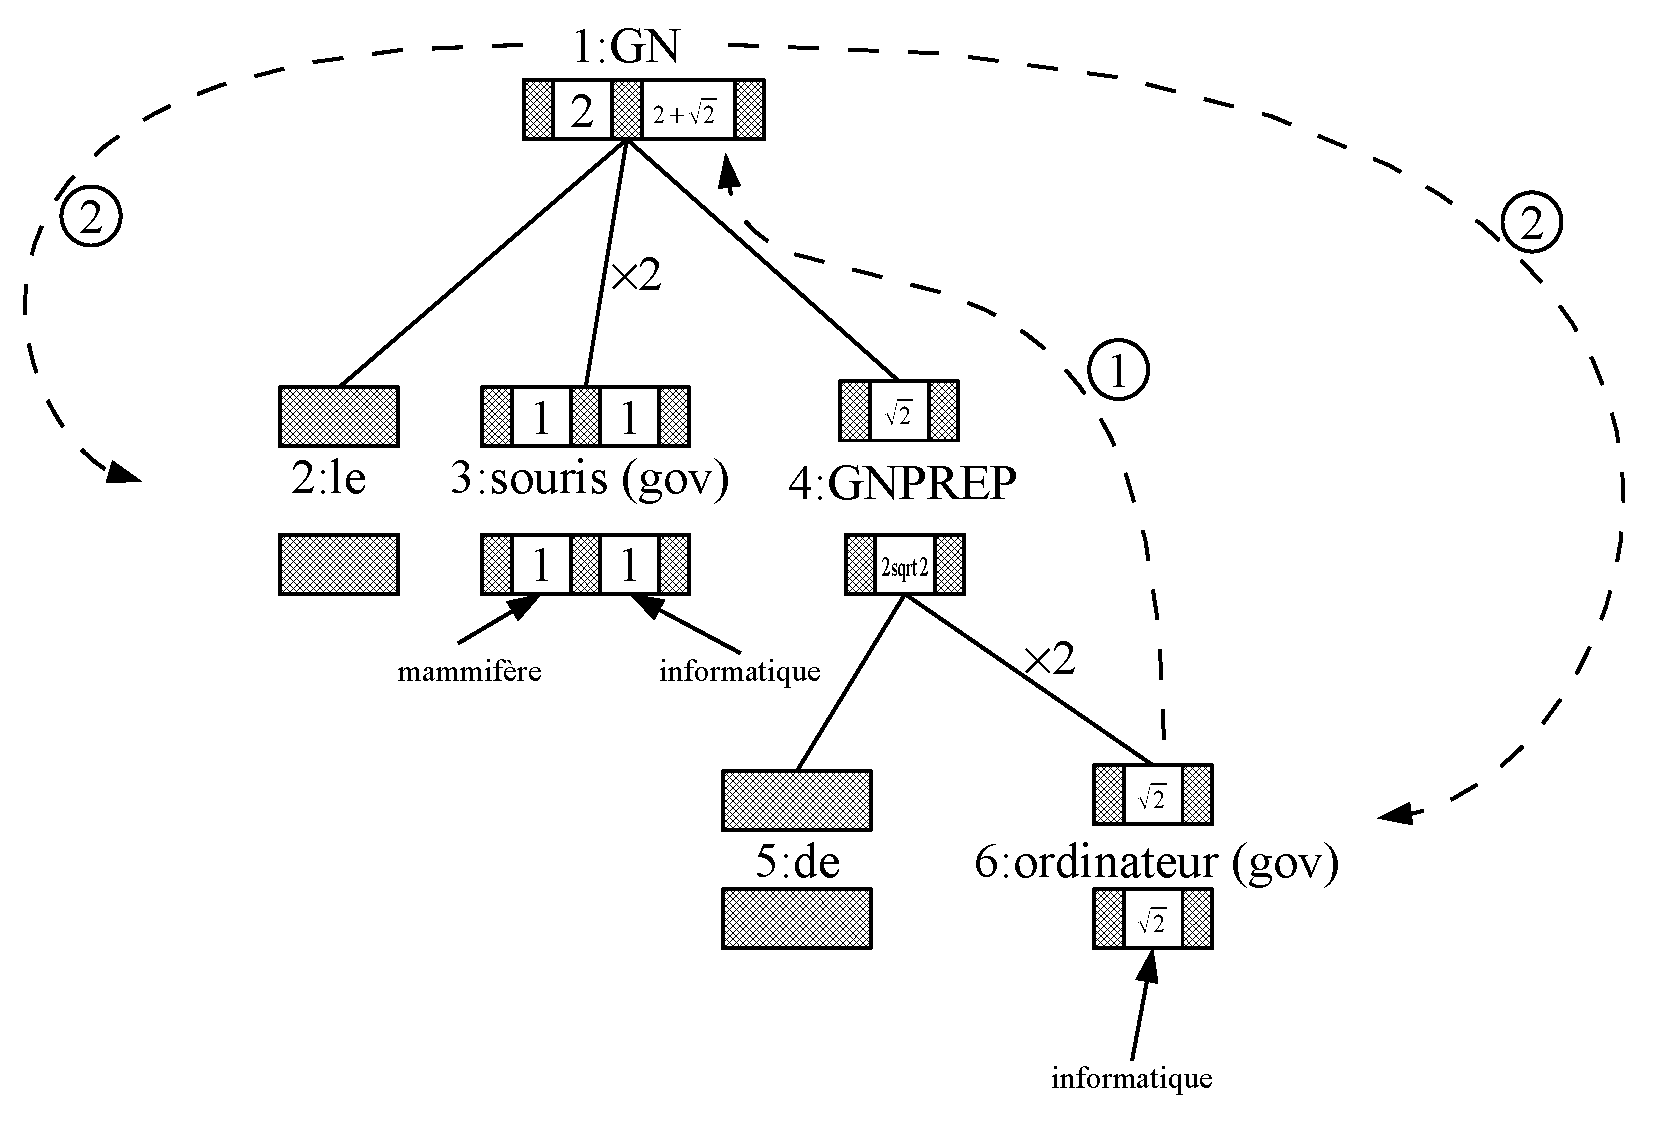
\includegraphics[width=16cm]{2_Etat-art/img/an-sem-VS-souris-de-lordi}
%\caption{Exemple d'analyse sémantique grâce aux vecteurs sémantiques}
%\label{fig:an-sem-VS}
%\end{figure}

%En général le nombre de remontées-descentes est inférieur à 3, cette
%méthode est ainsi très légère en temps de calcul. L'expérience sur la
%catégorisation que nous présentons en \ref{sec:categ-doc} et qui
%concernait 5222 dépêches d'agences a duré à peu près une demi-heure
%toutes opérations comprises (analyse morpho-syntaxique, analyse
%sémantique puis catégorisation des documents) sur un ordinateur
%standard (Pentium IV, 2.4 Ghz, 512 Mo RAM, 4771 bogomips).

%\subsubsection{Exemple}

%La figure \ref{fig:an-sem-VS} présente un petit exemple d'analyse
%sémantique grâce aux vecteurs sémantiques\index{vecteurs! sémantiques}
%avec le segment textuel \sentence{la souris d'ordinateur.}. Les
%feuilles correspondant aux mots vides de sens (\lexItem{le},
%\lexItem{de}) se voient affectées d'un vecteur vide tandis que les
%autres se voient affectées du vecteur correspondant à l'item de la
%feuille dans la base. Le vecteur du n\oe ud $4$ est constitué de la
%somme vectorielle pondérée des vecteurs des n\oe uds $5$ et $6$. Le
%n\oe ud $6$ est gouverneur, il a donc un poids supérieur ($2$ dans
%l'exemple). De même, pour le calcul du n\oe ud $1$, le vecteur du n\oe
%ud $3$ aura un poids prépondérant sur les vecteurs des n\oe uds $2$ et
%$4$. Le vecteur général du texte, ici $1$, est ensuite utilisé pour
%faire une contextualisation faible avec les vecteurs des feuilles de
%l'arbre. Le principe de la remontée est le même. On remarquera que le
%vecteur général du texte s'oriente vers une idée
%d'\cname{informatique} dès la première remontée dans cet exemple et
%que la contextualisation ne pourra qu'accentuer le phénomène.

%\subsection{Exemple d'application des vecteurs sémantiques~: catégorisation automatique de documents}\label{sec:categ-doc}

%Dans sa thèse \cite{jaillet2005}, Simon Jaillet étudie diverses
%méthodes de \emph{catégorisation de documents}. \index{Jaillet Simon}
%Deux voies sont suivies. Dans une première, il exploite des méthodes
%de fouille de données (motifs séquentiels) tandis que dans une
%seconde, il utilise des méthodes issues du TALN pour représenter les
%documents.  On trouve ici l'une des applications les plus abouties
%utilisant les vecteurs sémantiques\footnote{Simon Jaillet utilise tout
  %au long de sa thèse le terme \emph{vecteur conceptuel} mais il
  %serait plus juste d'employer \emph{vecteur
    %sémantique}.\index{Jaillet Simon}}.\index{vecteurs! sémantiques}

%Ce type de vecteurs est particulièrement creux puisque pour un terme,
%on trouve au maximum une demi-douzaine de composantes non vides sur
%les 873 que comptent les \index{vecteurs! sémantiques} vecteurs
%sémantiques. Cette caractéristique favorise la discrimination entre
%vecteurs et fait ainsi de la catégorisation de textes une application
%qui leur est particulièrement destinée.

%Deux expériences sont menées avec les vecteurs
%sémantiques.\index{vecteurs! sémantiques} Il s'agit dans les deux cas
%de retrouver automatiquement de quelles catégories sont issus les
%textes d'un corpus pré-catégorisé par des spécialistes.  Ce corpus
%comprend 28 catégories qui vont des \emph{nouvelles internationales} à
%l'\emph{aéronautique} en passant par les \emph{finances} ou les
%\emph{télécoms}. 8022 dépêches d'agences de presse sont réparties
%entre ces catégories. Pour l'expérience, elles sont constituées en un
%jeu d'entraînement pour la méthode de catégorisation de 2800 articles
%et un jeu de test de 5222 articles.  Dans la première expérience, un
%seul vecteur permet de représenter l'ensemble d'un texte tandis que
%dans la seconde dite \emph{méthode des sous-textes}, il est représenté
%par trois vecteurs sémantiques~: \index{vecteurs! sémantiques} un
%premier pour l'introduction, un deuxième pour la conclusion et un
%dernier pour le corps. Quelle que soit la méthode de catégorisation
%utilisée (\emph{méthode des deux écarts}, \emph{Support Vector
 % Machine}\footnote{Support Vector machine (ou SVM) \cite{boser92} est
  %un algorithme d'apprentissage qui construit un hyperplan optimisant
  %la frontière entre des cas positifs et des cas négatifs pour une
  %tâche donnée.}), la méthode des sous-textes s'avère meilleure. En
%effet, pour des textes courts les résultats sont quasi-identiques
%(gain sur le $F_{score}$ inférieur à 1\%) tandis que sur les textes
%plus longs, qui se prêtent donc mieux à cette méthode, le gain est net
%(de l'ordre de + 4\%).

%\subsection{Limites de l'approche "vecteurs sémantiques" pure}

%Deux critiques semblent pouvoir être faites concernant les vecteurs
%sémantiques. \index{vecteurs! sémantiques}La première concerne en
%particulier leur construction.  Elle est basée sur une seule source,
%la version électronique du thésaurus Larousse, qui comme toutes les
%autres peut difficilement couvrir l'ensemble du lexique. En
%particulier, aucun nom propre n'y figure et bien entendu aucun
%néologisme ce qui peut entraîner des difficultés pour véritablement
%faire émerger la thématique associée à certains textes comme
%\sentence{Renault a affiché des résultats record en 2004 et prévoit
 % une dégradation de sa rentabilité en 2005 dans un environnement
 % moins favorable, marqué notamment par un impact accru de la hausse
 % des matières premières.} qui ne contient aucune information autre
%que \lexItem{Renault} sur le domaine \emph{automobile}. Il faut bien
%comprendre ici que le problème ne vient pas de l'utilisation du
%thésaurus Larousse en particulier mais du fait qu'il n'y a qu'une
%seule source.

%La deuxième critique que l'on pourrait faire des vecteurs
% sémantiques\index{vecteurs! sémantiques} concerne ce qu'on appelle l'\emph{hybridation vectorielle}. En effet, fusionner l'ensemble des
%acceptions d'un terme peut conduire à faire émerger des idées qui ne coexistent pas dans le même sens. Par exemple, si on considère que
%l'item \lexItem{souris} a deux acceptions l'une \annotation{animal} caractérisée par des idées de \cname{animal}, \cname{gris},
%\cname{fromage} et l'autre \lexItem{souris} d'\annotation{ordinateur} caractérisée, elle, par \cname{informatique}, dans une phrase comme
%\sentence{Il posa son pain au fromage près de la souris de son ordinateur}, les idées émergentes pour le vecteur associé à
%\lexItem{souris} seront \cname{informatique} et \cname{gris}, ce qui ne correspond pourtant pas à un sens de l'item.

%\subsection{La méthode mixte~: une approche combinant des vecteurs sémantiques et distributionnels}
%\label{sec:vect-sem-mixte}

%Pour pallier ces limites, \cite{jaillet2005} introduit la méthode mixte. Il s'agit de tirer profit à la fois des avantages de la représentation sous forme de vecteurs saltoniens (cf. \ref{sec:repr-salt-et-deriv}) et des avantages de la représentation sous forme de vecteurs sémantiques. \index{vecteurs! sémantiques}Comme le note l'auteur, \sentence{la représentation statistique permet de mettre en évidence le vocabulaire discriminant tandis que la représentation conceptuelle permet, quant à elle, d'obtenir une vision globale du texte en projetant ce dernier sur un ensemble de concepts.}

% En pratique, les vecteurs utilisés pour représenter les textes sont définis comme la concaténation du vecteur statistique et du vecteur sémantique. Dans le vecteur résultant, les composantes issues du vecteur distributionnel sont largement plus nombreuses que celles issues du vecteur sémantique. On peut estimer le rapport en fonction du nombre d'items dans le corpus comme pouvant aller de 1 à 10 voire de 1 à 100 dans un cas extrême (environ 1000 concepts pour la représentation sous forme de \index{vecteurs! sémantiques}vecteurs sémantiques contre 100000 items en langue). Il faut donc utiliser une méthode de catégorisation qui tienne compte de ce phénomène afin que les composantes "idées" ne soient pas complètement noyées dans les composantes statistiques. Des méthodes comme les SVM ou les réseaux de neurones donnent à chacune des dimensions une importance qui lui est propre.

%Grâce à la méthode mixte, les termes inconnus de la base de données vectorielle se voient affectés d'un vecteur dont les composantes ne sont pas toutes vides et ils participent ainsi à la représentation globale du texte.

% Sur le corpus en français présenté dans la partie \ref{sec:categ-doc}, les résultats obtenus par la méthode mixte ($F_{score} = 0.51$) se voient largement améliorés, que ce soit par rapport aux résultats obtenus avec les vecteurs sémantiques\index{vecteurs! sémantiques} purs ($F_{score} = 0,404$; $+26\%$) ou par rapport à ceux obtenus en utilisant les vecteurs saltoniens purs ($F_{score} = 0,486$; $+4,9\%$). Ces expériences montrent que l'utilisation de représentations conceptuelles permet d'améliorer la représentation textuelle puisqu'elle atténue les effets de la polysémie du vocabulaire des textes, contrairement aux vecteurs saltoniens purs qui n'envisagent que les formes de surface.

%Il convient de noter que les résultats en termes qualitatifs peuvent
%paraître modestes avec un $F_{score} = 0.51$ mais nous n'avons
%présenté ici que l'expérience menée sur le français. Dans cette expérience, les catégories se sont avérées souvent très générales et leurs intersections non vides. Ainsi, il n'est pas rare de trouver un texte dans une catégorie alors qu'il aurait sans doute pu appartenir à une ou plusieurs autres. En revanche, dans l'expérience menée sur l'anglais, même sans analyse morpho-syntaxique préalable puisque l'équipe n'a pas actuellement à sa disposition un équivalent à SYGFRAN pour cette langue, les catégories sont bien mieux définies, ce qui se ressent fortement sur les résultats obtenus avec les trois méthodes. L'expérience a été menée sur le corpus en anglais \emph{Reuters-21578}. Il comporte 12902 dépêches qui ont été réparties en 9603 destinées au corpus d'entraînement et 3299 au corpus de test. 9624 items lexicaux ont été extraits de ce premier corpus pour constituer \index{espace vectoriel! saltonien} l'espace vectoriel saltonien. Les vecteurs sémantiques\index{vecteurs! sémantiques} anglais ont été obtenus grâce à la version électronique du thésaurusRoget disponible en ligne\footnote{\url{ftp://ibiblio.org/pub/docs/books/gutenberg/etext91/roget13.zip}}.

%Ici encore, les résultats obtenus par la méthode mixte ($F_{score} =
%0,86$) se voient largement améliorés, que ce soit par rapport aux
%résultats obtenus avec les \index{vecteurs! sémantiques} vecteurs
%sémantiques ($F_{score} = 0,771$; $+11,54\%$) ou avec les vecteurs
%saltoniens ($F_{score} = 0,84$; $+ 2,38\%$).

\section{Descripteurs textuels dans VideoSense : les vecteurs conceptuels} \label{sec:vectconcept}

Dans le cadre du projet VidéoSense, nous utilisons ce modèle, proche dans sa
conception de la théorie componentielle, qui est l'héritier direct de
celui des proto-vecteurs d'idées présenté en \ref{sec:chauche}. Ainsi,
il postule que le sens des termes peut être calculé à partir d'un
ensemble de concepts. Dans le cadre de videosense, nous étudions 2 modes de construction : un premier basé sur un ensemble de concepts connus \textit{a priori}, un second basé sur un ensemble de concepts émergents.

Pour notre première expérience, nous
nous reposons sur des thésaurus généraux. Ces thésaurus ont
pour but d'organiser les termes du lexique en fonction des idées
qu'ils véhiculent. Ainsi, pour un certain nombre de langues, il existe
des thésaurus qui décrivent le lexique en fonction d'une
classification mise au point pour cet exercice.

\subsection{Les thésaurus}
\label{sec:thes-larousse}

\subsubsection{Généralités}

Un thésaurus comporte un ensemble de concepts censés permettre de
décrire l'ensemble des idées exprimables en langue (\emph{hypothèse du
  thésaurus}). Un thésaurus n'est pas à proprement parlé d'inspiration
componentielle, puisque les premiers sont antérieurs de près d'un
siècle à cette théorie, mais s'en rapprochent fortement.  Le but d'un
thésaurus est, selon les auteurs de \cite{Thesaurus1992},
\sentence{d'explorer à partir d'une idée l'univers des mots qui s'y
  rattachent et de trouver des idées à partir des mots liées à une
  notion}.

Un thésaurus est le résultat d'un long processus de tri des items
lexicaux d'une langue donnée. Ce tri conduit à la constitution d'une
hiérarchie qui diffère donc suivant les idées importantes dans le
vocabulaire de telle ou telle société (donc les idées importantes dans
telle ou telle société).  Ainsi, le thésaurus du français se
différencie de celui de l'anglais beaucoup plus raffiné, par exemple,
sur des notions comme celle qui touchent au fait religieux.

De même, les thésaurus s'adaptent aux évolutions de la société. Ainsi,
comme les rédacteurs du thésaurus Roget le notent dans la préface de
la version datant de 1987 \cite{Roget1987} \sentence{Cette version a
  été rendue nécessaire par l'extension sans précédent du vocabulaire
  de l'anglais durant les années 1980, qui reflète les principaux
  changements d'ordre scientifique, culturel ou social.  Les
  découvertes et les inventions dans le monde des sciences, de la
  médecine et des technologies ont fait apparaître des termes comme
  acid rain, AIDS, genetic fingerprinting, nuclear winter,
  \ldots\footnote{pluies acides, SIDA, empreintes génétiques, hiver
    nucléaire, \ldots}}.

Le thésaurus Larousse, que nous allons présenter plus particulièrement
ici, est inspiré du thésaurus de Roget paru en Grande-Bretagne au
milieu du XIXe siècle \cite{Roget1852}. Il est constitué de trois
parties : (1)~\emph{organisation des idées} qui constitue la
hiérarchie du thésaurus; (2)~la partie \emph{thésaurus} proprement
dite qui permet à partir d'idées de trouver des mots dans le même
thème et (3)~la partie \emph{index} qui permet de trouver les idées
associées aux mots.

\subsubsection{Le thésaurus Larousse}

\paragraph{La partie \emph{Organisation des idées} : la hiérarchie
  Larousse}
\label{sec:thes-hierarchie}

Ce thésaurus est basé sur une classification organisée selon une
structure hiérarchique d'arbre qui comporte 5 niveaux :

\begin{itemize}
\item niveau 0 : 1 concept (\cname{c0:omega}), la racine de l'arbre.
  Il faut noter que ce concept n'existe pas explicitement dans la
  hiérarchie, nous l'avons rajouté pour disposer d'un véritable arbre
  hiérarchique.
\item niveau 1 : 3 concepts (\cname{c1:le monde}, \cname{c1:l'homme},
  \cname{c1:la société})
\item niveau 2 : 26 concepts
\item niveau 3 : 95 concepts
\item niveau 4 : 873 concepts, les feuilles de l'arbre.
\end{itemize}

Afin de les distinguer suivant leur niveau de hiérarchie, nous notons
ici les concepts par un \emph{c} concaténé au numéro de niveau du
concept, à deux points puis enfin au nom du concept. Par exemple, le
concept de niveau 0 oméga est noté \cname{c0:omega}, le concept de
niveau 4 existence est noté \cname{c4:existence}. Pour des raisons de
clarté, nous omettrons souvent cette convention d'écriture en ce qui
concerne les niveau 4 de la hiérarchie (\cname{c4:existence} sera
alors noté \cname{existence}).

Les concepts de niveau 4 se succèdent, quand cela s'y prête, en
fonction des domaines auxquels ils appartiennent par paires de notions
proches, corrélatives ou opposées. Nous avons donc des contraires
comme \cname{existence} ($1$) et \cname{inexistence} ($2$),
\cname{honneur} ($641$) et \cname{discrédit} ($642$), qui se suivent
ainsi que des termes proches thématiquement comme \cname{amour}
($600$) ou \cname{caresse} ($601$).
                  %, \cname{passion} ($602$).
La figure \ref{fig:hierarchie-larousse} présente un extrait de cette
hiérarchie.
% La hiérarchie complète de \cite{Thesaurus1992} se trouve
%en annexe \ref{Annexe:hierarchieLarousse}.


Selon les auteurs, la hiérarchie du thésaurus \sentence{(couvre)
  méthodiquement l'ensemble des champs notionnels possibles (de la
  langue)}.  Ainsi, l'ensemble des concepts de niveau 4 permettrait de
définir la globalité des termes du lexique. C'est sur cette hypothèse,
que nous appelons \emph{hypothèse du thésaurus}, que reposent nos
expérimentations.

\begin{figure} [h]
 % \hrulefill
    \begin{flushleft}
      \footnotesize{ \algolinenonum{0.2}{\cname{0 omega}}
        \algolinenonum{0.4}{\cname{1 Monde}}
        \algolinenonum{0.6}{\ldots} \algolinenonum{0.6}{\cname{2
            Espace}} \algolinenonum{0.6}{\cname{2 Temps}}
        \algolinenonum{0.8}{\cname{2 Temps et Durée}}
        \algolinenonum{0.8}{\cname{3 Date et Chronologie}}
        \algolinenonum{1}{\cname{4 Passé}} \algolinenonum{1}{\cname{4
            Présent}} \algolinenonum{1}{\cname{4 Futur}}
        \algolinenonum{1}{\ldots} \algolinenonum{0.8}{\cname{3
            Évolution et Histoire}} \algolinenonum{0.8}{\ldots}
        \algolinenonum{0.6}{\cname{2 Matière}}
        \algolinenonum{0.6}{\cname{2 Vie}} \algolinenonum{0.6}{\ldots}
        \algolinenonum{0.4}{\cname{1 Homme}}
        \algolinenonum{0.6}{\cname{2 Être Humain}}
        \algolinenonum{0.6}{\cname{2 Corps et Vie}}
        \algolinenonum{0.8}{\cname{3 Corps}}
        \algolinenonum{1}{\cname{4 Tête}} \algolinenonum{1}{\cname{4
            Membres}} \algolinenonum{1}{\cname{4 Main}}
        \algolinenonum{1}{\cname{4 Pied} }
        \algolinenonum{0.8}{\cname{3 Fonctions vitales}}
        \algolinenonum{0.8}{\ldots} \algolinenonum{0.6}{\cname{2 Corps
            et Perceptions}} \algolinenonum{0.6}{\cname{2 Esprit}}
        \algolinenonum{0.6}{\ldots} \algolinenonum{0.4}{\cname{1
            Société}} \algolinenonumnoreturn{0.6}{\ldots} }
\end{flushleft}
\caption{Extrait de la hiérarchie du thésaurus Larousse
  \cite{Thesaurus1992}\label{fig:hierarchie-larousse}}
%\hrulefill
\end{figure}

\paragraph{La partie \emph{Thésaurus} : des idées aux mots}
\label{sec:thes-part}

Cette section est constituée pour permettre au lecteur de trouver des
mots en fonctions d'idées.  Cette partie du thésaurus comporte 873
articles qui correspondent à chacun des concepts de niveau 4. Les
notions traitées sont elles-mêmes divisées en paragraphes ordonnés
selon les catégories grammaticales.  Chacun de ces paragraphes
regroupe des mots proches sémantiquement qu'il est possible de
parcourir grâce à des renvois vers des notions communes permettant
ainsi de faciliter les associations d'idées ou la recherche
d'expressions les plus pertinentes possible.

\paragraph{La partie \emph{Index} : des mots aux idées}
\label{sec:thes-index}

Cette dernière partie est sans nul doute la plus utilisée dans le
cadre des vecteurs d'idées puisqu'elle permet de retrouver à partir
d'un mot les idées, les thèmes qui lui sont associés. On y trouve, par
exemple, que \lexItem{échelle} est un \emph{nom commun} et que ses
concepts associés sont \cname{musique}, \cname{montée} et
\cname{mesure}. On voit donc que cette partie du thésaurus permet
facilement de construire une base de données de vecteurs, une fois les
concepts eux-mêmes munis d'un vecteur (vecteurs génératifs
cf.~\ref{sec:famGen}). On peut toutefois regretter que les
distinctions entre les sens ne soit pas bien marquées. Si on reprend
l'exemple d'\lexItem{échelle} les sens \annot{échelle}{escalier} et
\annot{échelle}{musique} sont, par exemple, clairement fusionnés.

\begin{center}
  \begin{figure}%[H]
    
    \emph{fable} (\emph{nom fem}) : \cname{morale}, \cname{mensonge},
    \cname{représentation}, \cname{récit}
    
    \emph{million} (\emph{nom masc}) : \cname{multitude},
    \cname{mille}
    
    \emph{échelle} (\emph{nom fem}) : \cname{musique}, \cname{montée}
    et \cname{mesure}
    
    \emph{pêcher} (\emph{verbe}) : \cname{pêche}

 \caption{Exemple de quelques termes extraits du thésaurus Larousse
   \cite{Thesaurus1992}}
  \end{figure}
\end{center}

%Nous venons de le voir, les \index{vecteurs! sémantiques} vecteurs
%sémantiques permettent de représenter une thématique globale des
%segments textuels. Un de leurs grands avantages est leur rapidité dans
%le traitement des opérations ainsi qu'une relativement faible
%importance de la taille de la base de données. Toutefois, ils peuvent
%s'avérer limités pour des traitements plus évolués à cause de leurs
%limites en ce qui concerne la couverture lexicale ou l'hybridation de
%vecteurs. L'équipe a ainsi commencé à mettre au point les vecteurs
%conceptuels.\index{vecteurs! conceptuels}

Les vecteurs conceptuels\index{vecteurs! conceptuels} visent à une
représentation ainsi qu'à des traitements plus fins du sens des
segments textuels. Ainsi, nous ne considérons pas, comme dans les
vecteurs sémantiques,\index{vecteurs! sémantiques} un seul objet
lexical pour représenter le sens d'un terme mais plusieurs~: les
\lexobj{lexies}. L'objet lexical \lexobj{item lexical} correspond au
terme et fusionne les informations des différentes lexies. Ces lexies
sont constituées à partir d'un apprentissage permanent utilisant des
dictionnaires à usage humain. Ce mode de construction de la base de
données vectorielles permet d'assurer une certaine couverture
lexicale.

%\subsection{Objectifs visés} \label{sec:objectifs-vises}

%Les objectifs des vecteurs conceptuels\index{vecteurs! conceptuels}
%sont hétérogènes. Ils visent à mettre au point ou améliorer toute
%application dans laquelle une représentation fine du sens pourrait
%s'avérer utile. On peut ainsi citer la \emph{recherche d'informations}
%pour laquelle préciser un sens particulier pour un terme peut
%permettre d'affiner les résultats, la \emph{traduction automatique} où
%elle peut permettre de trouver le meilleur équivalent possible pour la
%langue cible. Dans la phrase \sentence{l'élève a fait le devoir que
%  lui avait donné la maîtresse.}, le substantif \lexItem{devoir}
%devrait être traduit en anglais par \lexItem{homework} et non par
%\lexItem{duty} qui a plutôt un sens d'\lexItem{obligation morale}.

\subsection{Vecteurs génératifs~: origine et interdépendance des concepts}\label{sec:vect-gener-VC}

\index{vecteurs génératifs! de l'espace des vecteurs! conceptuels}
\index{vecteurs! conceptuels} Les vecteurs génératifs sont les seuls
vecteurs conceptuels à être construits manuellement.  Leur
construction est basée sur l'hypothèse forte que les concepts ne sont
pas indépendants les uns des autres.

Pour la construction de nos vecteurs génératifs, nous avons choisi un
ensemble de concepts issus du thésaurus Larousse \cite{Thesaurus1992}
que nous avons présenté en \ref{sec:thes-larousse}. L'ensemble de
concepts considéré correspond à celui des 873 concepts de niveau 4 de
cette hiérarchie.  L'interdépendance des concepts se situe à deux
niveaux dans la construction des vecteurs génératifs~: au niveau
hiérarchique, c'est-à-dire en tenant compte de la place que le concept
a dans la hiérarchie (\emph{vecteurs génératifs hiérarchiquement
  augmentés}) et à un niveau transversal à cette hiérarchie
(\emph{vecteurs génératifs transversalement augmentés}).

\begin{figure}[h]
  
  \centering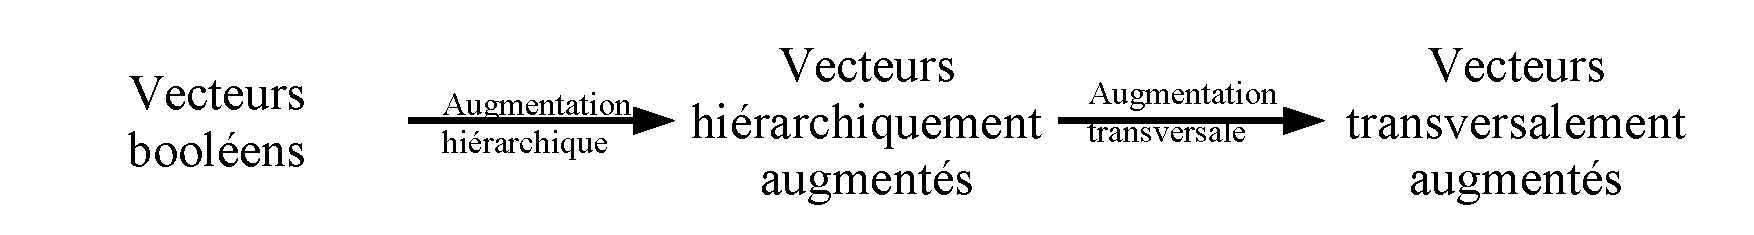
\includegraphics[width=16cm]{2_Etat-art/img/VG-VC}
\caption{Séquence d'opérations pour la construction des vecteurs génératifs}
\label{fig:VG-VC}
\end{figure}

\subsubsection{Interdépendance hiérarchique~: vecteurs génératifs
  hiérarchiquement augmentés}

\index{vecteurs génératifs! de l'espace des vecteurs! conceptuels}

Le point de départ de cette construction est un vecteur booléen. Le
vecteur booléen du concept i est le vecteur dont tous les éléments
sont à 0 sauf la composante i qui elle est à 1.  Cette construction
est simple et elle obtient souvent de bons résultats mais semble
inadéquate dans plusieurs cas.  Il paraît curieux que deux concepts
proches comme le sont \cname{guerre} et \cname{paix} partagent
quantitativement autant d'idées que \cname{paix} et
\cname{champignon}.  Nous l'avons déjà dit, les concepts ne sont
clairement pas indépendants et leurs vecteurs respectifs doivent en
tenir compte.  L'ensemble des concepts défini selon
\cite{Thesaurus1992} est hiérarchiquement ordonné selon un arbre (cf.
\ref{sec:thes-larousse}).  La construction des vecteurs génératifs est
basée sur cette structure et plus particulièrement sur la distance
ultramétrique \index{distance! ultramétrique} entre deux concepts.  Il
s'agit de la longueur du chemin minimal à parcourir dans l'arbre des
concepts pour aller d'un concept à l'autre.  Cette distance est
définie par:

\begin{equation}
\dum{C, C} = 0 
\end{equation}

\begin{equation}
\dum{C_{1}, C_{2}} = \min 
{\dum{Sup(C_{1}), C_{2}}+1 \brack
\dum{C_{1}, Sup(C_{2})}+1} 
\end{equation}

où $Sup(X)$ est le père du concept X. Par définition, on a $Sup
(racine(arbre)) = racine (arbre)$. Si nous nous référons à la figure
\ref{fig:hierarchie-larousse}, nous avons $\dum{t\hat{e}te,
  membre}=2$. Tous les concepts frères de tête sont à une distance
ultramétrique \index{distance! ultramétrique} égale à 2.  Nous avons
également $\dum{t\hat{e}te, corps}=1$,\\$\dum{t\hat{e}te, fonctions
  vitales}=3$ et $\dum{t\hat{e}te, pr\acute{e}sent}=8$. La valeur 8
est d'ailleurs la plus grande possible entre deux concepts de cette
hiérarchie puisque leur ancêtre commun le plus éloigné est la racine,
située au maximum à quatre niveaux au-dessus.

Grâce à cette \index{distance! ultramétrique} distance ultramétrique,
nous construisons les \emph{vecteurs génératifs hiérarchiquement
  augmentés}. Appelons $X_i$ le vecteur booléen correspondant au i-ème
concept de la base $\cal C$.  $Y_i$ est le vecteur conceptuel
hiérarchiquement augmenté défini par~:

\begin{equation}
Y_{i} =  X_{i} \vecadd \bigvecadd_{j=0}^{\dim(\cal C)} 
{\frac{1}{2^{\dum{C_{i}, C_{j}}}}} \times X_{j}
\end{equation}

Le vecteur original $X_i$ est ajouté afin que, de tous les vecteurs
$Y_j$, le plus proche de $X_i$ soit toujours $Y_i$. La figure
\ref{boolEtHierPaix} montre, pour \cname{paix}, le vecteur booléen et
le vecteur hiérarchiquement augmenté.

\begin{figure}[h]
  \rotatebox{-90}{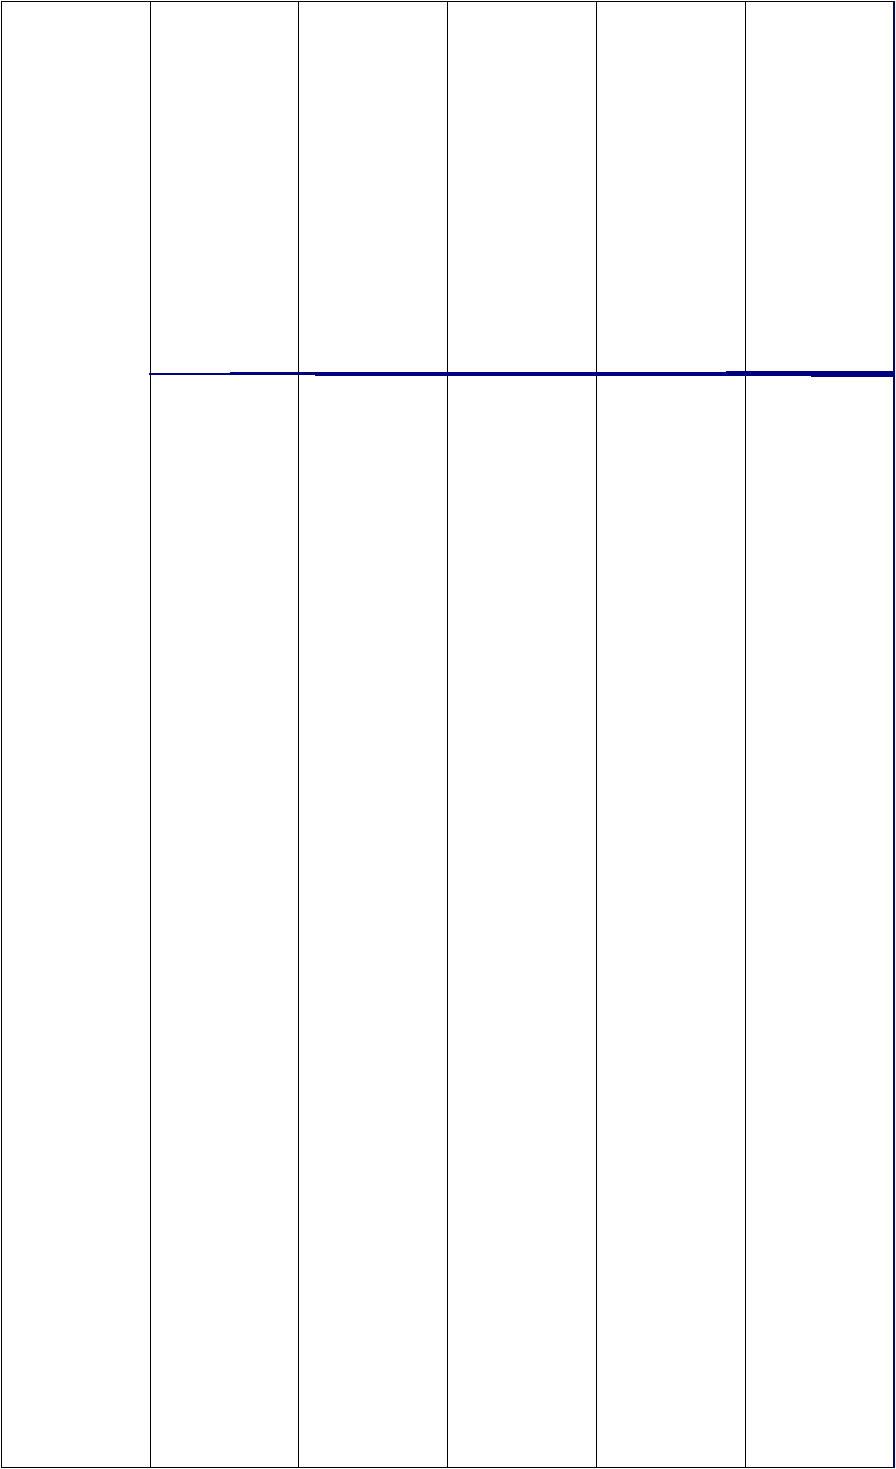
\includegraphics[height=8cm]{2_Etat-art/img/c4paix-l0}}
  \rotatebox{-90}{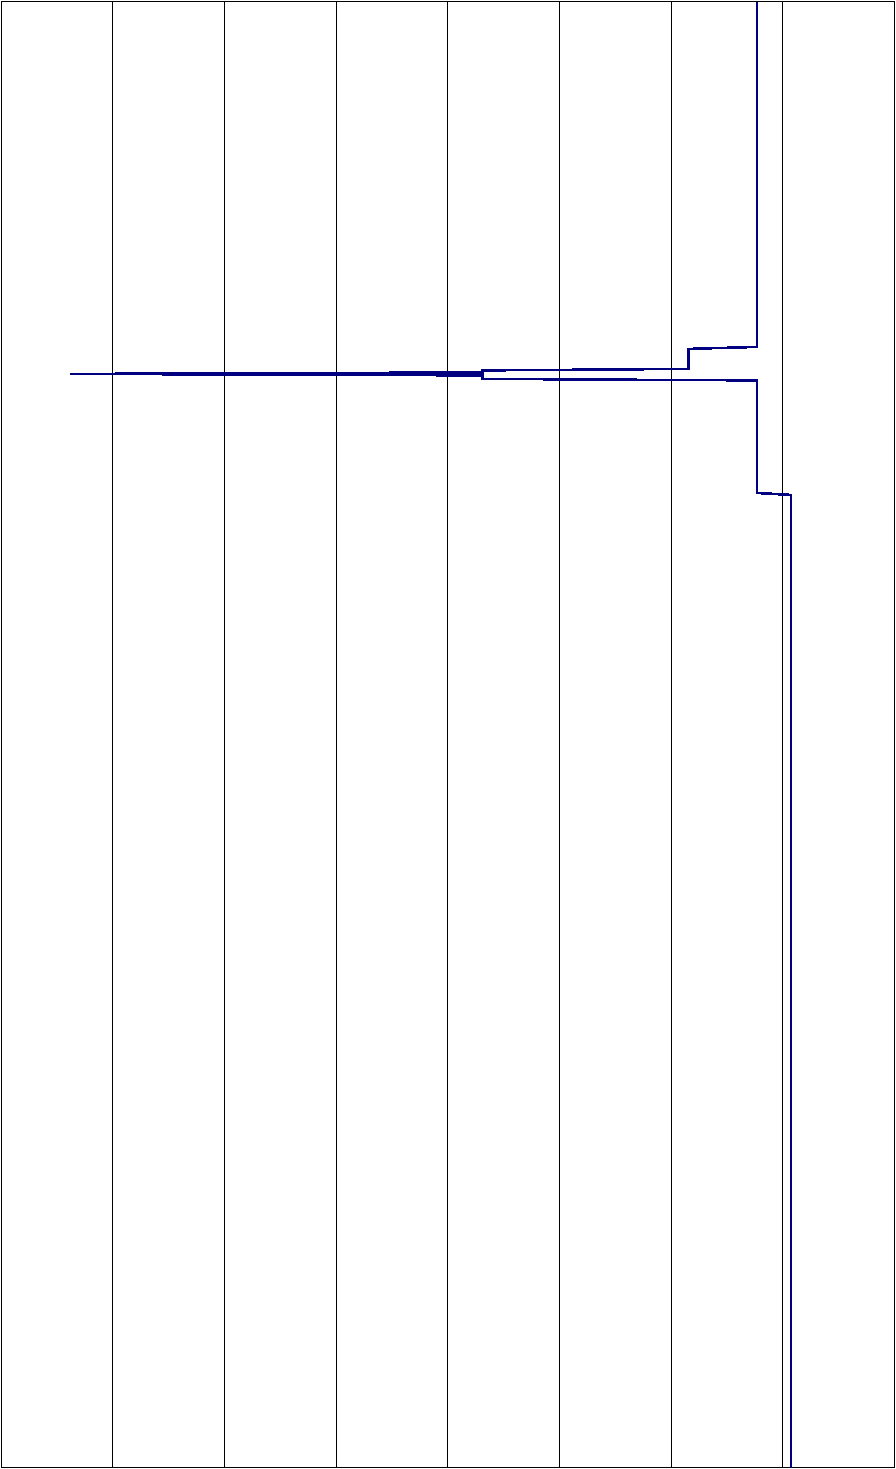
\includegraphics[height=8cm]{2_Etat-art/img/c4paix-l1}}
    \caption{Vecteur du concept \cname{paix} et vecteur hiérarchiquement augmenté du concept \cname{paix}}
    \label{boolEtHierPaix}
\end{figure}

\subsubsection{Interdépendance transversales~: vecteurs génératifs transversalement augmentés}
\index{vecteurs génératifs! de l'espace des vecteurs! conceptuels}

Bien qu'augmenter un vecteur par ses voisins améliore sa qualité, il
faut admettre que la hiérarchie des concepts n'est qu'une vue
particulière de la façon selon laquelle ils peuvent être organisés.
D'autres liens spécifiques peuvent être exhibés.  C'est le cas entre
\cname{champignon} et \cname{toxicité} ou \cname{gastronomie} par
exemple.  L'augmentation transversale d'un concept C est une opération
manuelle réalisée une seule fois, à des ajustements près, qui consiste
à énumérer les concepts relatifs à C qui ne sont pas représentés dans
la hiérarchie.  Le nouveau vecteur est appelé \emph{vecteur
  transversalement augmenté}.

Par exemple, le concept \cname{paix} a comme concepts transversalement
associés les concepts \cname{concorde}, \cname{guerre}, \cname{calme},
\cname{sécurité}, \cname{repos}, \cname{équilibre}.  Ces concepts
transversaux sont sélectionnés manuellement et peuvent être trouvés
dans la partie index de \cite{Thesaurus1992}
(cf.~\ref{sec:thes-index}).

Si $Y_i$ est le vecteur hiérarchiquement augmenté du concept i défini
sur \cal C, nous pouvons calculer le i-ème vecteur augmenté
transversalement $Z_i$ en faisant la somme pondérée de tous les
vecteurs $Y_j$ avec $Y_i$.  Cette construction assure que le vecteur
$Z_j$ le plus proche de $Y_i$ demeure $Z_i$.
\begin{equation}
  Z_{i} =  \bigvecadd_{j=0}^{dim(\cal C)} \alpha_{ij}(Y_{j} \vecadd
Y_{i})
\end{equation}

où $\alpha_{ij}$ est la pondération du concept transversal $j$ pour le
concept $i$.

\begin{figure}[h]
  \rotatebox{-90}{ 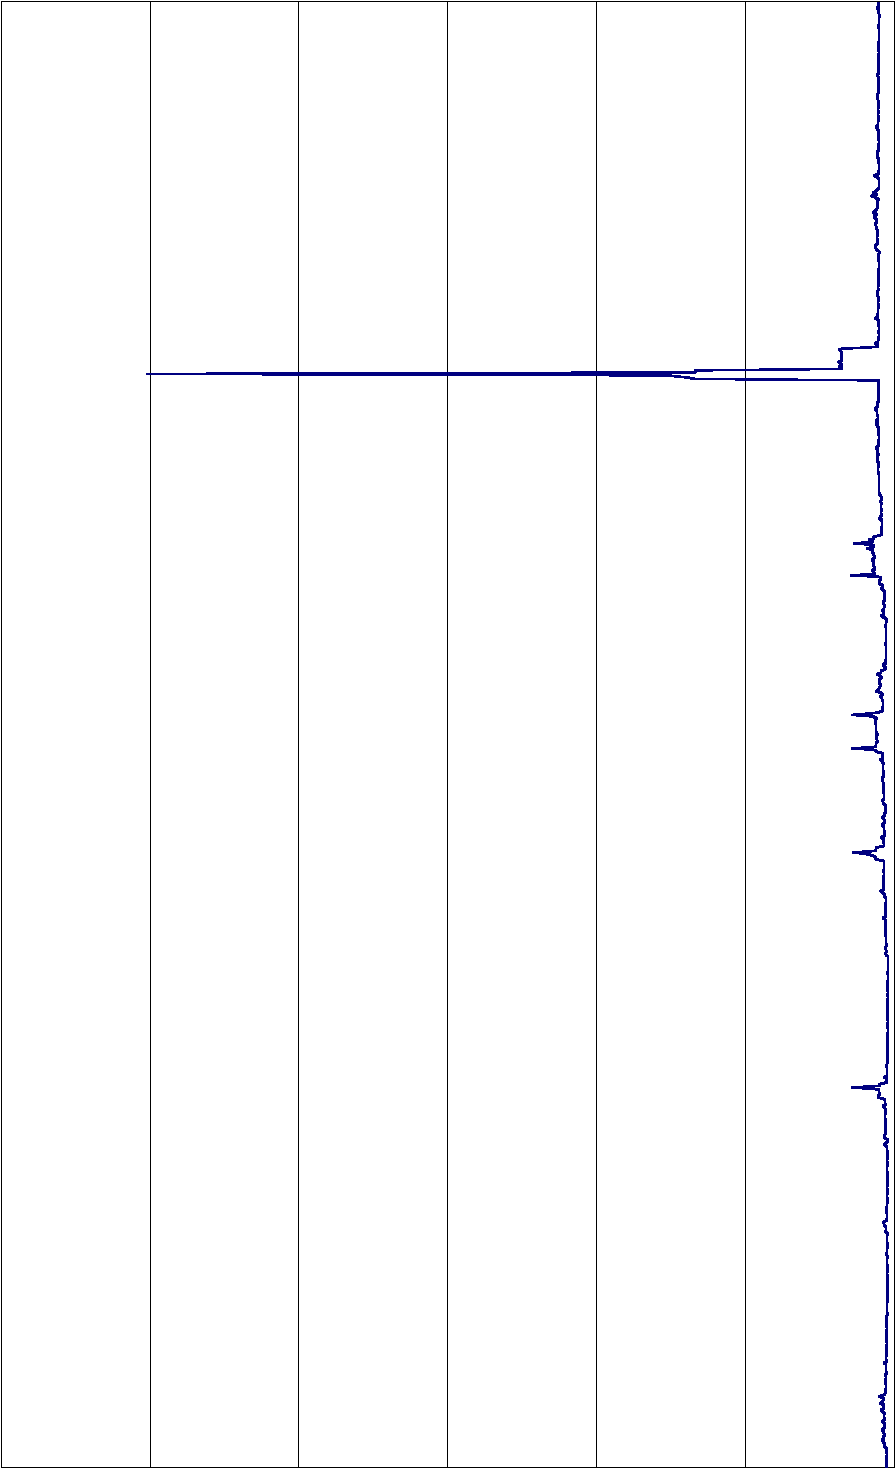
\includegraphics[height=8cm]{2_Etat-art/img/c4paix} }
  \rotatebox{-90}{ 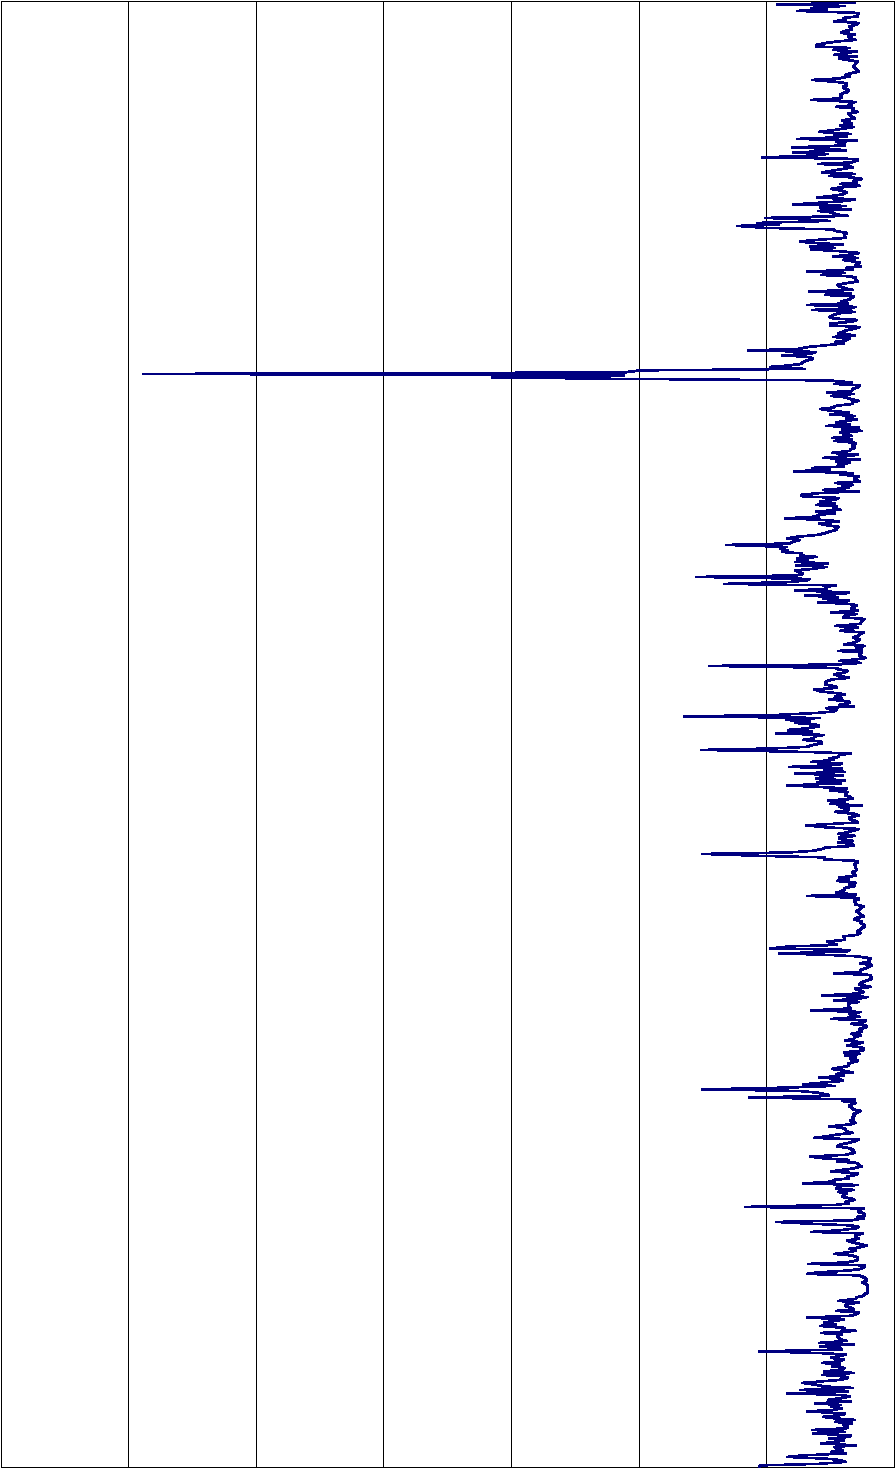
\includegraphics[height=8cm]{2_Etat-art/img/paix} }
    \caption{Vecteurs transversalement augmenté du concept  
      \cname{paix} et pour l'item \lexItem{paix}}
    \label{l2-peace-vector}
\end{figure}

\subsection{Pourquoi nos vecteurs sont-ils dits "conceptuels"?}
\label{sec:pq-nom-VC}

On pourrait penser que le terme \lexItem{conceptuel} qui qualifie nos
vecteurs provient du fait que leur construction est basée sur ces
objets que nous appelons concepts. En pratique, ce nom a été introduit
pour marquer le fait que ces vecteurs représentent des idées plus ou
moins abstraites, plus ou moins générales.

\subsection{Architecture et construction de la base}

Nous présentons succinctement ici l'architecture de la base lexicale
sémantique. %telle qu'elle est conçue au début de nos travaux. Un
%certain nombre de nos choix seront débattus plus avant lorsqu'il sera
%temps, au vue des expériences que nous présentons dans cette partie de
%la thèse, de mettre en place une architecture de base lexicale
%sémantique plus pertinente (cf. chapitre
%\ref{cha:constr-base-lex-sem}). 
Cette architecture est centrée sur le
stockage et l'exploitation de deux objets lexicaux l'objet
\lexobj{item lexical} et l'objet \lexobj{lexie}.

\subsubsection{Structure des objets lexicaux}

Les objets lexicaux sont composés d'un certain nombre
d'\emph{informations linguistiques}~:

\begin{itemize}
\item un \textbf{identifiant};
\item la \textbf{morphologie} composé des \emph{catégories
    grammaticales} (\emph{nom, pronom, adjectif, adverbe, etc.}), du
  \emph{genre} (\emph{masculin, féminin, neutre}) et du nombre
  (\emph{singulier, pluriel});
\item la \textbf{fréquence en usage} c'est-à-dire le nombre de fois
  (ou au moins une estimation) où l'objet a été rencontré;
\item un \textbf{vecteur conceptuel}.
\end{itemize}

\subsubsection{Objets lexicaux} \label{sec:objets-lexicaux}

L'architecture est composée de deux sortes d'objets lexicaux, les
\lexobj{items lexicaux} et les \lexobj{lexies}. Cette architecture
provient essentiellement du mode de fabrication des vecteurs
conceptuels\index{vecteurs! conceptuels} c'est-à-dire à partir de
dictionnaires à usage humain.  \vspace{-0.2cm}
\paragraph{Lexies} \label{sec:lexies}

Les \lexobj{lexies} constituent le socle de la base lexicale
sémantique. À partir de définitions de dictionnaires à usage humain,
il est possible d'extraire un certain nombre d'informations
linguistiques et de calculer un vecteur conceptuel. Examinons, par
exemple, les entrées de \cite{Larousse2004} pour l'item
\lexItem{botte}.
\\
\\
\textbf{1.botte}~: \#nf\# (néerl. bote, touffe de lin) Assemblage de
végétaux de même nature liés ensemble~: (Botte de paille. Botte
de radis.).\\
\textbf{2.botte}~: \#nf\# (\#ethym-it\# botta, coup) . Coup de pointe
donné avec le fleuret ou l'épée.\\
\textbf{3.botte}~: \#nf\# (p.-ê. de bot) . Chaussure à tige montante
qui enferme le pied et la jambe généralement jusqu'au genou~: (Bottes
de cuir).\\

L'idée est pour chacune de ces définitions de fabriquer un objet
\lexobj{lexie} qui comportera~:

\begin{itemize}
\item un \textbf{identifiant}~: habituellement pour les lexies, il est
  constitué du nom du terme et d'un numéro (ex~: \emph{botte.1},
  \emph{botte.2}, \emph{chat.1}, \ldots);
\item la \textbf{morphologie} généralement facile à récupérer
  puisqu'elle est souvent assez bien délimitée;
\item la \textbf{fréquence en usage} qui est estimée par des
  heuristiques, que nous ne détaillerons pas ici, à partir de la
  fréquence de l'\lexobj{item lexical};
\item un \textbf{vecteur conceptuel} calculé à partir du texte de la
  définition grâce à une analyse sémantique telle que celle présentée
  en \ref{sec:an-sem-VC}.
\end{itemize}
  
\paragraph{Items Lexicaux}\label{sec:items-lexicaux}

Les objets \lexobj{items lexicaux} correspondant à un terme sont
fabriqués à partir des \lexobj{lexies} de ce terme. Leur structure est
la suivante~:

\begin{itemize}
\item un \textbf{identifiant} qui est généralement le nom du terme
  (ex~: \emph{botte}, \emph{chat});
\item la \textbf{morphologie} qui rassemble l'ensemble des
  morphologies des lexies;
\item la \textbf{fréquence en usage} qui correspond au nombre de fois
  où le terme a été repéré dans les textes étudiés par l'analyse
  sémantique;
\item un \textbf{vecteur conceptuel} qui est la somme vectorielle
  normée des vecteurs conceptuels\index{vecteurs! conceptuels} des
  lexies.
\end{itemize}

\subsection{Apprentissage des objets lexicaux}
\label{sec:appr-vecteurs}

%Comme nous l'avons vu à propos des vecteurs sémantiques,
%\index{vecteurs! sémantiques}le problème de la couverture lexicale
%s'avère important dès qu'il s'agit d'analyser des textes.  La solution
%choisie pour pallier ce problème a été, pour les vecteurs
%sémantiques,\index{vecteurs! sémantiques} de rajouter une
%représentation vectorielle de type saltonien (cf. méthode mixte
%section \ref{sec:vect-sem-mixte}). Pour les vecteurs
%conceptuels,\index{vecteurs! conceptuels} le choix s'est porté sur un
%apprentissage automatique. Ainsi, l
La fabrication des objets lexicaux
se fait à partir de définitions extraites de dictionnaires à usage
humain sous forme électronique. On crée ainsi une \lexobj{lexie} par
définition puis les objets \lexobj{item lexicaux} à partir de ces
\lexobj{lexies}.

%On voit ici une autre des différences avec les vecteurs sémantiques.
%\index{vecteurs! sémantiques} Alors que ces derniers sont construits
%une fois pour toutes et peuvent donc être utilisés tout de suite dans
%le cadre d'une application, l'apprentissage ne le permet pas dans le
%cas des \index{vecteurs! conceptuels} vecteurs conceptuels.  Nous
%reviendrons plus en détail au chapitre \ref{cha:constr-base-lex-sem}
%sur les raisons qui nous ont poussés à faire ce choix.

\subsubsection{Lexies~: apprentissage à partir de définitions issues de
  dictionnaires classiques}

L'apprentissage à partir de définitions n'est pas sans poser un
certain nombre de problèmes. Il s'agit d'extraire d'un dictionnaire la
ou les entrées correspondant à un terme. À cause de la polysémie ainsi
que de l'homonymie, nous pouvons avoir plusieurs définitions pour une
même entrée. Nous avons divisé en trois étapes successives le
traitement d'une entrée d'un dictionnaire comme nous le présentons sur
la figure \ref{fig:seq-trait-source}~: (1) un \emph{prétraitement}
dont l'objectif est de préparer les données avant les 2 étapes
suivantes.  Il consiste à séparer les différentes définitions et à les
unifier dans un même format prédéfini puis à préparer la définition en
vue d'une analyse sémantique. (2) Une \emph{extraction des
  informations lexicales} et en particulier de la morphologie et enfin
(3) le \emph{calcul d'un vecteur conceptuel} à partir de la définition
formatée.

\begin{figure}[h]
  \centering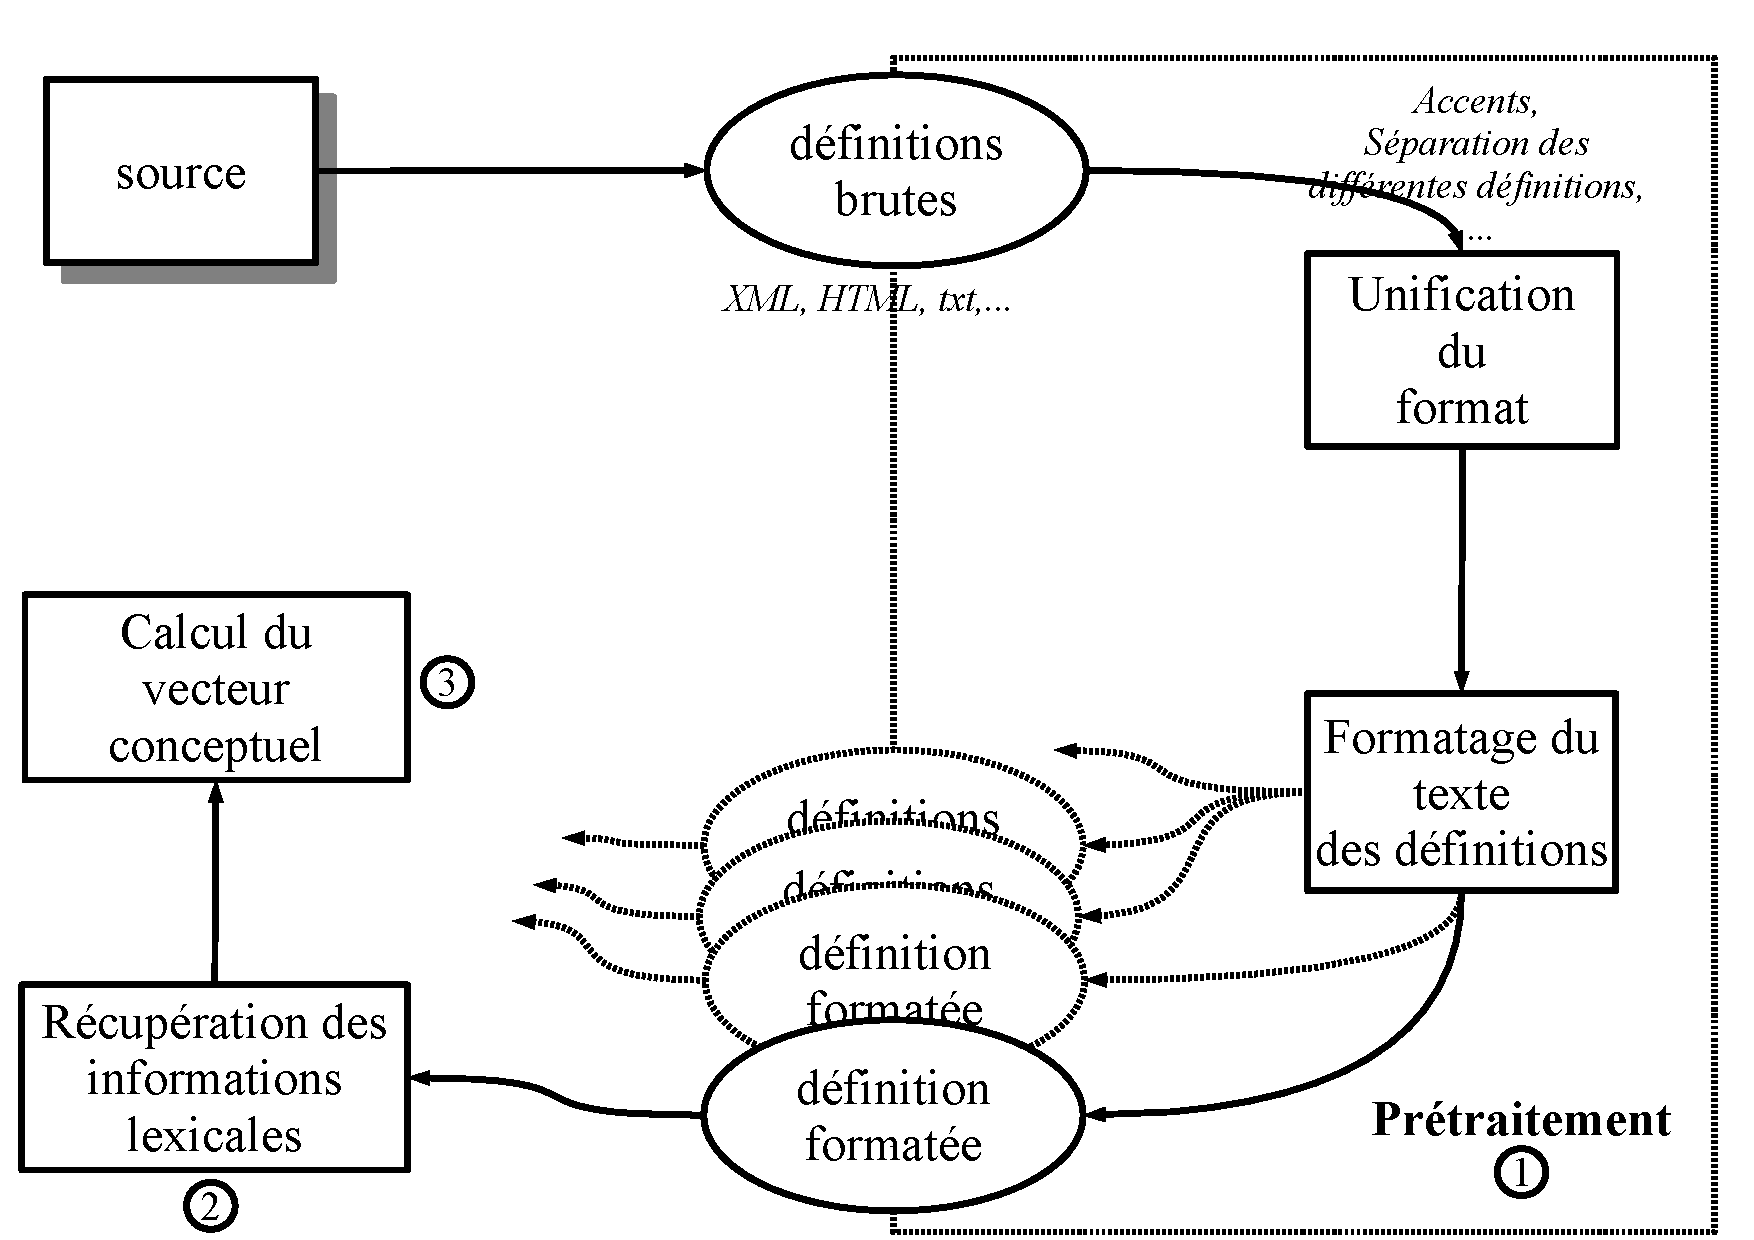
\includegraphics[width=16cm]{2_Etat-art/img/sequences_trait_source}
\caption{Séquence d'opérations pour l'apprentissage de vecteurs
  conceptuels à partir d'une source}
\label{fig:seq-trait-source}
\end{figure}

\paragraph{Prétraitement des données}

La première étape consiste à prétraiter les données. En effet, les
définitions sont extraites de dictionnaires hétérogènes dont le
formatage et les informations disponibles peuvent fortement différer à
la fois pour des raisons purement techniques (codage utilisé, format
des données~: XML, HTML, \ldots) ainsi que pour des raisons formelles
(séparation des sens, des homonymes, \ldots).

Cette opération d'unification du formatage est fondamentale car elle
consiste à convertir le format des données vers un format conçu pour
faciliter l'extraction des informations lexicales ainsi que le calcul
du vecteur conceptuel des définitions. Cette partie de l'apprentissage
est totalement \emph{ad hoc}. Elle doit être conçue pour chaque
dictionnaire afin que les deuxième et troisième étapes soient les
mêmes, quelle que soit la source. Le prétraitement des données
effectue deux catégories de tâches~: une \emph{unification du format}
et un \emph{formatage du texte des définitions}. On appelle
\emph{définitions non formatées} les textes bruts récupérés depuis les
sources et \emph{définitions formatées} les textes obtenus après ce
prétraitement.

\subparagraph{Unification du format}

Les dictionnaires utilisés sont sous forme électronique. Les formats
des données sont très hétérogènes. Nous pouvons avoir de simples
textes comme ceux des dictionnaires papiers, du format HTML pour les
dictionnaires disponibles en ligne ou bien du XML. Il est clair que
suivant le format, il est plus ou moins simple de repérer les
informations pertinentes~: pour le XML, langage balisé généralement de
façon assez claire, beaucoup plus simplement que pour le simple texte
dont il faut chercher à repérer de façon souvent beaucoup plus
heuristique les schémas permettant de détecter la morphologie et les
séparations entre les différentes définitions. En revanche, un certain
nombre de caractères spéciaux (lettres avec diacritiques,
symboles,~\ldots) devront être convertis dans le cas du HTML.

\subparagraph{Formatage du texte des définitions}
\label{sec:formatage-defs}

Cette opération vise à préparer l'apprentissage des vecteurs
conceptuels\index{vecteurs! conceptuels} grâce aux textes des
définitions. Le formatage est employé à plusieurs niveaux~:

\begin{itemize}
    
\item \emph{Gestion du métalangage} L'apprentissage va s'effectuer
  grâce à une méthode d'analyse sémantique telle que celle présentée
  en \ref{sec:remonte-redescente}. Comme nous l'avons vu, il est
  parfois nécessaire de préformater les textes afin de simplifier
  l'apprentissage. L'étude des définitions pose en particulier des
  problèmes essentiellement à cause du \emph{métalangage},
  c'est-à-dire le langage utilisé pour structurer le discours.  Un
  certain nombre de tournures caractérisent ce métalangage et ne sont
  pas porteuses de sens~: \lexItem{se dit de}, \lexItem{relatif à},
  \lexItem{action de}, \lexItem{nom usuel de}, \lexItem{Abr. de},
  \ldots
  
  Ce prétraitement consiste à rechercher ces tournures dans les
  définitions et à les remplacer par un symbole.  L'analyseur
  sémantique lorsqu'il le rencontre ne lui attribue aucune sémantique.
  Ainsi, ces symboles ne seront absolument pas utilisés dans le calcul
  des vecteurs car considérés comme non porteurs de sens par
  l'analyseur sémantique.  Nous avons répertorié à ce
  jour\footnote{Mars 2005} un peu moins de 80 tournures. Ce chiffre
  est en constante augmentation au fur et à mesure de la découverte de
  nouveaux cas, phénomène de plus en plus rares toutefois.
  
\item \emph{balisage de la morphologie} Cette opération est assez
  simple, la morphologie étant généralement bien indiquée.
  
\item \emph{formatage des informations thématiques} Ce prétraitement
  exploite aussi des informations qui peuvent permettre par la suite
  d'aider l'analyse sémantique. C'est le cas en particulier du domaine
  qui est un très bon indice du \index{champ sémantique} champ
  sémantique des items constituant une définition. En pratique ceux-ci
  sont remplacés par des concepts (par exemple, le domaine
  \emph{COMM.} sera remplacé par \cname{commerce} et \emph{BOURSE} par
  \cname{bourse}). De même, certains dictionnaires fournissent des
  résumés d'où on peut extraire certaines informations simples. Par
  exemple, un résumé indiquant \emph{poète français} sera annoté par
  le concept \cname{poésie} tandis qu'un résumé indiquant
  \emph{dramaturge} sera annoté par \cname{théâtre}.

\end{itemize}

\paragraph{Extraction des informations lexicales}

La deuxième étape de l'apprentissage de lexies consiste à extraire les
informations lexicales. Pour l'instant, cette partie de
l'apprentissage ne consiste qu'en l'extraction des informations
concernant la morphologie. Nous verrons dans les chapitres suivants
l'ajout d'autres informations lexicales en particulier des
informations concernant les relations lexicales.

\paragraph{Calcul des vecteurs conceptuels}\index{vecteurs! conceptuels}

L'analyse des définitions se fait grâce à la méthode d'analyse
sémantique présentée en \ref{sec:an-sem-VC}. Les définitions formatées
au cours du pré-traitement sont analysées et le vecteur résultant de
l'analyse est affecté à la lexie.

\subsubsection{Noyau} \label{sec:noyau}\index{vecteurs! conceptuels}

Afin d'amorcer le système d'apprentissage, une partie des termes est
indexée de façon manuelle. Ce noyau est constitué d'un ensemble de
termes choisis parmi les plus courants et/ou les plus polysémiques.
Il s'agit donc de fabriquer manuellement les \lexobj{lexies} de ces
items lexicaux particuliers. L'identifiant et la morphologie sont
remplis de manière triviale, la fréquence est, comme pour tous les
objets lexicaux, nulle à la création. Le vecteur conceptuel associé à
la lexie est fabriqué par la somme pondérée des vecteurs génératifs
\index{vecteurs génératifs} correspondant aux concepts présents dans
cette lexie. Par exemple, nous avons pour l'item lexical
\lexItem{paix} les lexies manuellement indexées suivantes~:

\begin{quotation}\noindent
  \begin{itemize}
  \item \textbf{identifiant}~: paix.1
  \item \textbf{morphologie}~: \morpho{[nom]}
  \item \textbf{fréquence en usage}~: 0
  \item \textbf{vecteur conceptuel}~: $V($\cname{paix}$) \vecadd
    \frac{1}{2} V($\cname{guerre}$) \vecadd V($\cname{sécurité}$)
    \vecadd \frac{1}{2} V($\cname{accord}$)$
  \end{itemize}
  
  \vspace{0.5cm}
  
  \begin{itemize}
  \item \textbf{identifiant}~: paix.2
  \item \textbf{morphologie}~: \morpho{[nom]}
  \item \textbf{fréquence en usage}~: 0
  \item \textbf{vecteur conceptuel}~: $V($\cname{repos}$) \vecadd
    V($\cname{calme}$) \vecadd V($\cname{silence}$) \vecadd
    \frac{1}{2} V($\cname{équilibre}$)$
  \end{itemize}
\end{quotation}

Deux sens ont été indexés pour \lexItem{paix}.  Le premier se réfère à
une \textit{absence de guerre} et le deuxième à une \textit{situation
  de calme}. L'énumération des concepts pondérés est une tâche
difficile car subjective. Dans notre expérimentation, nous laissons
cette tâche aux lexicographes qui ont créé le thésaurus Larousse
\cite{Thesaurus1992} (cf. \ref{sec:thes-larousse}) pour les concepts
ainsi que les dictionnaires \cite{Larousse2001} et \cite{Robert2000}
pour les découpages de sens. Seuls les mots parmi les plus importants
sont ainsi décrits dans le noyau. Nous nous reposons sur
l'apprentissage automatique pour l'indexation en masse. Toutefois, les
séparations délicates de sens nécessitent des ajustements manuels.

Les items lexicaux de ce noyau sont considérés comme pertinents.  Cet
ensemble constitue la base d'items lexicaux à partir de laquelle
démarre l'apprentissage (cf. figure \ref{fig:noyau}).  Nous cherchons
à mettre au point un apprentissage qui soit le plus cohérent possible
afin d'obtenir une base augmentée pertinente. Dans ce chapitre, cet
apprentissage se fait uniquement à partir de dictionnaires mais, dans
les suivants, il sera basé, en partie, sur les relations sémantiques,
en particulier symétriques, comme la synonymie et l'antonymie.

\begin{figure}[h]
  \centering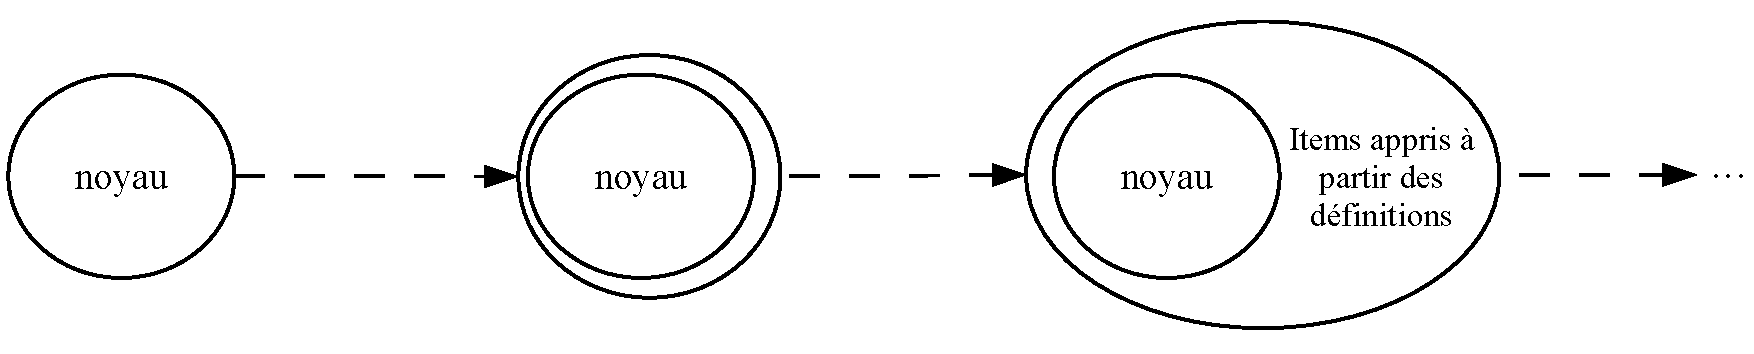
\includegraphics[width=16cm]{2_Etat-art/img/augmentation-noyau}
\caption{Augmentation de la couverture lexicale grâce à l'apprentissage}\label{fig:noyau}
\end{figure}

\subsection{Contextualisation forte}\index{vecteurs! conceptuels}
\label{sec:context-forte}

\subsubsection{Définition}

Tandis que la méthode de contextualisation faible peut être utilisée
avec n'importe quel vecteur (cf. \ref{sec:cont-faible}), la méthode de
contextualisation forte est utilisée, elle, avec les \lexobj{items
  lexicaux}. L'idée est de considérer les vecteurs
conceptuels\index{vecteurs! conceptuels} associés à chacune des
\lexobj{lexies} de l'item en fonction des informations contextuelles
disponibles.  Ces informations peuvent être alors non seulement
d'ordre vectoriel mais aussi d'ordre morphologique. Ainsi, lors d'une
analyse sémantique, les informations morphologiques des feuilles
peuvent être utilisées grâce à cette méthode. La méthode de
contextualisation forte ne fait donc pas un choix parmi les divers
vecteurs des \lexobj{lexies}, mais en favorise certains aux détriments
d'autres. La fonction de contextualisation forte est ainsi définie
par~:

\begin{center}

  \begin{tabular}{ccc}
    $\EnsIL\times \EnsMorpho \times\EnsVC \rightarrow \EnsVC$&:&$V =
    \strongcon(I, M_{c}, V_{c})$\\    
  \end{tabular}
\end{center}

où $\EnsIL$ est l'ensemble des \lexobj{items lexicaux}, $\EnsMorpho$
l'ensemble des morphologies et $\EnsVC$ l'ensemble des vecteurs
conceptuels.\index{vecteurs! conceptuels}

Il s'agit ici d'un principe général et diverses méthodes ont été
testées. Celle qui suit est actuellement utilisée dans le cadre du projet VidéoSense
%l'expérimentation effectuée sur les vecteurs
%conceptuels\index{vecteurs! conceptuels} au cours de ma thèse dont
%l'implémentation est présentée en \ref{sec:constr-et-expl}. D'autres
%expérimentations ont été menées par \index{Lafourcade Mathieu} Mathieu
%Lafourcade sur sa propre base de vecteurs conceptuels.

\index{vecteurs! conceptuels}
  
\begin{equation}
  \begin{array}{c}
  \strongcon(I, M_{c}, V_{c}) = \bigvecadd_{L_i}
  (P_i\vecptt V(L_i))\\\\
  \mbox{ où } P_i = P_{morpho}(L_i, M_c)^l \times P_{ang}(L_i,
    V_c)^m \times P_{\mbox{\emph{freq}}}(L_i)^n\\\\
    \mbox{et } l, m, n \in \{0,1\}
  \end{array}
\end{equation}

où $I$ représente l'item dont on cherche le vecteur contextualisé et
qui est composé d'un ensemble de \lexobj{lexies} \{$L_1$, $L_2$,
\dots, $L_i$, \ldots, $L_n$\}, $P_{morpho}$ le poids morphologique,
$P_{ang}$ le poids angulaire et $P_{\mbox{\emph{freq}}}$ le poids de
la fréquence, tous trois définis ci-après.

Le poids $P_i$ est donc la moyenne géométrique pondérée des poids
morphologique, angulaire et de fréquence des lexies. Suivant les
utilisations de la méthode de contextualisation forte, l'une ou
l'autre des informations contextuelles peut ainsi être favorisée ou au
contraire être ignorée. Ainsi, dans le cas de l'apprentissage, les
exposants $l, m, n$ valent $1$, tandis que dans le calcul du vecteur
d'un \lexobj{item lexical}, aucun des critères n'est considé
($l=m=n=0$), ce qui correspond à la somme vectorielle normée des
vecteurs des \lexobj{lexies} (cf.  \ref{sec:items-lexicaux}).
  
%Sauf indication contraire, nous utiliserons, dans la suite de cette
%thèse, une méthode de contextualisation forte où $l = m = n = 1$.

\subsubsection{Poids angulaire}\index{vecteurs! conceptuels}

\begin{equation}
\EnsLex \times \EnsVC \rightarrow [0, k]~: P_{ang}(L,X) =
Min(k,cotan(\mbox{\dang{V(L)}{X}}))
\end{equation}

où $cotan$ est la fonction cotangente, l'inverse de la fonction
tangente ($\frac{1}{tan(x)}$). Expérimentalement, nous avons posé
$k=10$.

\subsubsection{Poids de la fréquence}\index{vecteurs! conceptuels}

\begin{equation}
\EnsLex \rightarrow [0,1]~: P_{\mbox{\emph{freq}}} = \frac{\freq{L}}{\freq{item(L)}}
\end{equation}

où $item(L)$ renvoi l'\lexobj{item lexical} correspondant à la
\lexobj{lexie} L et $\freq{x}$ renvoie la fréquence de l'objet lexical
$x$.

  \subsubsection{Poids et distance morphologique}\label{sec:poids-et-distance-morpho}\index{vecteurs! conceptuels}
  
  Soit le poids morphologique $P_{morpho}$ défini par~:

  \begin{equation}
  \EnsMorpho\times\EnsMorpho \rightarrow [0, \frac{\pi}{2}]~: P_{morpho}
  (M_1, M_2) = \frac{\pi}{2} - arctan(D_{morpho}(M_1,M_2))
  \end{equation}
  
  $M_1$ et $M_2$ sont des ensembles au sens mathématique du terme. Par
  exemple, la morphologie de \lexItem{botte} peut être vue comme
  l'ensemble à deux éléments \{\emph{nom}, \emph{masculin}\} et celle
  de \lexItem{orgues} comme l'ensemble à trois éléments \{\emph{nom},
  \emph{masculin}, \emph{pluriel}\}.
  
  Par définition, on pose~:

\begin{equation}
P_{morpho}(M_1,M_2) =
\frac{\pi}{2} \mbox{ si } M_1 = \varnothing \mbox{ ou }M_2 =
\varnothing.\label{eq:4}
\end{equation}
  
La mesure du poids est calculée comme suit~:

\begin{equation}
  D_{morpho}(M_1,M_2) = \sum_{x\in (M_1 \cup M_2) - (M_1\cap M_2)} p(X) \mbox{ où } \left\{
  \begin{array}{l}
    p(X) = 1 \mbox{ si } X \mbox{ est une catégorie grammaticale}\\
    p(X) = 0,5 \mbox{ sinon}
  \end{array}
  \right.
\end{equation}

Cette distance est donc uniquement fonction de ce qui sépare les deux
morphologies. Par exemple, la distance morphologique entre
\{\emph{nom}, \emph{masculin}\} et \{\emph{nom}, \emph{masculin},
\emph{plur}\} ne sera que fonction de \emph{plur} et vaudra ainsi
$0,5$. De fait, nous avons $D_{morpho}(X,X)=0$. Voici quelques
exemples de poids et de distances morphologiques~:

\begin{center}
  \begin{tabular}{cccc}
    $morpho_1$&$morpho_2$&$D_{morpho}$&$P_{morpho}$\\
    \{nom\} & \{nom\} & 0& $\frac{\pi}{2}$\\%0\\
    \{nom, masc\} & \{nom, masc\} & 0& $\frac{\pi}{2}$\\%0\\
    \{nom, masc\} & \{nom\} & 0,5& 1,11\\%0,46\\
    \{nom, masc\} & \{fem\} & 2& 0,47\\%\\1.1\\
    \{nom, masc\} & \{nom, fem\} & 1& 0,79\\%0,78\\
    \{verbe\} & \{nom\} & 1,25& 0,68\\%0,89\\
    \{verbe, intransitif\} & \{nom masc plur\} & 2,75& 0,35\\%1,22\\

\end{tabular}
\end{center}

\subsection{Analyse sémantique des textes en remontée-redescente grâce aux vecteurs
  conceptuels}\index{vecteurs! conceptuels}
\label{sec:an-sem-VC}

\index{analyse sémantique! par remontée-redescente!
(vecteurs conceptuels)}

\subsubsection{Algorithmes}

L'analyse sémantique des textes en remontée-redescente à l'aide des
vecteurs conceptuels\index{vecteurs! conceptuels} est permise par les
algorithmes \ref{algo:AS-VC1} et \ref{algo:AS-VC2}.

\begin{algorithm}[h]
  \Entree{vecteur conceptuel $V_{contexte}$, $A$ arbre
    morpho-syntaxique du texte, seuil $s$} \Sortie{vecteur conceptuel
    du texte}
  
  Vecteur $V$ = analyse ($V_{contexte}$, A.racine)
  
  \Repeter{(\dang{$V$}{$V_2$}<$s$)}{
    Vecteur $V_2$ = $V$\\
    $V$ = analyse($V$, A.racine)} \Retour $V$
\caption{analyse~: algorithme d'analyse sémantique avec les vecteurs conceptuels}
  \label{algo:AS-VC1}
\end{algorithm}
  
\begin{algorithm}[h]
  \Entree{vecteur conceptuel $V_{contexte}$, n\oe ud N}
  \Sortie{vecteur conceptuel du sous-arbre de N} \Si{N est une
    feuille}{ \Si{N.item.estUnMotVide()}{ N.vecteur=$V_{\veczero}$}
    \Sinon{N.vecteur=$\strongcon$(N.item, N.morpho, $V_{contexte}$)}
    \Si{N.estGouverneur}{ N.vecteur = $2\vecptt$N.vecteur }
    \Retour{N.vecteur} } \Sinon{
    $V = \veczero$\\
    \Pour{chacun des fils $f_i$ de N}{
      $V = V + analyse(\con(N.vecteur,V_{contexte}), f_i)$\\
      N.vecteur=norm(V) } }
\caption{algorithme d'analyse sémantique avec les vecteurs conceptuels
  : analyse}
  \label{algo:AS-VC2}
\end{algorithm}


\subsubsection{Principe}
Le principe est de faire descendre les informations du vecteur
contexte du texte jusqu'aux feuilles de l'arbre en les enrichissant
par les informations contenues dans les n\oe uds de l'arbre.  Dans le
cas général où nous n'avons aucune information thématique au début de
l'analyse, le vecteur contexte utilisé lors de la première descente
est le vecteur nul. Dans d'autres cas, l'analyse de définitions par
exemple, si des informations du domaine sont spécifiées, le vecteur
contexte utilisé sera celui de ce domaine.

Dans un arbre morpho-syntaxique, les feuilles contiennent les
informations sur les items ainsi que leur morphologie dans le texte.
Ces deux informations sont utilisées pour calculer les vecteurs
correspondant aux contextualisations fortes de ces items
(cf.~\ref{sec:context-forte}) et les affecter à chacune des feuilles
de l'arbre. Les feuilles qui correspondent à des mots vides de sens
(déterminants, conjonction de coordination, préposition, \ldots) se
voient affecter un vecteur vide.

La remontée se fait alors de la même manière que celle de l'analyse
avec les \index{vecteurs! sémantiques} vecteurs sémantiques. Les
vecteurs de chaque n\oe ud sont calculés à partir des vecteurs de
leurs fils et de pondérations calculées en fonction de leur rôle
syntaxique. Le vecteur de chaque n\oe ud est ainsi calculé
récursivement jusqu'au sommet de l'arbre. Ce vecteur possède les idées
contenues dans tout mot du texte. À ce moment du calcul, il n'y a eu,
dans le cas général, aucune contextualisation. Le vecteur du sommet de
l'arbre contient donc les idées pertinentes du texte mais aussi
beaucoup de bruit. On effectue à nouveau une descente. On calcule la
contextualisation faible du vecteur de chacun des n\oe uds en fonction
de celui de son père.  Ainsi, le vecteur contexte n'est pas le même
pour tous les n\oe uds de l'arbre mais est plus directement fonction
du sous-arbre dont il est ancêtre. Cette solution améliore largement
l'analyse dans le cas d'une phrase comme \sentence{La souris
  d'ordinateur est posée sur la table du vétérinaire.}. En effet, si
on n'utilise pas un tel mécanisme, le sens de souris serait autant
influencé par l'idée d'\cname{informatique} contenue dans
\lexItem{ordinateur} que par celle d'\cname{animal} contenue dans
\mot{vétérinaire}, ce qui empêcherait la désambiguïsation du texte.

Au niveau des feuilles, on effectue une contextualisation forte puis
une remontée. Ces opérations sont renouvelées un certain nombre de
fois jusqu'à une relative stabilisation du vecteur général
c'est-à-dire tant que la distance angulaire entre deux vecteurs du
sommet calculés successivement n'est pas inférieure à un certain seuil
$s$.

\subsubsection{Exemple}

La figure
\ref{fig:an-sem-VC} présente l'analyse sémantique de \sentence{La souris d'ordinateur.} grâce aux
\index{vecteurs! conceptuels} vecteurs conceptuels. Considérons le cas
général où le vecteur contexte est nul. Nous le faisons redescendre
jusqu'aux feuilles de l'arbre en faisant une contextualisation faible
aux vecteurs de chaque n\oe ud.  Bien entendu, lors de cette première
descente, tous ces vecteurs seront nuls. Les feuilles $2$ et $5$ qui
correspondent respectivement à un déterminant et à une préposition et
qui sont donc des mots vides de sens se voient affectées d'un vecteur
nul. En revanche, le n\oe ud $3$ se voit affecté du vecteur conceptuel
correspondant à la contextualisation forte de \lexItem{souris} avec la
morphologie \emph{nom fem} et le vecteur contexte nul. La même
opération est réalisée sur le noeud $5$ avec \lexItem{ordinateur} et
\emph{nom masc}.

Lors de la remontée, le n\oe ud $4$ est affecté par le vecteur
correspondant à la somme vectorielle pondérée entre ses deux n\oe uds
fils $5$ et $6$. Le vecteur de la feuille est considéré avec un poids
de 2 pour cette opération puisqu'il est gouverneur syntaxique du
sous-arbre correspondant à \sentence{d'ordinateur}. Il en est de même
pour le vecteur du n\oe ud $3$ (\lexItem{souris}) dans le calcul du
vecteur global du texte.

L'opération de redescente-remontée se renouvelle ainsi de suite
jusqu'à une stabilisation du vecteur global du texte.

\index{analyse sémantique! par remontée-redescente!
(vecteurs conceptuels)}

\begin{figure}[h]
  
  \centering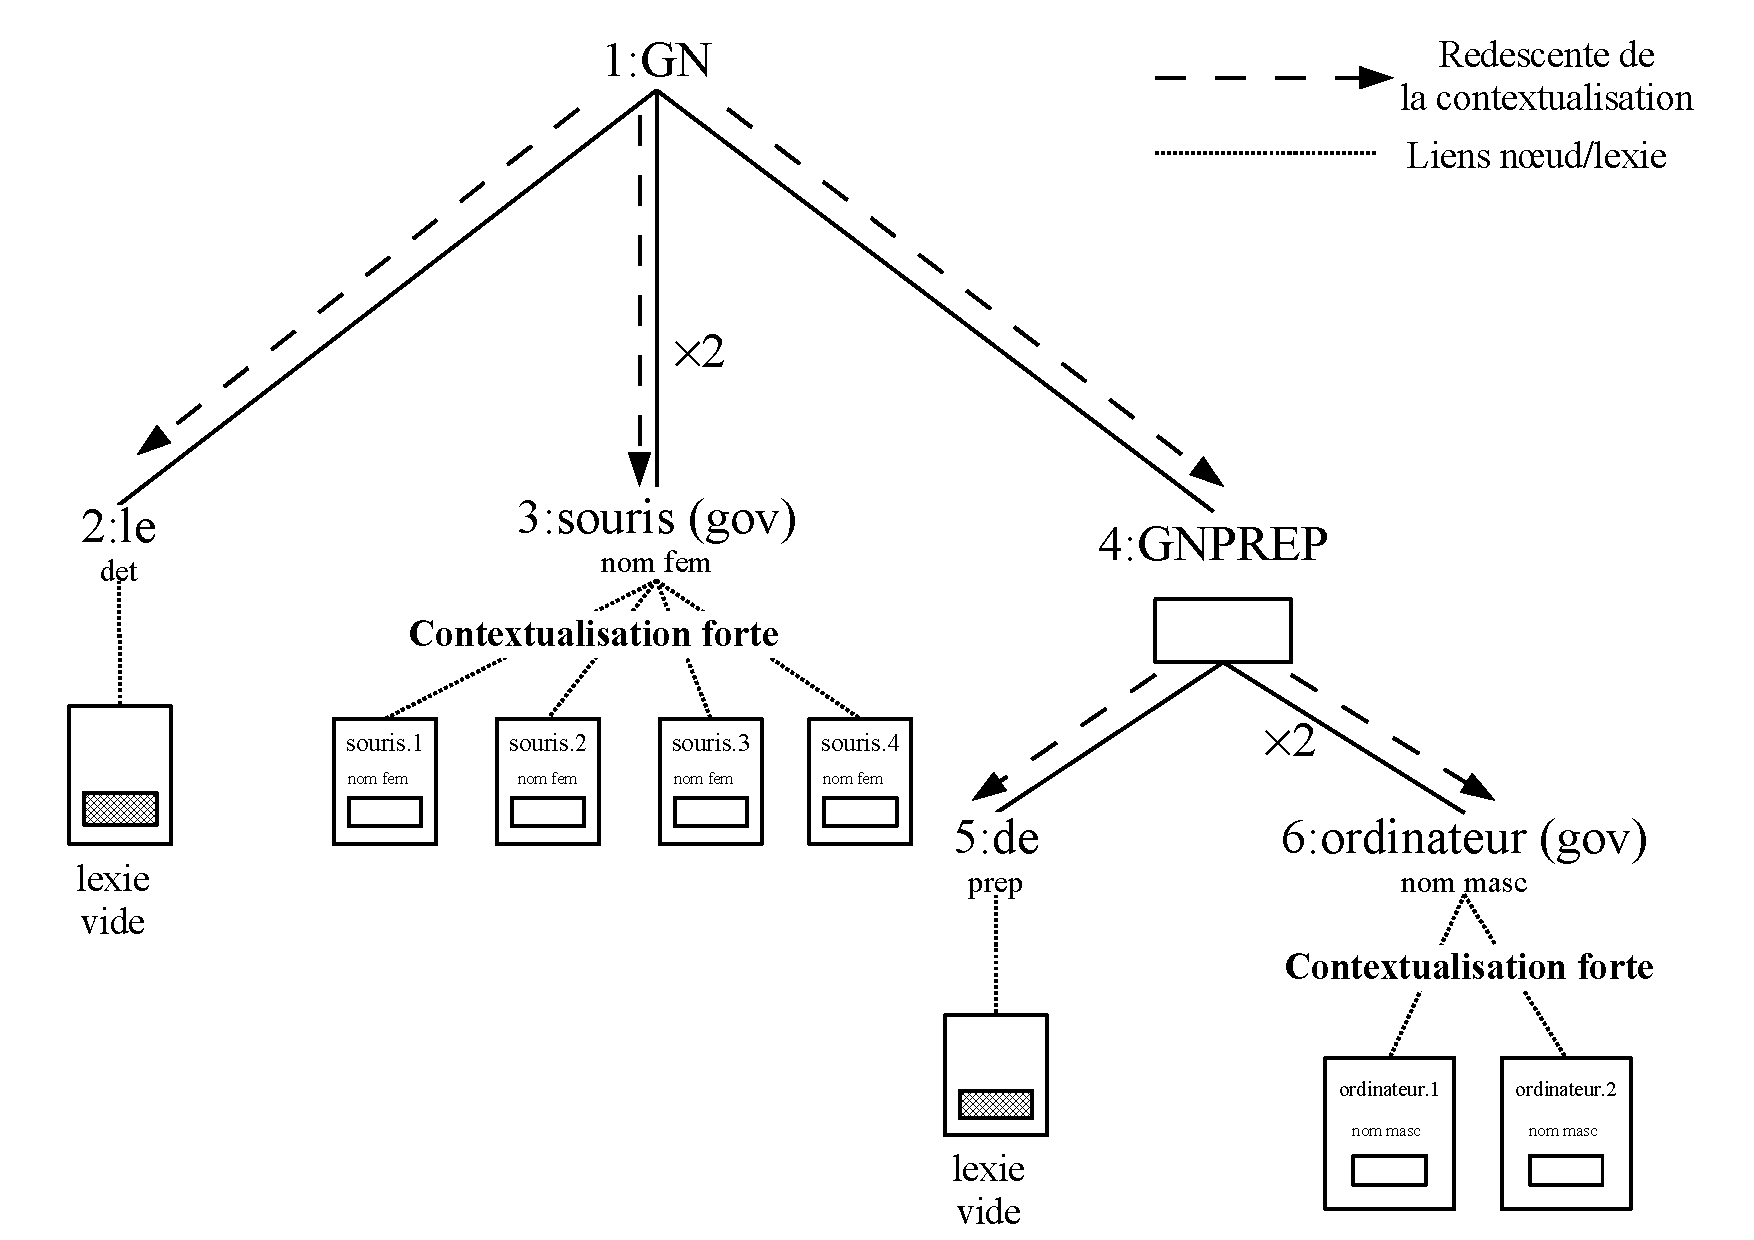
\includegraphics[width=16cm]{2_Etat-art/img/an-sem-VC-souris-de-lordi}
\caption{Exemple d'analyse sémantique grâce aux vecteurs conceptuels}
\label{fig:an-sem-VC}
\end{figure}

\subsection{Construction des vecteurs par émergence}
\label{sec:emergence}

Nous utilisons dans le cadre de VideoSense, une deuxième manière de construire les vecteurs conceptuels : par émergence. Cette approche s'affranchit de tout thésaurus et vecteurs de
concept comme base de départ. Seule $d$ %, la dimension de la base de
%l'espace vectoriel, c'est-à-dire
la taille du vecteur est fixée \emph{a priori}. Le mode de
construction des vecteurs est identique au modèle classique à la
différence que si un des vecteurs entrant dans la somme est
inexistant, car non encore calculé, alors ce vecteur est tiré au
hasard. Le processus de calcul est itéré jusqu'à convergence de chaque
vecteur.

%\#\#\#\#\#\#\#\#\#

%Didier -> Utiliser dimension ne veut-il pas dire que la base est libre
%puisque dimension = taille. Est-ce utile ? ça apporte quelque chose ou
%ça risque de faire tiquer pour rien ?

%Mathieu -> pas faux : j'ai sutilement modifié - ca suffit tu crois ?

%Didier -> dimension de l'espace = dimension de la base, peut être
%éluder la question en ne parlant que de la dimension des vecteurs

%\#\#\#\#\#\#\#\#\#

Comme nous le montre de façon plus détaillée \cite{Lafourcade-emergence2006}, il y a un certain nombre d'avantages à
utiliser ce modèle. Le premier d'entre eux est de pouvoir choisir
librement la quantité de ressources que l'on souhaite utiliser en
choisissant la taille des vecteurs de façon appropriée. Pour donner
une idée de l'importance de ce choix, une base de 500000 vecteurs de
dimension 1000 fait environ 2Go, de taille 2000, 4Go,~\ldots~Comme il
ne serait pas alors ni raisonnable ni facile de définir un jeu de
concept de la taille choisie, autant chercher une approche nous
permettant de nous en passer. De plus, ce qui peut sembler un
pis-aller ou au mieux un compromis, s'avère un avantage car la densité
lexicale dans l'espace des mots calculés par émergence est bien plus
constante que dans un espace où les concepts sont précalculés. En
effet, les ressources (les dimensions de l'espace) ont tendance à être
harmonieusement distribuées en fonction de la richesse lexicale.

